\appendix
\addcontentsline{toc}{section}{Appendici}
%\section*{Appendici}
\newsection{Copertura dei requisiti}
\normalsize
\renewcommand{\arraystretch}{1.5}
\begin{longtable}{|c|c|}
	\hline
	\rowcolor{title_row}
	\textbf{\color{title_text}{Requisito}} & \textbf{\color{title_text}{Stato}} \\
	\hline
	\endhead
	{R0F1} & Implementato\\
	\hline
	{R1F1.1} & Implementato\\
	\hline
	{R0F2} & Implementato\\
	\hline
	{R0F2.1} & Implementato\\
	\hline
	{R0F2.2} & Implementato\\
	\hline
	{R1F2.3} & Implementato\\
	\hline
	{R0F3} & Implementato\\
	\hline
	{R1F3.1} & Implementato\\
	\hline
	{R0F4} & Implementato\\
	\hline
	{R1F4.1} & Implementato\\
	\hline
	{R0F5} & Implementato\\
	\hline
	{R1F5.1} & Implementato\\
	\hline
	{R1F5.2} & Implementato\\
	\hline
	{R1F5.3} & Implementato\\
	\hline
	{R1F5.4} & Implementato\\
	\hline
	{R1F5.5} & Implementato\\
	\hline
	{R1F5.6} & Implementato\\
	\hline
	{R1F5.6.1} & Implementato\\
	\hline
	{R1F5.6.2} & Implementato\\
	\hline
	{R1F5.6.3} & Implementato\\
	\hline
	{R1F5.7} & Implementato\\
	\hline
	{R1F5.7.1} & Implementato\\
	\hline
	{R1F6} & Implementato\\
	\hline
	{R1F6.1} & Implementato\\
	\hline
	{R1F6.1.1} & Implementato\\
	\hline
	{R1F6.1.2} & Implementato\\
	\hline
	{R1F6.1.3} & Implementato\\
	\hline
	{R1F6.2} & Implementato\\
	\hline
	{R1F7} & Non implementato\\
	\hline
	{R1F7.1} & Non implementato\\
	\hline
	{R1F7.1.1} & Non implementato\\
	\hline
	{R1F7.1.2} & Non implementato\\
	\hline
	{R1F7.1.3} & Non implementato\\
	\hline
	{R1F7.1.4} & Non implementato\\
	\hline
	{R1F7.1.4.1} & Non implementato\\
	\hline
	{R1F7.1.4.2} & Non implementato\\
	\hline
	{R1F7.1.4.3} & Non implementato\\
	\hline
	{R1F7.2} & Non implementato\\
	\hline
	{R1F7.2.1} & Non implementato\\
	\hline
	{R1F7.2.2} & Non implementato\\
	\hline
	{R1F7.2.2.1} & Non implementato\\
	\hline
	{R1F7.2.2.2} & Non implementato\\
	\hline
	{R1F7.2.2.3} & Non implementato\\
	\hline
	{R1F7.2.2.3.1} & Non implementato\\
	\hline
	{R1F7.2.2.3.2} & Non implementato\\
	\hline
	{R1F7.2.2.4} & Non implementato\\
	\hline
	{R1F7.3} & Non implementato\\
	\hline
	{R1F7.4} & Non implementato\\
	\hline
	{R1F7.4.1} & Non implementato\\
	\hline
	{R1F7.4.2} & Non implementato\\
	\hline
	{R1F7.5} & Non implementato \\ 
	\hline
	{R1F7.6} & Non implementato\\
	\hline
	{R1F7.6.1} & Non implementato\\
	\hline
	{R1F7.6.2} & Non implementato\\
	\hline
	{R1F7.7} & Non implementato\\
	\hline
	{R1F7.7.1} & Non implementato\\
	\hline
	{R1F7.7.2} & Non implementato\\
	\hline
	{R1F7.7.3} & Non implementato\\
	\hline
	{R1F7.7.4} & Non implementato\\
	\hline
	{R2F8} & Non implementato\\
	\hline
	{R2F9} & Non implementato\\
	\hline
	{R2F10} & Implementato\\
	\hline
	{R2F10.1} & Implementato\\
	\hline
	{R2F10.2} & Implementato\\
	\hline
	{R2F10.3} & Implementato\\  
	\hline
	{R2F10.3.1} & Implementato\\ 
	\hline
	{R2F10.3.2} & Implementato \\ 
	\hline
	{R2F10.3.3} & Implementato \\ 
	\hline
	{R2F10.3.4} & Implementato \\
	\hline                              
	{R2F10.3.5} & Implementato\\
	\hline
	{R2F10.4} & Implementato\\
	\hline
	{R2F10.4.1} & Implementato\\
	\hline
	{R2F10.4.2} & Implementato\\
	\hline
	{R2F10.4.3} & Implementato\\
	\hline
	{R2F10.4.3.1} & Implementato\\
	\hline
	{R2F10.4.3.2} & Implementato\\
	\hline
	{R2F10.4.3.3} & Implementato\\
	\hline
	{R2F10.5} & Implementato\\
	\hline
	{R2F10.6} & Implementato\\
	\hline
	\caption[Copertura requisiti funzionali]{Copertura requisiti funzionali}
	\label{}
\end{longtable}
\renewcommand{\arraystretch}{1}

\newpage
\subsection{Resoconto copertura dei requisiti}
\begin{itemize}
	\item \textbf{Requisiti obbligatori}
	\begin{figure} [H]
		\centering
		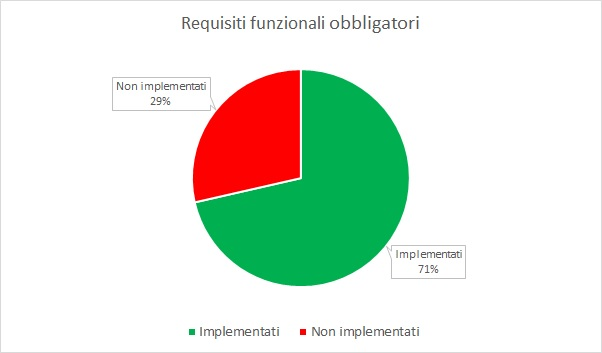
\includegraphics[scale=1]{Img/R0}
		\caption{Resoconto requisiti funzionali obbligatori}
	\end{figure}
	\item \textbf{Requisiti desiderabili}
	\begin{figure} [H]
		\centering
		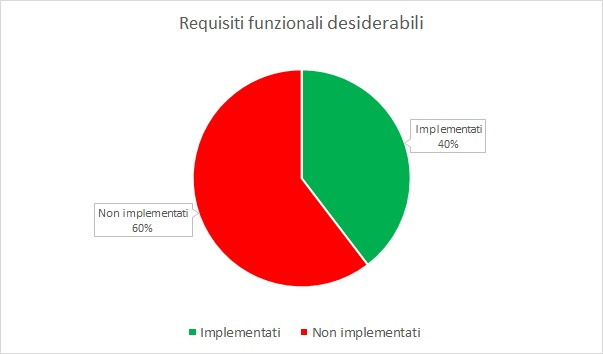
\includegraphics[scale=1]{Img/R1}
		\caption{Resoconto requisiti funzionali desiderabili}
	\end{figure}
\newpage
	\item \textbf{Requisiti opzionali}
	\begin{figure} [H]
		\centering
		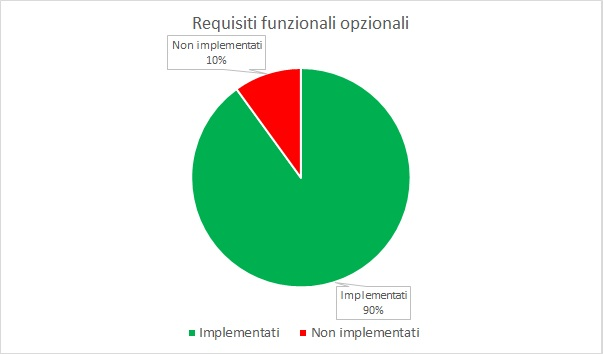
\includegraphics[scale=1]{Img/R2}
		\caption{Resoconto requisiti funzionali opzionali}
	\end{figure}
\end{itemize}

\newpage


\newsection{Resoconto delle attività di verifica}

\subsection{Revisioni}
Questa sezione riporta il resoconto delle attività di verifica svolte prima di ciascuna delle quattro revisioni stabilite dal committente (Revisione dei Requisiti, R. di Progettazione, R. di Qualifica e R. di Accettazione).
Al termine di ogni revisione il committente segnalerà le problematiche riscontrate attraverso una valutazione globale dell'andamento del progetto ed una dettagliata per ciascun documento, permettendo al gruppo di eliminare problemi e criticità nel progetto per poi procedere su una base verificata e il più possibile corretta.

\subsubsection{Revisione dei Requisiti}

\begin{itemize}
	\item\emph{Norme di Progetto}: sono state effettuate le integrazioni richieste ed è stata aggiornata la struttura del documento in modo da rispettare gli stessi standard per ogni sezione;\\
	La sottosezione relativa alla verifica è stata aggiornata in modo da contenere le nuove metriche inserite e le metriche erroneamente inserite nel \emph{Piano di Qualità v1.0.0};	\item\emph{Analisi dei Requisiti}: sono state attuate le opportune modifiche suggerite. Alcuni casi d'uso sono stati leggermente rivisti ed è stato introdotto un caso d'uso più generico per ogni agglomerato di azioni con attitudini simili, modificando il caso d'uso principale; 	
	\item\emph{Piano di Progetto}: sono state fatte alcune verifiche nell'uso di alcuni termini e standard come consigliato dal committente. Sono state aggiunte le opportune motivazioni e spiegazioni nelle scelte effettuate. La presentazione dei contenuti è stata rivista in modo da renderla più efficace;
	\item\emph{Piano di Qualifica}: il documento è stato profondamente rivisto per struttura e contenuti secondo quanto specificato dal committente.
	Le specifiche degli standard utilizzati e le descrizioni delle metriche sono stati spostati in appendice alle \emph{Norme di Progetto}. È stata aggiunta una sezione riguardante la pianificazione dei test, e le specifiche dei test sono state previste come futura aggiunta in appendice al documento. Infine, la strategia generale per la verifica ha assunto un ruolo centrale nella specifica degli obiettivi di qualità di processo e prodotto. 
\end{itemize}
\Spazio
Il grafico rappresentante l'applicazione del metodo PDCA della fase di Analisi è:
\begin{figure} [H]
	\centering
	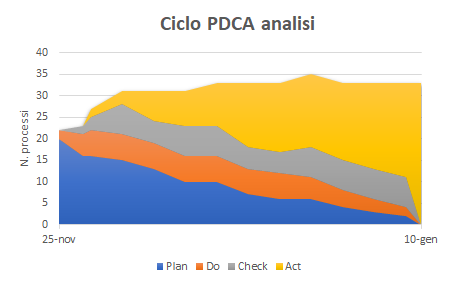
\includegraphics[scale=1]{Img/Ciclo_PDCA}
	\caption{Grafico del metodo PDCA, fase di Analisi}\label{immagine:pdca analisi}
\end{figure}
Dal grafico possiamo estrapolare che:
\begin{itemize}
	\item Alcuni dei processi pianificati hanno subito mutamenti, dovuti ad errori di pianificazione dati dalla poca esperienza del gruppo di lavoro;
	\item Il gruppo ha reso l'avanzamento dei processi omogeneo, nonostante alcuni rallentamenti dovuti alla sovrapposizione di impegni personali e universitari dei componenti del gruppo con la realizzazione del progetto. Nel complesso si vede come l'omogeneità è stata abbastanza rispettata.
\end{itemize}

\subsubsection{Revisione di Progettazione}

\paragraph{Consolidamento dei requisiti}\MiniSpazio
\renewcommand{\arraystretch}{1.5}
\begin{table}[H]
	\begin{center}
		\begin{tabular}{|c|c|p{6.8cm}|}
			\hline
			\rowcolor{title_row}
			\textbf{\color{title_text}{Processo}} & \textbf{\color{title_text}{Livello di maturità}} & \textbf{\color{title_text}{Considerazioni}} \\
			\hline
			{Pianificazione e controllo} & {3} & {Gestito con l'ausilio di nTask, ha permesso di rispettare le scadenze previste.}\\	
			\hline
			{Gestione dei rischi} & {1} & {Non si sono verificate situazioni di rischio.}\\	
			\hline
			{Gestione dei test} & {0} & {Verrà istanziato una volta presente la necessità di definire e condurre dei test.}\\	
			\hline
			{Versionamento e build} & {0} & {Verrà istanziato una volta presente la necessità di versionare il prodotto software.}\\	
			\hline
		\end{tabular}
		\caption[Maturità dei processi, Consolidamento]{Maturità dei processi e considerazioni}	
		\label{tabella: considerazioni sulla maturità dei processi raggiunta}
	\end{center}
\end{table}


Il grafico rappresentante l'applicazione del metodo PDCA nella fase di Consolidamento dei requisiti è:
\begin{figure} [H]
	\centering
	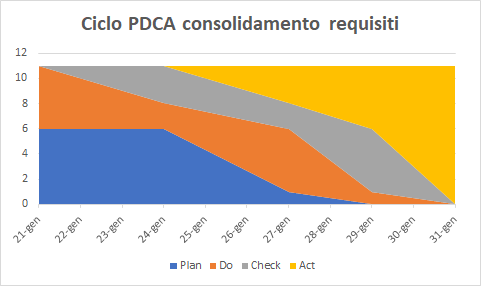
\includegraphics[scale=1]{Img/Ciclo_PDCA_consolidamento_requisiti}
	\caption{Grafico del metodo PDCA, fase di Consolidamento dei requisiti}\label{}
\end{figure}
Dal grafico possiamo estrapolare che:
\begin{itemize}
	\item Trattandosi di un periodo relativamente breve (10 giorni), piccole variazioni nel numero di attività risultano in grossi cambiamenti grafici;
	\item Le attività in Plan sono state esaurite prima del termine del periodo, mentre quelle in Check e Act hanno avuto una permanenza maggiore; ciò è dovuto ad un numero di modifiche ai documenti relativamente basso ma di grande importanza e profondità (soprattutto per quanto riguarda il consolidamento del \emph{Piano di Qualifica}), che quindi hanno richiesto periodi di Check e Act prolungati.
\end{itemize}

\pagebreak
\paragraph{Progettazione architetturale}\MiniSpazio
\renewcommand{\arraystretch}{1.5}
\begin{table}[H]
	\begin{center}
		\begin{tabular}{|c|c|p{6.8cm}|}
			\hline
			\rowcolor{title_row}
			\textbf{\color{title_text}{Processo}} & \textbf{\color{title_text}{Livello di maturità}} & \textbf{\color{title_text}{Considerazioni}} \\
			\hline
			{Pianificazione e controllo} & {3} & {Ha permesso di rispettare le scadenze previste.}\\	
			\hline
			{Gestione dei rischi} & {1} & {Si è dimostrato poco stabile al verificarsi di 3 situazioni di rischio (malattia di membri del gruppo), comportando una ridefinizione degli obiettivi per il periodo.}\\	
			\hline
			{Gestione dei test} & {1} & {Sono stati pianificati i primi test di sistema, le cui specifiche tuttavia rimangono da definire.}\\	
			\hline
			{Versionamento e build} & {1} & {Parzialmente automatizzato con l'utilizzo dello strumento \gl{Travis}.}\\	
			\hline
		\end{tabular}
		\caption[Maturità dei processi, Progettazione Architetturale]{Maturità dei processi e considerazioni}	
		\label{tabella: considerazioni sulla maturità dei processi raggiunta pa}
	\end{center}
\end{table}
\renewcommand{\arraystretch}{1}
Il grafico rappresentante l'applicazione del metodo PDCA nella fase di Progettazione architetturale è:
\begin{figure} [H]
	\centering
	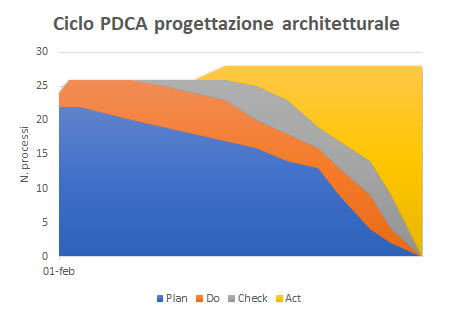
\includegraphics[scale=1]{Img/Ciclo_PDCA_progettazione_architetturale}
	\caption{Grafico del metodo PDCA, fase di Progettazione architetturale}\label{}
\end{figure}
Dal grafico possiamo estrapolare che:
\begin{itemize}
	\item Si nota uno stallo nell'esecuzione delle attività nella prima metà del periodo, dovuto principalmente, come previsto, alla sovrapposizione degli impegni universitari dei vari membri del gruppo. A questo si sono aggiunte le situazioni di rischio verificatesi, comportando ulteriori ritardi;
	\item Verso al fine del periodo si nota un rapido decremento delle attività in Do e Check, dovuto ad uno sforzo maggiorato per compensare i ritardi dovuti alle situazioni di rischio verificatesi.
\end{itemize}

\subsubsection{Revisione di Qualifica}
\paragraph{Progettazione di dettaglio e codifica} \Spazio
\renewcommand{\arraystretch}{1.5}
\begin{table}[H]
	\begin{center}
		\begin{tabular}{|c|c|p{6.8cm}|}
			\hline
			\rowcolor{title_row}
			\textbf{\color{title_text}{Processo}} & \textbf{\color{title_text}{Livello di maturità}} & \textbf{\color{title_text}{Considerazioni}} \\
			\hline
			{Pianificazione e controllo} & {3} & {Ha permesso di rispettare le scadenze previste.}\\	
			\hline
			{Gestione dei rischi} & {3} & {Si è dimostrato stabile al verificarsi di alcune situazioni di basso rischio, grazie alle istruzione impartite dal \emph{Responsabile di Progetto.}}\\	
			\hline
			{Gestione dei test} & {3} & {Sono stati specificati ed implementati buona parte dei test La copertura dei test di unità a registrato esiti molto positivi.}\\	
			\hline
			{Versionamento e build} & {4} & {Automatizzato il processo tramite \gl{Travis}.} Ogni modifica apportata alla repository di GitHub scaturisce una serie di test sul codice, tenendo traccia dell'esito delle varie build e registrando valori utili per le nostre metriche, come il code coverage.\\	
			\hline
		\end{tabular}
		\caption[Maturità dei processi, Progettazione di dettaglio e codifica]{Maturità dei processi e considerazioni}	
		\label{tabella: considerazioni sulla maturità dei processi raggiunta rq}
	\end{center}
\end{table}
\renewcommand{\arraystretch}{1}
Il grafico rappresentante l'applicazione del metodo PDCA nella fase di Progettazione di dettaglio e codifica è:
\begin{figure} [H]
	\centering
	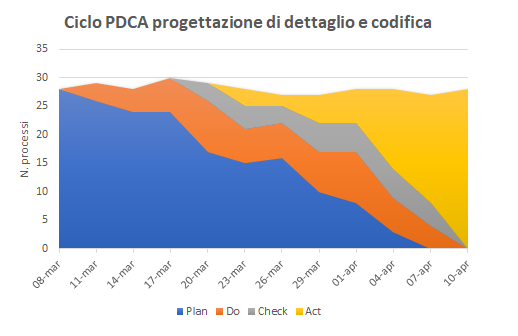
\includegraphics[scale=1]{Img/Ciclo_PDCA_progettazione_dettaglio}
	\caption{Grafico del metodo PDCA, fase di Progettazione di dettaglio e codifica}\label{}
\end{figure}
Dal grafico possiamo estrapolare che:
\begin{itemize}
	\item Si nota una fase iniziale dovuta in maggior parte alla pianificazione delle attività finalizzate all'incremento dei documenti e allo sviluppo dei test;
	\item Il completamento delle attività pianificate comporta delle transizioni tra lo stato Do e lo stato Check che segue un andamento omogeneo, dovuto al fatto che non sono stati registrati scostamenti nelle tempistiche.
\end{itemize}
\newpage

\subsection{Misurazioni}

\subsubsection{Schedule Variance}
Questa metrica è sempre rimasta in linea con il valore accettabile, ma non ha ancora raggiunto quello ottimale.
\begin{figure} [H]
	\centering
	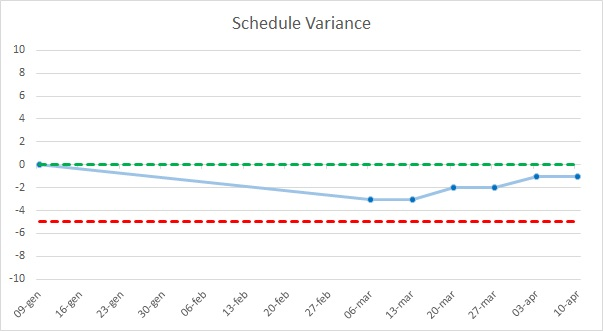
\includegraphics[scale=1]{Img/schedulev}
	\caption{Misurazione Schedule Variance}\label{}
\end{figure}

\subsubsection{Budget Variance}
Questa metrica è sempre rimasta in linea con il valore ottimale.
\begin{figure} [H]
	\centering
	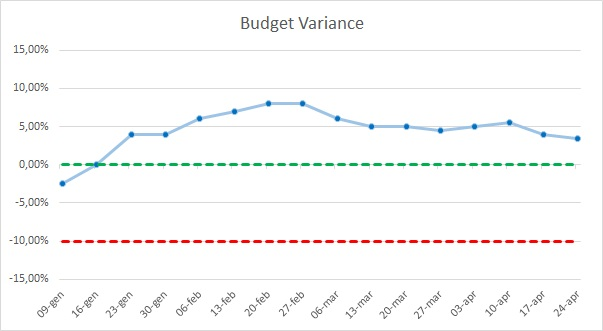
\includegraphics[scale=1]{Img/budgetv}
	\caption{Misurazione Budget Variance}\label{}
\end{figure}

\subsubsection{Numero rischi non previsti}
Questa metrica è sempre rimasta in linea con il valore accettabile.
\begin{figure} [H]
	\centering
	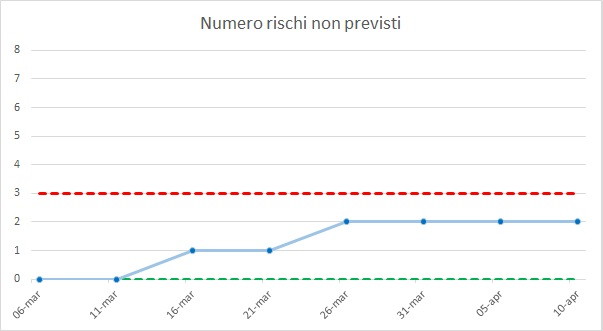
\includegraphics[scale=1]{Img/rischi}
	\caption{Misurazione numero rischi non previsti}\label{}
\end{figure}

\subsubsection{Indisponibilità dei servizi esterni}
Questa metrica è sempre rimasta in linea con il valore ottimale, tranne per il verificarsi dell'indisponibilità del servizio \emph{TravisCI}.
\begin{figure} [H]
	\centering
	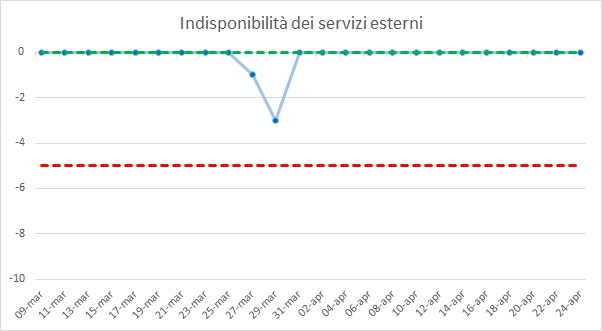
\includegraphics[scale=1]{Img/indisp}
	\caption{Misurazione indisponibilità dei servizi esterni}\label{}
\end{figure}

\subsubsection{Percentuale di test eseguiti}
Questa metrica inizialmente ha registrato dei valori non accettabili, ma con lo sviluppo dei test ha raggiunto un valore accettabile.
\begin{figure} [H]
	\centering
	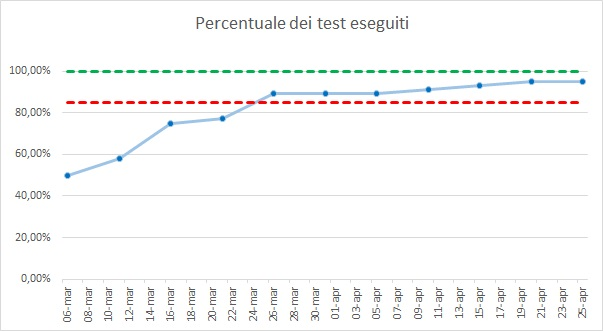
\includegraphics[scale=1]{Img/testEs}
	\caption{Misurazione percentuale di test eseguiti}\label{}
\end{figure}

\subsubsection{Percentuale test case passati}
Questa metrica ha quasi raggiunto un valore ottimale.
\begin{figure} [H]
	\centering
	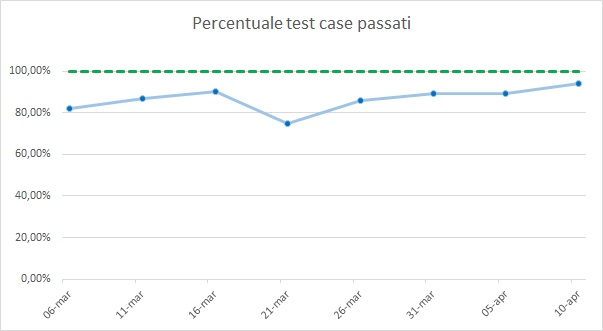
\includegraphics[scale=1]{Img/testPas}
	\caption{Misurazione percentuale test case passati}\label{}
\end{figure}

\subsubsection{Percentuale test case falliti}
Questa metrica ha quasi raggiunto un valore ottimale.
\begin{figure} [H]
	\centering
	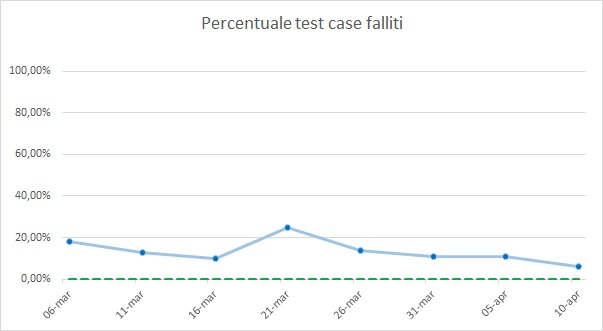
\includegraphics[scale=1]{Img/testNoPas}
	\caption{Misurazione percentuale test case falliti}\label{}
\end{figure}

\subsubsection{Code coverage}
Questa metrica inizialmente ha registrato dei valori non accettabili, ma con lo sviluppo dei test ha raggiunto un valore quasi ottimale.
\begin{figure} [H]
	\centering
	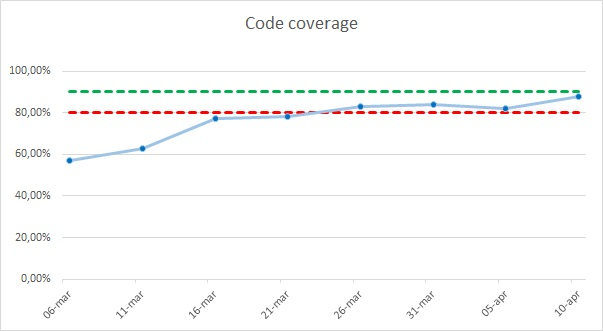
\includegraphics[scale=1]{Img/CC}
	\caption{Misurazione code coverage}\label{}
\end{figure}

\subsubsection{Tempo medio necessario al team per risolvere un errore}
Questa metrica è sempre rimasta in linea con un valore ottimale, tranne in un'occasione causata da un errore consistente.
\begin{figure} [H]
	\centering
	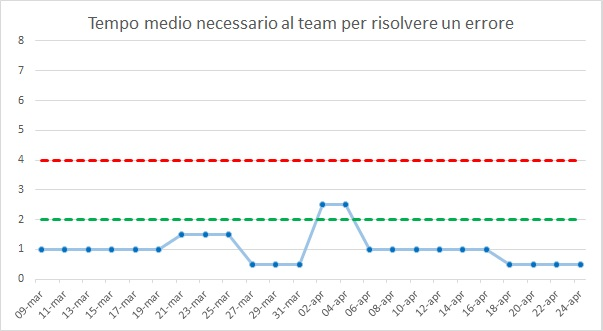
\includegraphics[scale=1]{Img/risErr}
	\caption{Misurazione tempo medio necessario per risolvere un errore}\label{}
\end{figure}

\subsubsection{Efficienza nella progettazione dei test}
Tranne per la fase di sviluppo dei test iniziale, ha sempre registrato un valore ottimale.
\begin{figure} [H]
	\centering
	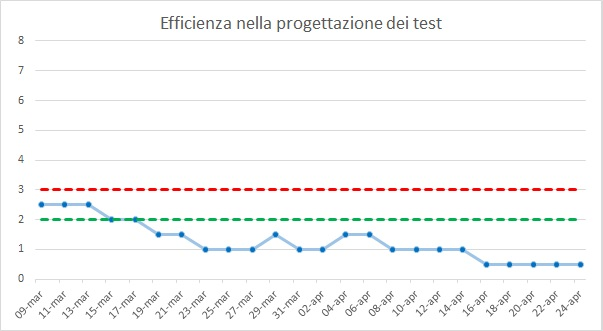
\includegraphics[scale=1]{Img/progTest}
	\caption{Misurazione efficienza nella progettazione dei test}\label{}
\end{figure}

\subsubsection{Percentuale di errori corretti}
La presenza di vari errori ha fatto registrare dei valori non accettabili, ma grazie al lavoro dei \emph{Verificatori} questi sono stati corretti, raggiungendo un valore ottimale per questa metrica.
\begin{figure} [H]
	\centering
	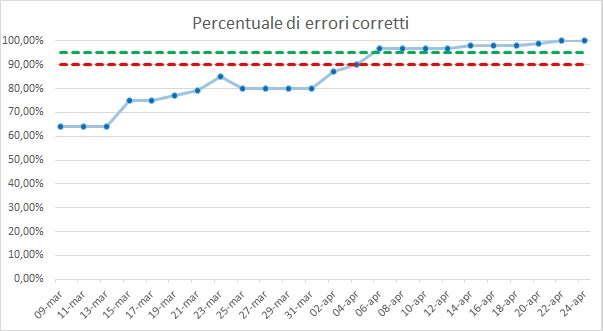
\includegraphics[scale=1]{Img/errCorr}
	\caption{Misurazione percentuale di errori corretti}\label{}
\end{figure}

\subsubsection{Media commit a settimana}
Il lavoro costante del gruppo ha permesso di registrare dei valori accettabili, a volte anche ottimali, per questa metrica.
\begin{figure} [H]
	\centering
	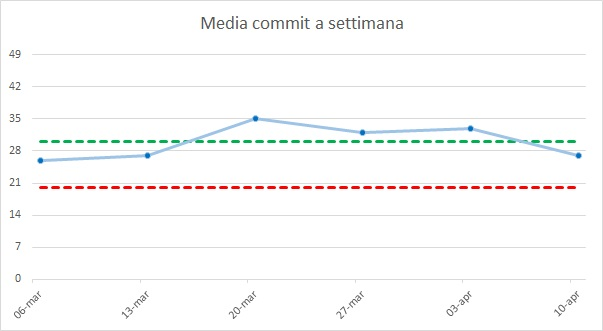
\includegraphics[scale=1]{Img/commit}
	\caption{Misurazione media commit a settimana}\label{}
\end{figure}

\subsubsection{Media build Travis a settimana}
Il lavoro costante del gruppo ha permesso di registrare dei valori accettabili, a volte anche ottimali, per questa metrica.
\begin{figure} [H]
	\centering
	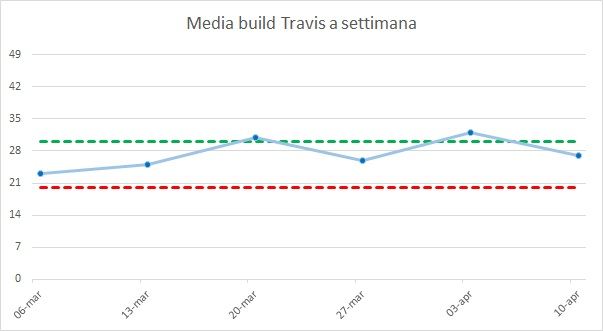
\includegraphics[scale=1]{Img/build}
	\caption{Misurazione media build Travis a settimana}\label{}
\end{figure}

\subsubsection{Percentuale build Travis superate}
La presenza di vari errori ha fatto registrare dei valori non accettabili inizialmente, ma una volta corrette queste criticità questa metrica ha raggiunto un valore accettabile.
\begin{figure} [H]
	\centering
	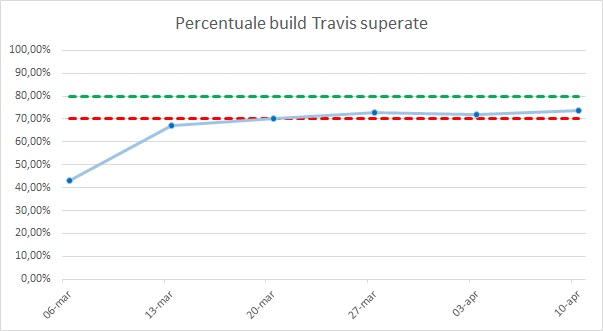
\includegraphics[scale=1]{Img/buildPass}
	\caption{Misurazione percentuale build Travis superate}\label{}
\end{figure}

\subsubsection{Gunning fog index}
Tutti gli indici Gunning fox dei documenti rientrano nei vincoli dati. Per questo motivo i documenti redatti hanno raggiunto la leggibilità desiderata.
\begin{figure} [H]
	\centering
	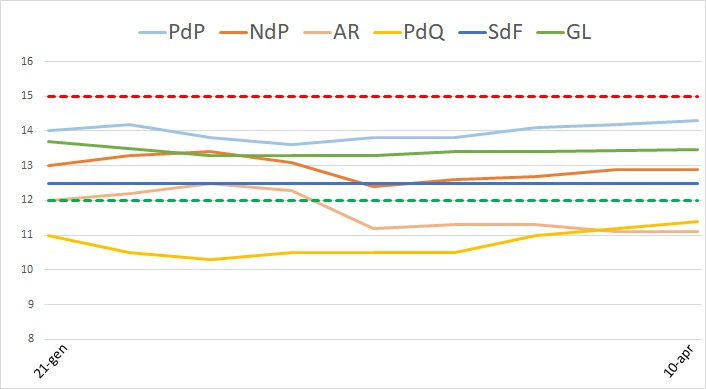
\includegraphics[scale=1]{Img/fog}
	\caption{Misurazione Gunning fog index}\label{}
\end{figure}

\subsubsection{Indice di Gulpease}
Tutti gli indici Gulpease dei documenti rientrano nei vincoli dati. Per questo motivo i documenti redatti hanno raggiunto la leggibilità desiderata.
\begin{figure} [H]
	\centering
	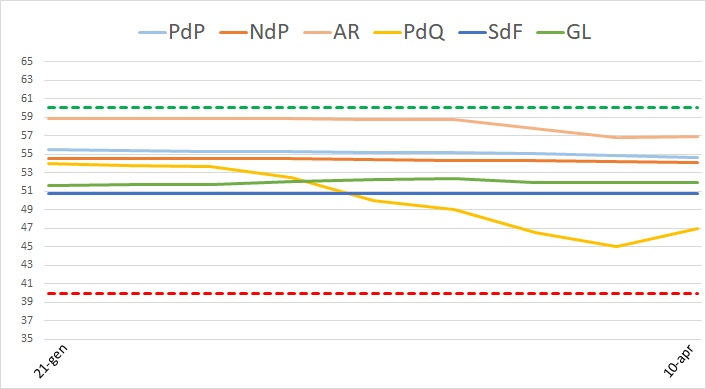
\includegraphics[scale=1]{Img/gulp}
	\caption{Misurazione indice di Gulpease}\label{}
\end{figure}

\subsubsection{Numero di errori grammaticali}
Grazie le procedura di verifica e correzione attuate e all'ausilio dello strumento di controllo ortografico integrato in \gl{TexStudio}, il numero di errori ortografici per ogni documento ha raggiunto il valore ottimale di 0.
\begin{figure} [H]
	\centering
	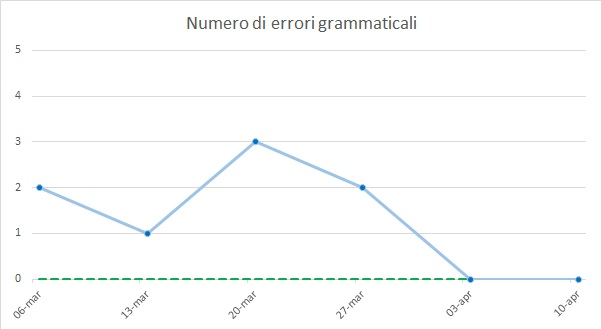
\includegraphics[scale=1]{Img/gramm}
	\caption{Misurazione numero di errori grammaticali}\label{}
\end{figure}

\subsubsection{Functional Implementation Completeness}
La scarsa copertura delle funzionalità inizialmente ha fatto registrare valori non accettabili, ma grazie al lavoro del team questa metrica ha raggiunto un valore accettabile, anche se non ancora ottimale.
\begin{figure} [H]
	\centering
	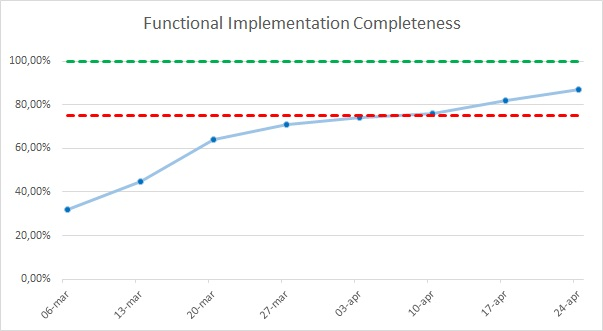
\includegraphics[scale=1]{Img/FIC}
	\caption{Misurazione Functional Implementation Completeness}\label{}
\end{figure}

\subsubsection{Average Functional Implementation Correctness}
La presenza di alcune criticità inizialmente ha fatto registrare valori non accettabili, ma grazie al lavoro del team questa metrica ha raggiunto un valore accettabile, anche se non ancora ottimale.
\begin{figure} [H]
	\centering
	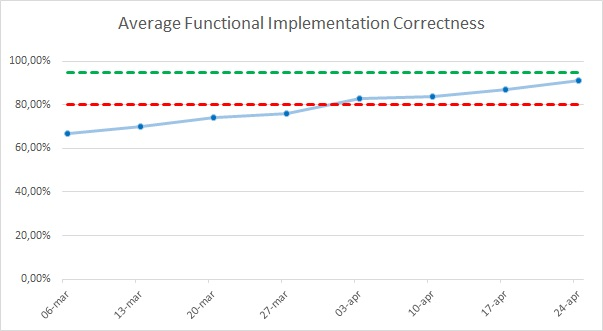
\includegraphics[scale=1]{Img/AFIC}
	\caption{Misurazione Average Functional Implementation Correctness}\label{}
\end{figure}

\subsubsection{Tempo di risposta}
Il valore di questa metrica è sempre rimasto in linea con il valore ottimale.
\begin{figure} [H]
	\centering
	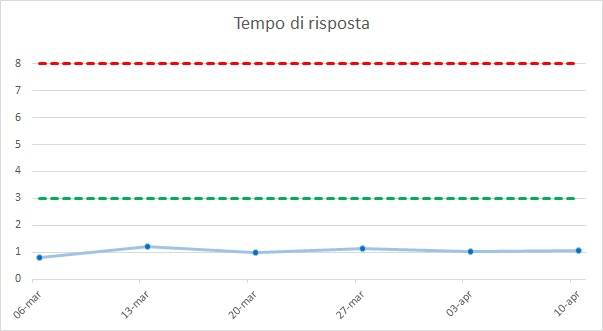
\includegraphics[scale=1]{Img/risp}
	\caption{Misurazione tempo di risposta}\label{}
\end{figure}

\subsubsection{Average Learning Time}
Il valore di questa metrica è sempre rimasto in linea con il valore accettabile.
\begin{figure} [H]
	\centering
	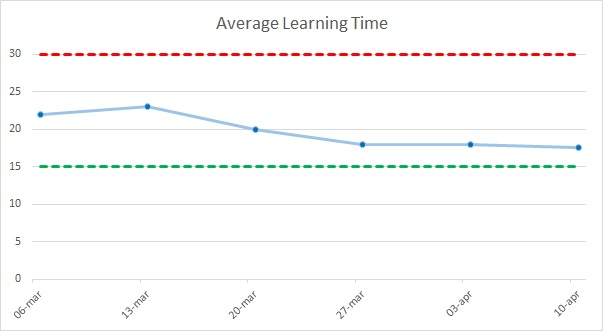
\includegraphics[scale=1]{Img/ALT}
	\caption{Misurazione Average Learning Time}\label{}
\end{figure}

\subsubsection{Failure Density}
La presenza di alcune criticità iniziali ha fatto registrare valori non accettabili, ma grazie al lavoro del team questa metrica ha raggiunto un valore accettabile, anche se non ancora ottimale.
\begin{figure} [H]
	\centering
	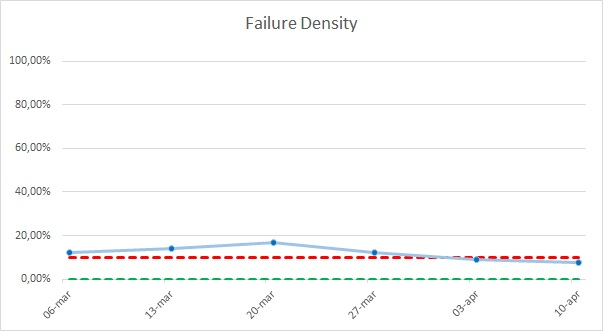
\includegraphics[scale=1]{Img/FD}
	\caption{Misurazione Failure Density}\label{}
\end{figure}

\subsubsection{Operazioni con gestione errori}
Inizialmente abbiamo registrato dei valori non accettabili a causa della scarsa gestione degli errori, ma grazie allo sviluppo dei test siamo riusciti ad ottenere un valore accettabile per questa metrica.
\begin{figure} [H]
	\centering
	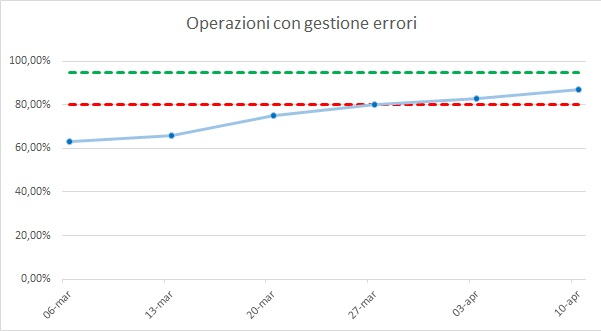
\includegraphics[scale=1]{Img/blocco}
	\caption{Misurazione }\label{}
\end{figure}

\subsubsection{Failure Analysis}
Il valore di questa metrica è sempre rimasto in linea con il valore accettabile.
\begin{figure} [H]
	\centering
	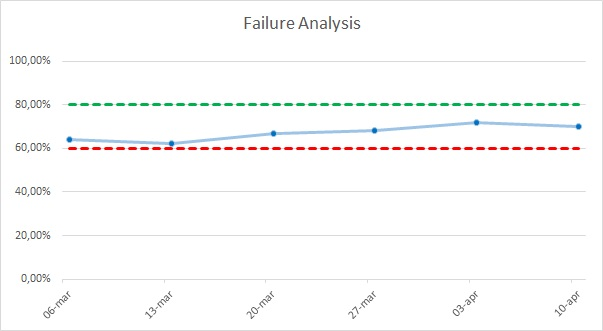
\includegraphics[scale=1]{Img/FA}
	\caption{Misurazione Failure Analysis}\label{}
\end{figure}

\subsubsection{Comment Ratio}
La presenza di pochi commenti nel codice inizialmente ha fatto registrare dei valori non accettabili, ma con il lavoro del team questa metrica ha raggiunto un valore accettabile.
\begin{figure} [H]
	\centering
	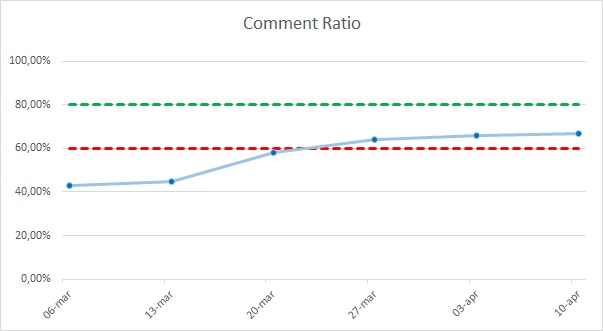
\includegraphics[scale=1]{Img/CR}
	\caption{Misurazione Comment Ratio}\label{}
\end{figure}
\newpage

\newsection{Specifica dei test}
\subsection{Test di accettazione}
\normalsize
\renewcommand{\arraystretch}{1}
\begin{longtable}{|C{2.5cm}|C{13cm}|}
	\hline
	\rowcolor{title_row}
	\textbf{\color{title_text}{Test}} & \textbf{\color{title_text}{Specifica}}  \\
	\hline
	\endhead
{TA-1} &
\begin{itemize}
	\item \textbf{Progettazione}: verifica che il sistema permetta di leggere la definizione di una rete Bayesiana importando un file in formato JSON;
	\item \textbf{Caso}: 
		\begin{itemize}
			\item \textbf{Input}: file JSON con la definizione di rete;
			\item \textbf{Risultato atteso}: il sistema importa la definizione della rete mostrandone il contenuto.
		\end{itemize}
	\item \textbf{Procedura}:
		\begin{itemize}
			\item L'utente crea un nuovo 7DOS panel;
			\item L'utente si posiziona sulla scheda di \emph{"Edit"};
			\item L'utente si posiziona sul \emph{"JSON import"} panel;
			\item L'utente preme il pulsante per importare un file JSON;
			\item L'utente seleziona il file da importare;
			\item Conferma la selezione del file.
		\end{itemize} 
\end{itemize} \\
\hline

{TA-2} &
\begin{itemize}
	\item \textbf{Progettazione}: verifica che il sistema permetta la gestione della connessione tra i nodi della rete ed il flusso di dati;
	\item \textbf{Caso}: 
	\begin{itemize}
		\item \textbf{Input}:
		\item \textbf{Risultato atteso}: il sistema effettua la connessione tra flusso dati e nodi della rete.
	\end{itemize}
	\item \textbf{Procedura}:
	\begin{itemize}
		\item L'utente si posiziona sulla scheda di \emph{"Edit"};
		\item L'utente si posiziona sul \emph{"Network"} panel;
		\item L'utente seleziona il flusso di dati da monitorare.
	\end{itemize} 
\end{itemize} \\
 \hline
{TA-2.1} &
\begin{itemize}
	\item \textbf{Progettazione}: verifica che il sistema permetta di connettere un nodo della rete al flusso di dati;
	\item \textbf{Caso}: 
	\begin{itemize}
		\item \textbf{Input}: 
		\item \textbf{Risultato atteso}: il sistema connette il nodo selezionato e lo monitora rispetto al flusso dati.
	\end{itemize}
	\item \textbf{Procedura}:
	\begin{itemize}
		\item L'utente si posiziona sulla scheda di \emph{"Edit"};
		\item L'utente si posiziona sul \emph{"Network"} panel;
		\item L'utente seleziona il nodo da monitorare rispetto al flusso di dati.
	\end{itemize} 
\end{itemize} \\
\hline
{TA-2.2} &
\begin{itemize}
	\item \textbf{Progettazione}: verifica che il sistema permetta di disconnettere un nodo della rete al flusso di dati;
	\item \textbf{Caso}: 
	\begin{itemize}
		\item \textbf{Input}:
		\item \textbf{Risultato atteso}: il sistema disconnette il nodo selezionato.
	\end{itemize}
	\item \textbf{Procedura}:
	\begin{itemize}
		\item L'utente si posiziona sulla scheda di \emph{"Edit"};
		\item L'utente si posiziona sul \emph{"Network"} panel;
		\item L'utente deseleziona il nodo da monitorare rispetto al flusso di dati.
	\end{itemize} 
\end{itemize} \\
\hline
{TA-2.3} &
\begin{itemize}
	\item \textbf{Progettazione}: verifica che il sistema permetta di modificare un nodo della rete connesso al flusso di dati;
	\item \textbf{Caso}: 
	\begin{itemize}
		\item \textbf{Input}: 
		\item \textbf{Risultato atteso}: il sistema apporta le modifiche richieste.
	\end{itemize}
	\item \textbf{Procedura}:
	\begin{itemize}
		\item L'utente si posiziona sulla scheda di \emph{"Edit"};
		\item L'utente si posiziona sul \emph{"Network"} panel;
		\item L'utente modifica il nodo da monitorare rispetto al flusso di dati.
	\end{itemize} 
\end{itemize}\\
\hline
{TA-3} &
\begin{itemize}
	\item \textbf{Progettazione}: verifica che il sistema permetta di applicare il
	ricalcolo delle probabilità della rete
	secondo regole temporali stabilite dall'utente.;
	\item \textbf{Caso}: 
	\begin{itemize}
		\item \textbf{Input}: 
		\item \textbf{Risultato atteso}: il sistema effettua il ricalcolo delle probabilità della rete aggiornandone lo stato dei nodi.
	\end{itemize}
	\item \textbf{Procedura}:
	\begin{itemize}
		\item Il sistema legge i dati provenienti dal flusso;
		\item Il sistema li elabora calcolando le probabilità dei nodi;
		\item Il sistema aggiorna lo stato dei nodi.
	\end{itemize} 
\end{itemize}\\
\hline
{TA-3.1} &
\begin{itemize}
	\item \textbf{Progettazione}: verifica che il sistema permetta all'utente di modificare le regole temporali per effettuare il ricalcolo delle probabilità della rete;
	\item \textbf{Caso}: 
	\begin{itemize}
		\item \textbf{Input}: 
		\item \textbf{Risultato atteso}: il sistema apporta le modifiche richieste alle regole temporali per il ricalcolo delle probabilità.
	\end{itemize}
	\item \textbf{Procedura}:
	\begin{itemize}
		\item L'utente si posiziona sulla scheda di \emph{"Edit"};
		\item L'utente si posiziona sul \emph{"Network"} panel;
		\item L'utente modifica le regole temporali per il ricalcolo delle probabilità della rete.
	\end{itemize} 
\end{itemize} \\
\hline
{TA-4} &
\begin{itemize}
	\item \textbf{Progettazione}: verifica che il sistema permetta di fornire nuovi dati a Grafana derivati dai nodi della rete non direttamente collegati al flusso di
	dati;
	\item \textbf{Caso}: 
	\begin{itemize}
		\item \textbf{Input}:
		\item \textbf{Risultato atteso}: il sistema elabora i dati proveniente dai nodi non connessi al flusso.
	\end{itemize}
	\item \textbf{Procedura}:
	\begin{itemize}
		\item Il sistema legge i dati in ingresso dal flusso;
		\item Il sistema elabora i dati;
		\item Il sistema usa i risultati ottenuti per calcolare le probabilità dei nodi non connessi.
	\end{itemize} 
\end{itemize}\\
\hline
{TA-4.1} &
\begin{itemize}
	\item \textbf{Progettazione}: verifica che il sistema permetta l'aggiornamento dei dati secondo una frequenza stabilita dall'utente;
	\item \textbf{Caso}: 
	\begin{itemize}
		\item \textbf{Input}:
		\item \textbf{Risultato atteso}: il sistema effettua l'aggiornamento costante dei dati.
	\end{itemize}
	\item \textbf{Procedura}:
	\begin{itemize}
		\item Il sistema, dopo un tempo predefinito, legge nuovi dati in ingresso;
		\item Il sistema elabora i nuovi dati.
	\end{itemize} 
\end{itemize} \\
\hline
{TA-5} &
\begin{itemize}
	\item \textbf{Progettazione}: verifica che il sistema permetta di leggere i dati provenienti dal flusso ed elaborarli, visualizzandone il risultato attraverso un grafico;
	\item \textbf{Caso}: 
	\begin{itemize}
		\item \textbf{Input}: flusso di dati;
		\item \textbf{Risultato atteso}: grafico derivato dall'elaborazione dei dati.
	\end{itemize}
	\item \textbf{Procedura}:
	\begin{itemize}
		\item Il sistema legge i dati in ingresso dal flusso;
		\item Il sistema elabora i dati ricevuti;
		\item Il sistema costruisce un grafico sulla base dei risultati ottenuti.
	\end{itemize} 
\end{itemize} \\
\hline

{TA-5.1} &
\begin{itemize}
	\item \textbf{Progettazione}: verifica che il sistema aggiorni i dati presenti nel grafico in base alla frequenza stabilita dall'utente;
	\item \textbf{Caso}: 
	\begin{itemize}
		\item \textbf{Input}: nuovi dati dal flusso;
		\item \textbf{Risultato atteso}: il sistema aggiorna i dati nel grafico.
	\end{itemize}
	\item \textbf{Procedura}:
	\begin{itemize}
		\item Il sistema legge i nuovi dati proveniente dal flusso, in base alla frequenza stabilita;
		\item Il sistema effettua il ricalcolo delle probabilità della rete aggiornando lo stato dei nodi, in base alla frequenza stabilita;
		\item Il sistema elabora i risultati e li mostra attraverso un grafico.
	\end{itemize} 
\end{itemize} \\
\hline
{TA-5.2} &
\begin{itemize}
	\item \textbf{Progettazione}: verifica che il sistema permetta all'utente di creare un nuovo panel;
	\item \textbf{Caso}: 
	\begin{itemize}
		\item \textbf{Input}:
		\item \textbf{Risultato atteso}: il sistema crea il nuovo panel e lo mostra all'interno della dashboard..
	\end{itemize}
	\item \textbf{Procedura}:
	\begin{itemize}
		\item L'utente si posiziona all'interno di una dashboard;
		\item L'utente clicca sulla voce \emph{add panel};
		\item L'utente sceglie la tipologia di panel da creare.
	\end{itemize} 
\end{itemize} \\
\hline
{TA-5.3} &
\begin{itemize}
	\item \textbf{Progettazione}: verifica che il sistema permetta all'utente di spostare un panel all'interno della dashboard;
	\item \textbf{Caso}: 
	\begin{itemize}
		\item \textbf{Input}:
		\item \textbf{Risultato atteso}: il sistema sposta panel nella nuova posizione scelta dall'utente.
	\end{itemize}
	\item \textbf{Procedura}:
	\begin{itemize}
		\item L'utente si posiziona all'interno di una dashboard;
		\item L'utente trascina il panel che vuole spostare nella posizione desiderata.
	\end{itemize} 
\end{itemize} \\
\hline
{TA-5.4} &
\begin{itemize}
	\item \textbf{Progettazione}: verifica che il sistema permetta all'utente di cancellare un panel all'interno della dashboard;
	\item \textbf{Caso}: 
	\begin{itemize}
		\item \textbf{Input}: ;
		\item \textbf{Risultato atteso}: il sistema cancella panel scelto dall'utente.
	\end{itemize}
	\item \textbf{Procedura}:
	\begin{itemize}
		\item L'utente si posiziona all'interno di una dashboard;
		\item L'utente clicca sull'intestazione del panel;
		\item L'utente seleziona la voce \emph{"Remove"};
		\item Conferma l'eliminazione del panel.
	\end{itemize} 
\end{itemize} \\
\hline
{TA-5.5} &
\begin{itemize}
	\item \textbf{Progettazione}: verifica che il sistema permetta all'utente di minimizzare un panel;
	\item \textbf{Caso}: 
	\begin{itemize}
		\item \textbf{Input}: ;
		\item \textbf{Risultato atteso}: il sistema modifica la dimensione del panel come scelto dall'utente.
	\end{itemize}
	\item \textbf{Procedura}:
	\begin{itemize}
		\item L'utente si posiziona all'interno di una dashboard;
		\item L'utente si posiziona sull'angolo in basso a destra del panel;
		\item L'utente modifica minimizza il panel.
	\end{itemize} 
\end{itemize} \\
\hline
{TA-5.6} &
\begin{itemize}
	\item \textbf{Progettazione}: verifica che il sistema permetta all'utente configurare un panel dopo la sua creazione;
	\item \textbf{Caso}: 
	\begin{itemize}
		\item \textbf{Input}: ;
		\item \textbf{Risultato atteso}: il sistema configura le opzioni del panel come stabilito dall'utente.
	\end{itemize}
	\item \textbf{Procedura}:
	\begin{itemize}
		\item L'utente si posiziona all'interno di una dashboard;
		\item L'utente configura le opzioni del panel come desidera.
	\end{itemize} 
\end{itemize} \\
\hline
{TA-5.7} &
\begin{itemize}
	\item \textbf{Progettazione}: verifica che il sistema permetta all'utente di modificare un panel all'interno della dashboard;
	\item \textbf{Caso}: 
	\begin{itemize}
		\item \textbf{Input}: ;
		\item \textbf{Risultato atteso}: il sistema modifica le opzioni del panel come stabilito dall'utente.
	\end{itemize}
	\item \textbf{Procedura}:
	\begin{itemize}
		\item L'utente si posiziona all'interno di una dashboard;
		\item L'utente modifica le opzioni del panel come desidera.
	\end{itemize} 
\end{itemize} \\
\hline
{TA-6} &
\begin{itemize}
	\item \textbf{Progettazione}: verifica che il sistema permetta all'utente di definire alert in base a livelli di soglia raggiunti dai nodi non collegati al flusso dei dati;
	\item \textbf{Caso}: 
	\begin{itemize}
		\item \textbf{Input}: ;
		\item \textbf{Risultato atteso}: il sistema crea un nuovo alert.
	\end{itemize}
	\item \textbf{Procedura}:
	\begin{itemize}
		\item L'utente si posiziona all'interno di un panel di tipo \emph{graph};
		\item L'utente si posiziona sulla schermata di \emph{edit};
		\item L'utente si posiziona sulla scheda \emph{"Alert"};
		\item L'utente clicca sul pulsante \emph{"Create alert"}.
	\end{itemize} 
\end{itemize} \\
\hline
{TA-6.1} &
\begin{itemize}
	\item \textbf{Progettazione}: verifica che il sistema permetta all'utente di configurare i parametri di un alert;
	\item \textbf{Caso}: 
	\begin{itemize}
		\item \textbf{Input}: ;
		\item \textbf{Risultato atteso}: il sistema configura i parametri dell'alert.
	\end{itemize}
	\item \textbf{Procedura}:
	\begin{itemize}
		\item L'utente si posiziona sulla scheda \emph{"Alert"};
		\item L'utente seleziona l'alert da configurare;
		\item L'utente configura i parametri come desidera.
	\end{itemize} 
\end{itemize} \\
\hline
{TA-6.2} &
\begin{itemize}
	\item \textbf{Progettazione}: verifica che il sistema permetta all'utente di impostare il modo in cui viene notificata l'attivazione di un alert;
	\item \textbf{Caso}: 
	\begin{itemize}
		\item \textbf{Input}: ;
		\item \textbf{Risultato atteso}: il sistema imposta il sistema di notifica dell'alert.
	\end{itemize}
	\item \textbf{Procedura}:
	\begin{itemize}
		\item L'utente si posiziona sulla scheda \emph{"Alert"};
		\item L'utente seleziona l'alert da configurare;
		\item L'utente imposta come deve venire notificata l'attivazione dell'alert. 
	\end{itemize} 
\end{itemize} \\
\hline
{TA-7} &
\begin{itemize}
	\item \textbf{Progettazione}: verifica che il sistema permetta di disegnare una rete Bayesiana con un editor grafico specializzato;
	\item \textbf{Caso}: 
	\begin{itemize}
		\item \textbf{Input}:
		\item \textbf{Risultato atteso}: la rete Bayesiana è stata disegnata.
	\end{itemize}
	\item \textbf{Procedura}:
	\begin{itemize}
		\item L'utente avvia l'editor grafico;
		\item L'utente inizia a disegnare una rete Bayesiana;
	\end{itemize} 
\end{itemize} \\
\hline
{TA-7.1} &
\begin{itemize}
	\item \textbf{Progettazione}: verifica che il sistema permetta di creare un nuovo nodo della rete;
	\item \textbf{Caso}: 
	\begin{itemize}
		\item \textbf{Input}:
		\item \textbf{Risultato atteso}: il nuovo della rete è stato creato.
	\end{itemize}
	\item \textbf{Procedura}:
	\begin{itemize}
		\item L'utente preme il pulsante \emph{add node};
		\item L'utente sceglie la posizione in cui crearlo.
	\end{itemize} 
\end{itemize} \\
\hline
{TA-7.2} &
\begin{itemize}
	\item \textbf{Progettazione}: verifica che il sistema permetta di modificare i parametri di un nodo della rete;
	\item \textbf{Caso}: 
	\begin{itemize}
		\item \textbf{Input}:
		\item \textbf{Risultato atteso}: i parametri del nodo vengono modificati.
	\end{itemize}
	\item \textbf{Procedura}:
	\begin{itemize}
		\item L'utente si posiziona nelle impostazioni del nodo;
		\item L'utente modifica i parametri secondo le sue preferenze;
		\item L'utente conferma le modifiche.
	\end{itemize} 
\end{itemize} \\
\hline
{TA-7.3} &
\begin{itemize}
	\item \textbf{Progettazione}: verifica che il sistema permetta di creare un collegamento tra due nodi della rete;
	\item \textbf{Caso}: 
	\begin{itemize}
		\item \textbf{Input}: 
		\item \textbf{Risultato atteso}: il nuovo collegamento viene creato.
	\end{itemize}
	\item \textbf{Procedura}:
	\begin{itemize}
		\item L'utente preme il pulsante \emph{"add link"};
		\item L'utente sceglie i nodi da collegare.
	\end{itemize} 
\end{itemize} \\
\hline
{TA-7.4} &
\begin{itemize}
	\item \textbf{Progettazione}: verifica che il sistema permetta di eliminare un collegamento tra due nodi della rete;
	\item \textbf{Caso}: 
	\begin{itemize}
		\item \textbf{Input}: 
		\item \textbf{Risultato atteso}: il collegamento viene eliminato.
	\end{itemize}
	\item \textbf{Procedura}:
	\begin{itemize}
		\item L'utente preme il pulsante \emph{"remove link"};
		\item L'utente sceglie il collegamento da rimuovere.
	\end{itemize} 
\end{itemize}\\
\hline
{TA-7.5} &
\begin{itemize}
	\item \textbf{Progettazione}: verifica che il sistema permetta di salvare la rete realizzata su un file JSON;
	\item \textbf{Caso}: 
	\begin{itemize}
		\item \textbf{Input}:
		\item \textbf{Risultato atteso}: il file JSON con la definizione della rete viene salvato.
	\end{itemize}
	\item \textbf{Procedura}:
	\begin{itemize}
		\item L'utente preme il pulsante \emph{"save network"};
		\item L'utente sceglie il percorso in cui salvare il file;
		\item L'utente conferma la scelta.
	\end{itemize} 
\end{itemize} \\
\hline
{TA-7.6} &
\begin{itemize}
	\item \textbf{Progettazione}: verifica che il sistema rilevi e sia in grado di gestire eventuali errori derivati dalla modifica di un nodo;
	\item \textbf{Caso}: 
	\begin{itemize}
		\item \textbf{Input}:
		\item \textbf{Risultato atteso}: il sistema mostra un messaggio di errore.
	\end{itemize}
	\item \textbf{Procedura}:
	\begin{itemize}
		\item L'utente si posiziona nelle impostazioni di un nodo;
		\item L'utente effettua delle modifiche non valide.
	\end{itemize} 
\end{itemize} \\
\hline
{TA-8} &
\begin{itemize}
	\item \textbf{Progettazione}: verifica che il sistema permetta di applicare più reti Bayesiane a diversi oggetti di monitoraggio;
	\item \textbf{Caso}: 
	\begin{itemize}
		\item \textbf{Input}: 
		\item \textbf{Risultato atteso}: il sistema avvia il monitoraggio di diversi oggetti.
	\end{itemize}
	\item \textbf{Procedura}:
	\begin{itemize}
		\item L'utente importa più reti Bayesiane;
		\item L'utente connette le reti a diversi flussi di dati.
	\end{itemize} 
\end{itemize} \\
\hline
{TA-9} &
\begin{itemize}
	\item \textbf{Progettazione}: verifica che il sistema permetta di creare una rete Bayesiana a partire dai dati raccolti
	sul campo;
	\item \textbf{Caso}: 
	\begin{itemize}
		\item \textbf{Input}:
		\item \textbf{Risultato atteso}: il sistema crea une rete Bayesiana.
	\end{itemize}
	\item \textbf{Procedura}:
	\begin{itemize}
		\item Il sistema raccoglie i dati provenienti dal flusso;
		\item Il sistema li elabora per costruire una rete Bayesiana.
	\end{itemize} 
\end{itemize} \\
\hline
{TA-10} &
\begin{itemize}
	\item \textbf{Progettazione}: verifica che il sistema permetta di condividere grafici presenti in una dashboard o in un singolo panel;
	\item \textbf{Caso}: 
	\begin{itemize}
		\item \textbf{Input}: 
		\item \textbf{Risultato atteso}: il sistema condivide il grafico secondo l'opzione scelta dall'utente.
	\end{itemize}
	\item \textbf{Procedura}:
	\begin{itemize}
		\item L'utente si posiziona all'interno di una dashboard;
		\item L'utente seleziona l'opzione \emph{"Share"} relativa alla dashboard o ad un panel.
	\end{itemize} 
\end{itemize}\\
\hline
{TA-10.1} &
\begin{itemize}
	\item \textbf{Progettazione}: verifica che il sistema permetta di visualizzare il link diretto ad una dashboard o ad un
	panel;
	\item \textbf{Caso}: 
	\begin{itemize}
		\item \textbf{Input}: 
		\item \textbf{Risultato atteso}: il sistema mostra il link generato con cui l'utente può effettuare la condivisione.
	\end{itemize}
	\item \textbf{Procedura}:
	\begin{itemize}
		\item L'utente si posiziona all'interno di una dashboard;
		\item L'utente seleziona l'opzione \emph{"Share"} relativa alla dashboard o ad un panel;
		\item L'utente si posiziona sulla scheda \emph{"Link"};
		\item L'utente configura le opzioni per generare il link per la condivisione.
	\end{itemize} 
\end{itemize}\\
\hline
{TA-10.2} &
\begin{itemize}
	\item \textbf{Progettazione}: verifica che il sistema permetta di visualizzare il codice per l'inclusione di un panel in una pagina web;
	\item \textbf{Caso}: 
	\begin{itemize}
		\item \textbf{Input}: 
		\item \textbf{Risultato atteso}: Il sistema mostra il frame generato con cui l'utente può effettuare la condivisione.
	\end{itemize}
	\item \textbf{Procedura}:
	\begin{itemize}
		\item L'utente si posiziona all'interno di una dashboard;
		\item L'utente seleziona l'opzione \emph{"Share"} relativa ad un panel;
		\item L'utente si posiziona sulla scheda \emph{"Embed"};
		\item L'utente configura le opzioni per generare il frame per la condivisione.
	\end{itemize} 
\end{itemize}\\
\hline
{TA-10.4} &
\begin{itemize}
	\item \textbf{Progettazione}: verifica che il sistema permetta di condividere lo snapshot di una dashboard o di un
	panel;
	\item \textbf{Caso}: 
	\begin{itemize}
		\item \textbf{Input}: 
		\item \textbf{Risultato atteso}: il sistema effettua la condivisione dello snapshot.
	\end{itemize}
	\item \textbf{Procedura}:
	\begin{itemize}
		\item L'utente si posiziona all'interno di una dashboard;
		\item L'utente seleziona l'opzione \emph{"Share"} relativa a una dashboard ad un panel;
		\item L'utente si posiziona sulla scheda \emph{"Snapshot"};
		\item L'utente configura le opzioni per la condivisione dello snapshot.
	\end{itemize} 
\end{itemize}\\
\hline
{TA-10.5} &
\begin{itemize}
	\item \textbf{Progettazione}: verifica che il sistema permetta di visualizzare il codice JSON contenente la definizione
	di una dashboard;
	\item \textbf{Caso}: 
	\begin{itemize}
		\item \textbf{Input}: 
		\item \textbf{Risultato atteso}: il sistema mostra il codice JSON con la definizione della dashboard.
	\end{itemize}
	\item \textbf{Procedura}:
	\begin{itemize}
		\item L'utente si posiziona all'interno di una dashboard;
		\item L'utente seleziona l'opzione \emph{"Share dashboard"};
		\item L'utente si posiziona sulla scheda \emph{"Export"};
		\item L'utente clicca sul pulsante per visualizzare il JSON.
	\end{itemize} 
\end{itemize}\\
\hline
{TA-10.6} &
\begin{itemize}
	\item \textbf{Progettazione}: verifica che il sistema permetta di salvare il file JSON contenente la definizione di una
	dashboard;
	\item \textbf{Caso}: 
	\begin{itemize}
		\item \textbf{Input}: 
		\item \textbf{Risultato atteso}: il sistema effettua il salvataggio del codice JSON con la definizione della dashboard.
	\end{itemize}
	\item \textbf{Procedura}:
	\begin{itemize}
		\item L'utente si posiziona all'interno di una dashboard;
		\item L'utente seleziona l'opzione \emph{"Share dashboard"};
		\item L'utente si posiziona sulla scheda \emph{"Export"};
		\item L'utente clicca sul pulsante per salvare il JSON.
	\end{itemize} 
\end{itemize}\\
\hline
\caption{Specifica test di accettazione}
\end{longtable}
\renewcommand{\arraystretch}{1}
\newpage

\subsection{Test di sistema}
\normalsize
\renewcommand{\arraystretch}{1}
\begin{longtable}{|C{2.5cm}|C{13cm}|}
	\hline
	\rowcolor{title_row}
	\textbf{\color{title_text}{Test}} & \textbf{\color{title_text}{Specifica}}  \\
	\hline
	\endhead
	{TS-1} &
\begin{itemize}
	\item \textbf{Progettazione}: verifica che sia possibile e leggere la
	definizione della rete Bayesiana da un file in formato JSON;
	\item \textbf{Caso}: 
	\begin{itemize}
		\item \textbf{Input}: file JSON con la definizione di una rete Bayesiana;
		\item \textbf{Risultato atteso}: il sistema legge il JSON e costruisce la rete.
	\end{itemize}
	\item \textbf{Procedura}:
	\begin{itemize}
		\item L'utente preme il pulsante per importare un file;
		\item L'utente seleziona il file;
		\item L'utente conferma la selezione.
	\end{itemize} 
\end{itemize} \\
	\hline
	{TS-1.1} &
\begin{itemize}
	\item \textbf{Progettazione}: verifica che sia possibile validare un
	file JSON;
	\item \textbf{Caso}: 
	\begin{itemize}
		\item \textbf{Input}: file JSON;
		\item \textbf{Risultato atteso}: il sistema mostra degli errori se il file non è valido.
	\end{itemize}
	\item \textbf{Procedura}:
	\begin{itemize}
		\item L'utente seleziona un JSON da importare;
		\item L'utente conferma la selezione;
		\item Il sistema verifica la validità del file.
	\end{itemize} 
\end{itemize}\\
	\hline
	{TS-2} & 
\begin{itemize}
	\item \textbf{Progettazione}: verifica che sia possibile gestire la
	connessione tra i nodi della rete ai rispettivi flussi di dati;
	\item \textbf{Caso}: 
	\begin{itemize}
		\item \textbf{Input}: 
		\item \textbf{Risultato atteso}: il sistema effettua la connessione tra flusso dati e nodi della rete.
	\end{itemize}
	\item \textbf{Procedura}:
	\begin{itemize}
		\item L'utente si posiziona sul \emph{"Network"} panel;
		\item L'utente seleziona il flusso dati da monitorare.
	\end{itemize} 
\end{itemize} \\
	\hline
	{TS-2.1} &
\begin{itemize}
	\item \textbf{Progettazione}: verifica che sia possibile connettere un
	nodo della rete ad un flusso di dati;
	\item \textbf{Caso}: 
	\begin{itemize}
		\item \textbf{Input}: 
		\item \textbf{Risultato atteso}: il sistema connette il nodo selezionato al flusso dati.
	\end{itemize}
	\item \textbf{Procedura}:
	\begin{itemize}
		\item L'utente si posiziona sul \emph{"Network"} panel;
		\item L'utente sceglie quale nodo monitorare rispetto al flusso dati.
	\end{itemize} 
\end{itemize}	
	 \\
	\hline
	{TS-2.2} &
\begin{itemize}
	\item \textbf{Progettazione}: verifica che sia possibile disconnettere un
	nodo della rete da un flusso di dati.;
	\item \textbf{Caso}: 
	\begin{itemize}
		\item \textbf{Input}: 
		\item \textbf{Risultato atteso}: il sistema disconnette il nodo selezionato dal flusso dati.
	\end{itemize}
	\item \textbf{Procedura}:
	\begin{itemize}
		\item L'utente si posiziona sul \emph{"Network"} panel;
		\item L'utente sceglie quale nodo disconnettere rispetto al flusso dati.
	\end{itemize} 
\end{itemize}
	 \\
	\hline
	{TS-2.3} &
\begin{itemize}
	\item \textbf{Progettazione}: verifica che sia essere possibile modificare il
	flusso di dati connesso ad un nodo;
	\item \textbf{Caso}: 
	\begin{itemize}
		\item \textbf{Input}: 
		\item \textbf{Risultato atteso}: il sistema  seleziona un altro flusso di dati da associare alla rete.
	\end{itemize}
	\item \textbf{Procedura}:
	\begin{itemize}
		\item L'utente si posiziona sul \emph{"Network"} panel;
		\item L'utente modifica la fonte del flusso dati.
	\end{itemize} 
\end{itemize}	
	  \\
	\hline
	{TS-3} & 
\begin{itemize}
	\item \textbf{Progettazione}: verifica che sia possibile applicare il
	ricalcolo delle probabilità della rete secondo regole temporali prestabilite;
	\item \textbf{Caso}: 
	\begin{itemize}
		\item \textbf{Input}: flusso di dati;
		\item \textbf{Risultato atteso}: il sistema effettua il ricalcolo delle probabilità della
		rete aggiornandone lo stato dei nodi.
	\end{itemize}
	\item \textbf{Procedura}:
	\begin{itemize}
		\item Il sistema legge i dati provenienti dal flusso;
		\item Il sistema li elabora calcolando le probabilità dei nodi;
		\item Il sistema aggiorna lo stato dei nodi.
	\end{itemize} 
\end{itemize}	
	\\
	\hline
	{TS-3.1} & 
\begin{itemize}
	\item \textbf{Progettazione}: verifica che sia possibile modificare le
	suddette regole temporali;
	\item \textbf{Caso}: 
	\begin{itemize}
		\item \textbf{Input}: 
		\item \textbf{Risultato atteso}: il sistema apporta le modifiche richieste alle regole temporali per il ricalcolo delle probabilità.
	\end{itemize}
	\item \textbf{Procedura}:
	\begin{itemize}
		\item L'utente si posiziona sulla scheda di \emph{"Edit"};
		\item L'utente si posiziona sul \emph{"Network"} panel;
		\item L'utente modifica le regole temporali per il ricalcolo delle probabilità della rete.
	\end{itemize} 
\end{itemize}
\\
	\hline
	{TS-4} & 
\begin{itemize}
	\item \textbf{Progettazione}: verifica che sia possibile fornire nuovi dati
	al sistema di Grafana derivati dai nodi della rete non collegati al flusso di
	monitoraggio;
	\item \textbf{Caso}: 
	\begin{itemize}
	\item \textbf{Input}:
	\item \textbf{Risultato atteso}: il sistema elabora i dati proveniente dai nodi non connessi al flusso.
	\end{itemize}
	\item \textbf{Procedura}:
	\begin{itemize}
	\item Il sistema legge i dati in ingresso dal flusso;
	\item Il sistema elabora i dati;
	\item Il sistema usa i risultati ottenuti per calcolare le probabilità dei nodi non connessi.
	\end{itemize}
\end{itemize}
	\\
	\hline
	{TS-4.1} & 
\begin{itemize}
	\item \textbf{Progettazione}: verifica che sia possibile aggiornare i dati
	in base alla frequenza stabilita;
	\item \textbf{Caso}: 
	\begin{itemize}
		\item \textbf{Input}:
		\item \textbf{Risultato atteso}: il sistema effettua l'aggiornamento costante dei dati.
	\end{itemize}
	\item \textbf{Procedura}:
	\begin{itemize}
		\item Il sistema, dopo un tempo predefinito, legge nuovi dati in ingresso;
		\item Il sistema elabora i nuovi dati.
	\end{itemize} 
\end{itemize} \\
	\hline
	{TS-5} & 
\begin{itemize}
	\item \textbf{Progettazione}: verifica che i dati siano disponibili al sistema di
	creazione di grafici e dashboard per la loro visualizzazione;
	\item \textbf{Caso}: 
	\begin{itemize}
		\item \textbf{Input}: flusso di dati;
		\item \textbf{Risultato atteso}: grafico derivato dall'elaborazione dei dati.
	\end{itemize}
	\item \textbf{Procedura}:
	\begin{itemize}
		\item Il sistema legge i dati in ingresso dal flusso;
		\item Il sistema elabora i dati ricevuti;
		\item Il sistema costruisce un grafico sulla base dei risultati ottenuti.
	\end{itemize} 
\end{itemize}
	\\
	\hline
	{TS-5.1} & 
\begin{itemize}
	\item \textbf{Progettazione}: verifica che sia possibile aggiornare la
	dashboard in base alla frequenza stabilita;
	\item \textbf{Caso}: 
	\begin{itemize}
		\item \textbf{Input}: nuovi dati dal flusso;
		\item \textbf{Risultato atteso}: il sistema aggiorna i dati nel grafico.
	\end{itemize}
	\item \textbf{Procedura}:
	\begin{itemize}
		\item Il sistema legge i nuovi dati proveniente dal flusso, in base alla frequenza stabilita;
		\item Il sistema effettua il ricalcolo delle probabilità della rete aggiornando lo stato dei nodi, in base alla frequenza stabilita;
		\item Il sistema elabora i risultati e li mostra attraverso un grafico.
	\end{itemize} 
\end{itemize}
\\
	\hline
	{TS-5.2} & 
\begin{itemize}
	\item \textbf{Progettazione}: verifica che sia possibile creare un panel;
	\item \textbf{Caso}: 
	\begin{itemize}
		\item \textbf{Input}: 
		\item \textbf{Risultato atteso}: il sistema crea il nuovo panel e lo mostra all'interno della dashboard.
	\end{itemize}
	\item \textbf{Procedura}:
	\begin{itemize}
		\item L'utente si posiziona all'interno di una dashboard;
		\item L'utente clicca sulla voce \emph{add panel};
		\item L'utente sceglie la tipologia di panel da creare.
	\end{itemize} 
\end{itemize}
 \\
	\hline
	{TS-5.3} & 
\begin{itemize}
	\item \textbf{Progettazione}: verifica che sia possibile spostare un panel;
	\item \textbf{Caso}: 
	\begin{itemize}
		\item \textbf{Input}: 
		\item \textbf{Risultato atteso}: il sistema sposta panel nella nuova posizione scelta dall'utente.
	\end{itemize}
	\item \textbf{Procedura}:
	\begin{itemize}
		\item L'utente si posiziona all'interno di una dashboard;
		\item L'utente trascina il panel che vuole spostare nella posizione desiderata.
	\end{itemize} 
\end{itemize}
	 \\
	\hline
	{TS-5.4} & 
\begin{itemize}
	\item \textbf{Progettazione}: verifica che sia possibile cancellare un
	panel;
	\item \textbf{Caso}: 
	\begin{itemize}
		\item \textbf{Input}: 
		\item \textbf{Risultato atteso}: il sistema cancella panel scelto dall'utente.
	\end{itemize}
	\item \textbf{Procedura}:
	\begin{itemize}
		\item L'utente si posiziona all'interno di una dashboard;
		\item L'utente clicca sull'intestazione del panel;
		\item L'utente seleziona la voce \emph{"Remove"};
		\item Conferma l'eliminazione del panel.
	\end{itemize} 
\end{itemize}
	 \\
	\hline
	{TS-5.5} & 
\begin{itemize}
	\item \textbf{Progettazione}: verifica che sia possibile minimizzare un
	panel;
	\item \textbf{Caso}: 
	\begin{itemize}
		\item \textbf{Input}: 
		\item \textbf{Risultato atteso}: il sistema modifica la dimensione del panel come scelto dall'utente.
	\end{itemize}
	\item \textbf{Procedura}:
	\begin{itemize}
		\item L'utente si posiziona all'interno di una dashboard;
		\item L'utente si posiziona sull'angolo in basso a destra del panel;
		\item L'utente modifica minimizza il panel.
	\end{itemize} 
\end{itemize}
	 \\
	\hline
	{TS-5.6} & 
\begin{itemize}
	\item \textbf{Progettazione}: verifica che sia possibile configurare un
	panel;
	\item \textbf{Caso}: 
	\begin{itemize}
		\item \textbf{Input}: 
		\item \textbf{Risultato atteso}: il sistema configura le opzioni del panel come stabilito dall'utente.
	\end{itemize}
	\item \textbf{Procedura}:
	\begin{itemize}
		\item L'utente si posiziona all'interno di una dashboard;
		\item L'utente configura le opzioni del panel come desidera.
	\end{itemize} 
\end{itemize}
	\\
	\hline
	{TS-5.6.1} & 
\begin{itemize}
	\item \textbf{Progettazione}: verifica che sia possibile selezionare un
	flusso dati;
	\item \textbf{Caso}: 
	\begin{itemize}
		\item \textbf{Input}: 
		\item \textbf{Risultato atteso}: il sistema associa i dati in ingresso al flusso.
	\end{itemize}
	\item \textbf{Procedura}:
	\begin{itemize}
		\item L'utente si posiziona sul \emph{Network} panel;
		\item L'utente seleziona la fonte del flusso dati.
	\end{itemize} 
\end{itemize}
	 \\
	\hline
	{TS-5.6.2} & 
\begin{itemize}
	\item \textbf{Progettazione}: verifica che sia possibile selezionare un
	nodo della rete;
	\item \textbf{Caso}: 
	\begin{itemize}
		\item \textbf{Input}: 
		\item \textbf{Risultato atteso}: .
	\end{itemize}
	\item \textbf{Procedura}:
	\begin{itemize}
		\item L'utente si posiziona sul \emph{Network} panel;
		\item L'utente seleziona il nodo da monitorare.
	\end{itemize} 
\end{itemize}
	 \\
	\hline
	{TS-5.6.3} & 
\begin{itemize}
	\item \textbf{Progettazione}: verifica che sia possibile selezionare un
	intervallo di tempo;
	\item \textbf{Caso}: 
	\begin{itemize}
		\item \textbf{Input}: 
		\item \textbf{Risultato atteso}: il sistema mostra nel grafico i dati elaborati in quell'intervallo di tempo.
	\end{itemize}
	\item \textbf{Procedura}:
	\begin{itemize}
		\item L'utente si posiziona nelle impostazioni della dashboard;
		\item L'utente seleziona l'intervallo di tempo.
	\end{itemize} 
\end{itemize}
	 \\
	\hline
	{TS-5.7} & 
\begin{itemize}
	\item \textbf{Progettazione}: verifica che sia possibile modificare un
	panel;
	\item \textbf{Caso}: 
	\begin{itemize}
		\item \textbf{Input}: 
		\item \textbf{Risultato atteso}: il sistema modifica le opzioni del panel come stabilito dall'utente.
	\end{itemize}
	\item \textbf{Procedura}:
	\begin{itemize}
		\item L'utente si posiziona all'interno di una dashboard;
		\item L'utente modifica le opzioni del panel come desidera.
	\end{itemize} 
\end{itemize}
	 \\
	\hline
	{TS-5.7.1} & 
\begin{itemize}
	\item \textbf{Progettazione}: verifica che sia possibile usare le
	modifiche standard di Grafana su un panel;
	\item \textbf{Caso}: 
	\begin{itemize}
		\item \textbf{Input}: 
		\item \textbf{Risultato atteso}: il sistema apporta le modifiche richieste.
	\end{itemize}
	\item \textbf{Procedura}:
	\begin{itemize}
		\item L'utente si posiziona nelle impostazioni del panel;
		\item L'utente apporta le modifiche che desidera.
	\end{itemize} 
\end{itemize}
	 \\
	\hline
	{TS-6} & 
\begin{itemize}
	\item \textbf{Progettazione}: verifica che sia  possibile definire alert in
	base a livelli di soglia raggiunti dai nodi non collegati al flusso dei dati;
	\item \textbf{Caso}: 
	\begin{itemize}
		\item \textbf{Input}: 
		\item \textbf{Risultato atteso}: il sistema crea un nuovo alert.
	\end{itemize}
	\item \textbf{Procedura}:
	\begin{itemize}
		\item L'utente si posiziona all'interno di un panel di tipo \emph{graph};
		\item L'utente si posiziona sulla schermata di \emph{edit};
		\item L'utente si posiziona sulla scheda \emph{"Alert"};
		\item L'utente clicca sul pulsante \emph{"Create alert"}.
	\end{itemize} 
\end{itemize}
	 \\
	\hline
	{TS-6.1} & 
\begin{itemize}
	\item \textbf{Progettazione}: verifica che sia possibile configurare i
	parametri di un alert;
	\item \textbf{Caso}: 
	\begin{itemize}
		\item \textbf{Input}: 
		\item \textbf{Risultato atteso}: il sistema configura i parametri dell'alert.
	\end{itemize}
	\item \textbf{Procedura}:
	\begin{itemize}
		\item L'utente si posiziona sulla scheda \emph{"Alert"};
		\item L'utente seleziona l'alert da configurare;
		\item L'utente configura i parametri come desidera.
	\end{itemize} 
\end{itemize}
	 \\
	\hline
	{TS-6.1.1} &
\begin{itemize}
	\item \textbf{Progettazione}: verifica che sia possibile inserire il nome
	di un alert;
	\item \textbf{Caso}: 
	\begin{itemize}
		\item \textbf{Input}: stringa col nome dell'alert;
		\item \textbf{Risultato atteso}: il sistema inserisce il nome dell'alert.
	\end{itemize}
	\item \textbf{Procedura}:
	\begin{itemize}
		\item L'utente si posiziona nelle impostazioni del panel;
		\item L'utente scrive il nome dell'alert.
		\item L'utente conferma il nome scelto.
	\end{itemize} 
\end{itemize}
	  \\
	\hline
	{TS-6.1.2} & 
\begin{itemize}
	\item \textbf{Progettazione}: verifica che sia  possibile inserire
	l'intervallo di verifica di un alert;
	\item \textbf{Caso}: 
	\begin{itemize}
		\item \textbf{Input}: numero intero;
		\item \textbf{Risultato atteso}: il sistema inserisce il tempo per l'intervallo di verifica.
	\end{itemize}
	\item \textbf{Procedura}:
	\begin{itemize}
		\item L'utente si posiziona nelle impostazioni del panel ;
		\item L'utente seleziona il tempo per l'intervallo di verifica.
		\item L'utente conferma la selezione.
	\end{itemize} 
\end{itemize}
  \\
	\hline
	{TS-6.1.3} & 
\begin{itemize}
	\item \textbf{Progettazione}: verifica che sia possibile inserire la
	condizione di attivazione di un alert;
	\item \textbf{Caso}: 
	\begin{itemize}
		\item \textbf{Input}: 
		\item \textbf{Risultato atteso}: il sistema inserisce la condizione di attivazione.
	\end{itemize}
	\item \textbf{Procedura}:
	\begin{itemize}
		\item L'utente si posiziona nelle impostazioni del panel ;
		\item L'utente inserisce la condizione di attivazione.
		\item L'utente conferma l'inserimento.
	\end{itemize} 
\end{itemize}
	 \\
	\hline
	{TS-6.2} & 
\begin{itemize}
	\item \textbf{Progettazione}: verifica che sia possibile impostare il
	modo in cui viene notificata l'attivazione di un alert;
	\item \textbf{Caso}: 
	\begin{itemize}
		\item \textbf{Input}: 
		\item \textbf{Risultato atteso}: il sistema imposta il sistema di notifica dell'alert.
	\end{itemize}
	\item \textbf{Procedura}:
	\begin{itemize}
		\item L'utente si posiziona sulla scheda \emph{"Alert"};
		\item L'utente seleziona l'alert da configurare;
		\item L'utente imposta come deve venire notificata l'attivazione dell'alert.
	\end{itemize} 
\end{itemize}
	 \\
	\hline
	{TS-7} & 
\begin{itemize}
	\item \textbf{Progettazione}: verifica che sia possibile disegnare la rete
	Bayesiana con un editor grafico specializzato;
	\item \textbf{Caso}: 
	\begin{itemize}
		\item \textbf{Input}:
		\item \textbf{Risultato atteso}: la rete Bayesiana è stata disegnata.
	\end{itemize}
	\item \textbf{Procedura}:
	\begin{itemize}
		\item L'utente avvia l'editor grafico;
		\item L'utente inizia a disegnare una rete Bayesiana;
	\end{itemize} 
\end{itemize} \\
\hline
	{TS-7.1} & 
\begin{itemize}
	\item \textbf{Progettazione}: verifica che sia possibile creare un nodo
	della rete;
	\item \textbf{Caso}: 
	\begin{itemize}
		\item \textbf{Input}:
		\item \textbf{Risultato atteso}: il nuovo della rete è stato creato.
	\end{itemize}
	\item \textbf{Procedura}:
	\begin{itemize}
		\item L'utente preme il pulsante \emph{add node};
		\item L'utente sceglie la posizione in cui crearlo.
	\end{itemize} 
\end{itemize} \\
\hline
	{TS-7.1.1} &
\begin{itemize}
	\item \textbf{Progettazione}: verifica che sia possibile inizializzare la lista di predecessori del nodo;
	\item \textbf{Caso}: 
	\begin{itemize}
		\item \textbf{Input}: elenco dei predecessori;
		\item \textbf{Risultato atteso}: la lista dei predecessori viene inizializzata.
	\end{itemize}
	\item \textbf{Procedura}:
	\begin{itemize}
		\item L'utente si posiziona nelle impostazioni del nodo;
		\item L'utente inserisce l'elenco dei predecessori.
	\end{itemize} 
\end{itemize}
	  \\
	\hline
	{TS-7.1.2} & 
\begin{itemize}
	\item \textbf{Progettazione}: verifica che sia possibile inizializzare la lista di successori del nodo;
	\item \textbf{Caso}: 
	\begin{itemize}
		\item \textbf{Input}: elenco dei successori;
		\item \textbf{Risultato atteso}: la lista dei successori viene inizializzata.
	\end{itemize}
	\item \textbf{Procedura}:
	\begin{itemize}
		\item L'utente si posiziona nelle impostazioni del nodo;
		\item L'utente inserisce l'elenco dei successori.
	\end{itemize} 
\end{itemize}
	  \\
	\hline
	{TS-7.1.3} &
\begin{itemize}
	\item \textbf{Progettazione}: verifica che sia possibile inizializzare il nome del nodo;
	\item \textbf{Caso}: 
	\begin{itemize}
		\item \textbf{Input}: stringa col nome del nodo;
		\item \textbf{Risultato atteso}: il nome del nodo viene inizializzato.
	\end{itemize}
	\item \textbf{Procedura}:
	\begin{itemize}
		\item L'utente si posiziona nelle impostazioni del nodo;
		\item L'utente inserisce il nome.
	\end{itemize} 
\end{itemize}
	  \\
	\hline
	{TS-7.1.4} &
\begin{itemize}
	\item \textbf{Progettazione}: verifica che sia possibile inizializzare la CPT associata al nodo;
	\item \textbf{Caso}: 
	\begin{itemize}
		\item \textbf{Input}: dati della CPT;
		\item \textbf{Risultato atteso}: la CPT di un nodo viene inizializzata.
	\end{itemize}
	\item \textbf{Procedura}:
	\begin{itemize}
		\item L'utente si posiziona nelle impostazioni del nodo;
		\item L'utente inserisce inserisce i dati per la CPT.
	\end{itemize} 
\end{itemize}
	  \\
	\hline
	{TS-7.1.4.1} &
\begin{itemize}
	\item \textbf{Progettazione}: verifica che sia possibile inizializzare la lista degli stati associata alla CPT del nodo;
	\item \textbf{Caso}: 
	\begin{itemize}
		\item \textbf{Input}: elenco degli stati;
		\item \textbf{Risultato atteso}: la lista degli stati associata alla CPT viene inizializzata.
	\end{itemize}
	\item \textbf{Procedura}:
	\begin{itemize}
		\item L'utente si posiziona nelle impostazioni del nodo;
		\item L'utente inserisce inserisce gli stati associati alla CPT.
	\end{itemize} 
\end{itemize}
	  \\
	\hline
	{TS-7.1.4.2} &
\begin{itemize}
	\item \textbf{Progettazione}: verifica che sia possibile inizializzare la lista delle combinazioni degli stati dei nodi predecessori associata alla CPT del nodo;
	\item \textbf{Caso}: 
	\begin{itemize}
		\item \textbf{Input}: elenco delle combinazioni;
		\item \textbf{Risultato atteso}: la lista delle combinazioni degli stati dei nodi predecessori viene inizializzata.
	\end{itemize}
	\item \textbf{Procedura}:
	\begin{itemize}
		\item L'utente si posiziona nelle impostazioni del nodo;
		\item L'utente inserisce inserisce le combinazioni degli stati dei nodi predecessori.
	\end{itemize} 
\end{itemize}
	 \\
	\hline
	{TS-7.1.4.3} &
\begin{itemize}
	\item \textbf{Progettazione}:  verifica che sia possibile inizializzare le celle della CPT;
	\item \textbf{Caso}: 
	\begin{itemize}
		\item \textbf{Input}: dati della CPT;
		\item \textbf{Risultato atteso}: le celle della CPT vengono inizializzate.
	\end{itemize}
	\item \textbf{Procedura}:
	\begin{itemize}
		\item L'utente si posiziona nelle impostazioni del nodo;
		\item L'utente inserisce inserisce i dati per le celle della CPT.
	\end{itemize} 
\end{itemize}
	  \\
	\hline
	{TS-7.2} &
\begin{itemize}
	\item \textbf{Progettazione}: verifica che sia possibile modificare i
	parametri di un nodo della rete;
	\item \textbf{Caso}: 
	\begin{itemize}
		\item \textbf{Input}: 
		\item \textbf{Risultato atteso}: il sistema modifica i parametri di un nodo.
	\end{itemize}
	\item \textbf{Procedura}:
	\begin{itemize}
		\item L'utente si posiziona nelle impostazioni del nodo;
		\item L'utente modifica i parametri.
	\end{itemize} 
\end{itemize}
	 \\
	\hline
	{TS-7.2.1} & 
\begin{itemize}
	\item \textbf{Progettazione}: verifica che sia  possibile modificare il
	nome di un nodo della rete;
	\item \textbf{Caso}: 
	\begin{itemize}
		\item \textbf{Input}: stringa con nome del nodo;
		\item \textbf{Risultato atteso}: il sistema modifica il nome del nodo.
	\end{itemize}
	\item \textbf{Procedura}:
	\begin{itemize}
		\item L'utente si posiziona nelle impostazioni del nodo;
		\item L'utente inserisce il nuovo nome del nodo.
	\end{itemize} 
\end{itemize}
	 \\
	\hline
	{TS-7.2.2} & 
\begin{itemize}
	\item \textbf{Progettazione}: verifica che sia possibile modificare la
	CPT associata ad un nodo della rete;
	\item \textbf{Caso}: 
	\begin{itemize}
		\item \textbf{Input}: dati della CPT;
		\item \textbf{Risultato atteso}: il sistema modifica la CPT.
	\end{itemize}
	\item \textbf{Procedura}:
	\begin{itemize}
		\item L'utente si posiziona nelle impostazioni del nodo;
		\item L'utente modifica la CPT.
	\end{itemize} 
\end{itemize}
	 \\
	\hline
	{TS-7.2.2.1} &
\begin{itemize}
	\item \textbf{Progettazione}: verifica che sia possibile aggiungere uno
	stato alla CPT associata ad un nodo della rete;
	\item \textbf{Caso}: 
	\begin{itemize}
		\item \textbf{Input}: 
		\item \textbf{Risultato atteso}: il sistema aggiunge un nuovo stato alla CPT.
	\end{itemize}
	\item \textbf{Procedura}:
	\begin{itemize}
		\item L'utente si posiziona nelle impostazioni del nodo;
		\item L'utente aggiunge un nuovo stato alla CPT.
	\end{itemize} 
\end{itemize}
	 
	\\
	\hline
	{TS-7.2.2.2} &
\begin{itemize}
	\item \textbf{Progettazione}: verifica che sia possibile eliminare uno
	stato dalla CPT associata ad un nodo della rete;
	\item \textbf{Caso}: 
	\begin{itemize}
		\item \textbf{Input}: 
		\item \textbf{Risultato atteso}: il sistema elimina uno stato dalla CPT.
	\end{itemize}
	\item \textbf{Procedura}:
	\begin{itemize}
		\item L'utente si posiziona nelle impostazioni del nodo;
		\item L'utente rimuove uno stato dalla CPT.
	\end{itemize} 
\end{itemize}
	   \\
	\hline
	{TS-7.2.2.3} & 
\begin{itemize}
	\item \textbf{Progettazione}: verifica che sia possibile modificare i
	parametri associati ad uno stato della CPT associata ad un nodo della rete;
	\item \textbf{Caso}: 
	\begin{itemize}
		\item \textbf{Input}: 
		\item \textbf{Risultato atteso}: il sistema modifica i parametri associati ad uno stato della CPT.
	\end{itemize}
	\item \textbf{Procedura}:
	\begin{itemize}
		\item L'utente si posiziona nelle impostazioni del nodo;
		\item L'utente modifica i parametri della CPT.
	\end{itemize} 
\end{itemize}
	 \\
	\hline
	{TS-7.2.2.4} & 
\begin{itemize}
	\item \textbf{Progettazione}: verifica che sia possibile modificare una
	cella della CPT;
	\item \textbf{Caso}: 
	\begin{itemize}
		\item \textbf{Input}: 
		\item \textbf{Risultato atteso}: il sistema modifica la cella della CPT.
	\end{itemize}
	\item \textbf{Procedura}:
	\begin{itemize}
		\item L'utente si posiziona nelle impostazioni del nodo;
		\item L'utente modifica la cella della CPT.
	\end{itemize} 
\end{itemize}
	 \\
	\hline
	{TS-7.3} &
\begin{itemize}
	\item \textbf{Progettazione}: verifica che sia possibile eliminare un
	nodo dalla rete;
	\item \textbf{Caso}: 
	\begin{itemize}
		\item \textbf{Input}: 
		\item \textbf{Risultato atteso}: il sistema elimina il nodo dalla rete.
	\end{itemize}
	\item \textbf{Procedura}:
	\begin{itemize}
		\item L'utente preme il pulsante \emph{"add link"};
		\item L'utente sceglie i nodi da collegare.
	\end{itemize} 
\end{itemize}
	  \\
	\hline
	{TS-7.4} & 
\begin{itemize}
	\item \textbf{Progettazione}: verifica che sia possibile creare un
	collegamento tra due nodi della rete;
	\item \textbf{Caso}: 
	\begin{itemize}
		\item \textbf{Input}: 
		\item \textbf{Risultato atteso}: il collegamento viene eliminato.
	\end{itemize}
	\item \textbf{Procedura}:
	\begin{itemize}
		\item L'utente preme il pulsante \emph{"remove link"};
		\item L'utente sceglie il collegamento da rimuovere.
	\end{itemize} 
\end{itemize}\\
\hline
	{TS-7.4.1} & 
\begin{itemize}
	\item \textbf{Progettazione}: verifica che sia possibile indicare il nodo
	di partenza del collegamento;
	\item \textbf{Caso}: 
	\begin{itemize}
		\item \textbf{Input}: 
		\item \textbf{Risultato atteso}: il sistema seleziona il nodo di partenza.
	\end{itemize}
	\item \textbf{Procedura}:
	\begin{itemize}
		\item L'utente preme il pulsante \emph{"add link"};
		\item L'utente sceglie il nodo di partenza.
	\end{itemize} 
\end{itemize}
	 \\
	\hline
	{TS-7.4.2} &
\begin{itemize}
	\item \textbf{Progettazione}: verifica che sia possibile indicare il nodo
	di arrivo del collegamento;
	\item \textbf{Caso}: 
	\begin{itemize}
		\item \textbf{Input}: 
		\item \textbf{Risultato atteso}: il sistema seleziona il nodo di partenza.
	\end{itemize}
	\item \textbf{Procedura}:
	\begin{itemize}
		\item L'utente preme il pulsante \emph{"add link"};
		\item L'utente sceglie il nodo di arrivo.
	\end{itemize} 
\end{itemize}
\\
\hline
	{TS-7.5} &
\begin{itemize}
	\item \textbf{Progettazione}: verifica che sia possibile eliminare un
	collegamento dalla rete;
	\item \textbf{Caso}: 
	\begin{itemize}
		\item \textbf{Input}:
		\item \textbf{Risultato atteso}: il file JSON con la definizione della rete viene salvato.
	\end{itemize}
	\item \textbf{Procedura}:
	\begin{itemize}
		\item L'utente preme il pulsante \emph{"save network"};
		\item L'utente sceglie il percorso in cui salvare il file;
		\item L'utente conferma la scelta.
	\end{itemize} 
\end{itemize} \\
\hline
	{TS-7.6} & 
\begin{itemize}
	\item \textbf{Progettazione}: verifica che sia possibile salvare la rete su
	file JSON;
	\item \textbf{Caso}: 
	\begin{itemize}
		\item \textbf{Input}:
		\item \textbf{Risultato atteso}: il sistema mostra un messaggio di errore.
	\end{itemize}
	\item \textbf{Procedura}:
	\begin{itemize}
		\item L'utente si posiziona nelle impostazioni di un nodo;
		\item L'utente effettua delle modifiche non valide.
	\end{itemize} 
\end{itemize} \\
\hline
	{TS-7.6.1} & 
\begin{itemize}
	\item \textbf{Progettazione}: verifica che sia possibile indicare il nome
	del file JSON su cui si vuole salvare la struttura della rete;
	\item \textbf{Caso}: 
	\begin{itemize}
		\item \textbf{Input}: stringa con il nome del file;
		\item \textbf{Risultato atteso}: il  sistema inserisce il nome del file.
	\end{itemize}
	\item \textbf{Procedura}:
	\begin{itemize}
		\item L'utente preme il pulsante \emph{save network};
		\item L'utente inserisce il nome del file.
	\end{itemize} 
\end{itemize}
	 \\
	\hline
	{TS-7.6.2} &
\begin{itemize}
	\item \textbf{Progettazione}: verifica che sia possibile indicare il
	percorso del file system in cui si vuole salvare il file JSON contenente la
	struttura della rete;
	\item \textbf{Caso}: 
	\begin{itemize}
		\item \textbf{Input}: percorso del file system;
		\item \textbf{Risultato atteso}: il sistema inserisci il percorso in cui salvare il file.
	\end{itemize}
	\item \textbf{Procedura}:
	\begin{itemize}
		\item L'utente preme il pulsante \emph{save network};
		\item L'utente inserisce percorso del file.
	\end{itemize} 
\end{itemize}
	  \\
	\hline
	{TS-7.7} & 
\begin{itemize}
	\item \textbf{Progettazione}: verifica che sia possibile gestire errori
	relativi alla modifica di un nodo;
	\item \textbf{Caso}: 
	\begin{itemize}
		\item \textbf{Input}: 
		\item \textbf{Risultato atteso}: il sistema mostra un messaggio di errore.
	\end{itemize}
	\item \textbf{Procedura}:
	\begin{itemize}
		\item L'utente si posiziona nelle impostazioni di un nodo;
		\item L'utente effettua delle modifiche non valide.
	\end{itemize} 
\end{itemize}
	 \\
	\hline
	{TS-7.7.1} & 
\begin{itemize}
	\item \textbf{Progettazione}: verifica che sia  possibile gestire
	l'inserimento di valori non validi per il nome di un nodo;
	\item \textbf{Caso}: 
	\begin{itemize}
		\item \textbf{Input}: stringa non valida;
		\item \textbf{Risultato atteso}: il sistema mostra un messaggio di errore.
	\end{itemize}
	\item \textbf{Procedura}:
	\begin{itemize}
		\item L'utente si posiziona nelle impostazioni di un nodo;
		\item L'utente inserisce un nome non valido.
	\end{itemize} 
\end{itemize}
	 \\
	\hline
	{TS-7.7.2} & 
\begin{itemize}
	\item \textbf{Progettazione}: verifica che sia possibile gestire
	l'inserimento di valori non validi per il nome di uno stato associato alla CPT
	di un nodo della rete;
	\item \textbf{Caso}: 
	\begin{itemize}
		\item \textbf{Input}: stringa non valida;
		\item \textbf{Risultato atteso}: il sistema mostra un messaggio di errore.
	\end{itemize}
	\item \textbf{Procedura}:
	\begin{itemize}
		\item L'utente si posiziona nelle impostazioni di un nodo;
		\item L'utente inserisce un nome non valido.
	\end{itemize} 
\end{itemize}
	 \\
	\hline
	{TS-7.7.3} &
\begin{itemize}
	\item \textbf{Progettazione}: verifica che sia possibile gestire
	l'inserimento di valori non validi per l'intervallo associato ad uno stato del
	nodo;
	\item \textbf{Caso}: 
	\begin{itemize}
		\item \textbf{Input}: numero intero;
		\item \textbf{Risultato atteso}: il sistema mostra un messaggio di errore.
	\end{itemize}
	\item \textbf{Procedura}:
	\begin{itemize}
		\item L'utente si posiziona nelle impostazioni di un nodo;
		\item L'utente inserisce un valore non valido.
	\end{itemize} 
\end{itemize}
	 \\
	\hline
	{TS-7.7.4} & 
\begin{itemize}
	\item \textbf{Progettazione}: verifica che sia e possibile gestire
	l'inserimento di valori non validi per una cella della tabella;
	\item \textbf{Caso}: 
	\begin{itemize}
		\item \textbf{Input}: numero intero;
		\item \textbf{Risultato atteso}: il sistema mostra un messaggio di errore.
	\end{itemize}
\item \textbf{Procedura}:
\begin{itemize}
\item L'utente si posiziona nelle impostazioni di un nodo;
\item L'utente inserisce un valore non valido.
\end{itemize} 
\end{itemize}
\\
\hline
	{TS-8} & 
\begin{itemize}
	\item \textbf{Progettazione}: verifica che sia possibile applicare più reti
	Bayesiane in oggetti di monitoraggio diversi;
	\item \textbf{Caso}: 
	\begin{itemize}
		\item \textbf{Input}: 
		\item \textbf{Risultato atteso}: il sistema avvia il monitoraggio di diversi oggetti.
	\end{itemize}
	\item \textbf{Procedura}:
	\begin{itemize}
		\item L'utente importa più reti Bayesiane;
		\item L'utente connette le reti a diversi flussi di dati.
	\end{itemize} 
\end{itemize} \\
\hline
	{TS-9} &
\begin{itemize}
	\item \textbf{Progettazione}: verifica che sia  possibile creare una rete
	Bayesiana a partire dai dati raccolti sul campo anziché svilupparla con la
	collaborazione degli esperti del settore;
	\item \textbf{Caso}: 
	\begin{itemize}
		\item \textbf{Input}:
		\item \textbf{Risultato atteso}: il sistema crea une rete Bayesiana.
	\end{itemize}
	\item \textbf{Procedura}:
	\begin{itemize}
		\item Il sistema raccoglie i dati provenienti dal flusso;
		\item Il sistema li elabora per costruire una rete Bayesiana.
	\end{itemize} 
\end{itemize} \\
\hline
	{TS-10} &
\begin{itemize}
	\item \textbf{Progettazione}: verifica che sia possibile condividere un
	grafico;
	\item \textbf{Caso}: 
	\begin{itemize}
		\item \textbf{Input}: 
		\item \textbf{Risultato atteso}: il sistema condivide il grafico secondo l'opzione scelta dall'utente.
	\end{itemize}
	\item \textbf{Procedura}:
	\begin{itemize}
		\item L'utente si posiziona all'interno di una dashboard;
		\item L'utente seleziona l'opzione \emph{"Share"} relativa alla dashboard o ad un panel.
	\end{itemize} 
\end{itemize}
	  \\
	\hline
	{TS-10.1} & 
\begin{itemize}
	\item \textbf{Progettazione}: verifica che sia possibile visualizzare il
	link diretto ad una dashboard o ad un panel;
	\item \textbf{Caso}: 
	\begin{itemize}
		\item \textbf{Input}: 
		\item \textbf{Risultato atteso}: il sistema mostra il link generato con cui l'utente può effettuare la condivisione.
	\end{itemize}
	\item \textbf{Procedura}:
	\begin{itemize}
		\item L'utente si posiziona all'interno di una dashboard;
		\item L'utente seleziona l'opzione \emph{"Share"} relativa alla dashboard o ad un panel;
		\item L'utente si posiziona sulla scheda \emph{"Link"};
		\item L'utente configura le opzioni per generare il link per la condivisione.
	\end{itemize} 
\end{itemize}
	 \\
	\hline
	{TS-10.2} &
\begin{itemize}
	\item \textbf{Progettazione}: verifica che sia  possibile visualizzare il
	codice per l’inclusione di un panel in una pagina web;
	\item \textbf{Caso}: 
	\begin{itemize}
		\item \textbf{Input}: 
		\item \textbf{Risultato atteso}: il sistema mostra il frame generato con cui l'utente può effettuare la condivisione.
	\end{itemize}
	\item \textbf{Procedura}:
	\begin{itemize}
		\item L'utente si posiziona all'interno di una dashboard;
		\item L'utente seleziona l'opzione \emph{"Share"} relativa ad un panel;
		\item L'utente si posiziona sulla scheda \emph{"Embed"};
		\item L'utente configura le opzioni per generare il frame per la condivisione.
	\end{itemize} 
\end{itemize}
	  \\
	\hline
	{TS-10.3} &
\begin{itemize}
	\item \textbf{Progettazione}: verifica che sia possibile selezionare le
	opzioni di visualizzazione per la condivisione dei grafici;
	\item \textbf{Caso}: 
	\begin{itemize}
		\item \textbf{Input}: 
		\item \textbf{Risultato atteso}: il sistema seleziona le opzioni richieste.
	\end{itemize}
	\item \textbf{Procedura}:
	\begin{itemize}
		\item L'utente si posiziona all'interno di una dashboard;
		\item L'utente seleziona l'opzione \emph{"Share"} relativa ad un panel o una dashboard;
		\item L'utente configura le opzioni di visualizzazione.
	\end{itemize} 
\end{itemize}
	\\
	\hline
	{TS-10.3.1} &
\begin{itemize}
	\item \textbf{Progettazione}: verifica che sia  possibile selezionare la
	visualizzazione dell'intervallo di tempo corrente in un grafico;
	\item \textbf{Caso}: 
	\begin{itemize}
		\item \textbf{Input}: 
		\item \textbf{Risultato atteso}: il sistema mostra l'intervallo di tempo corrente.
	\end{itemize}
	\item \textbf{Procedura}:
	\begin{itemize}
		\item L'utente si posiziona all'interno di una dashboard;
		\item L'utente seleziona l'opzione \emph{"Share"} relativa ad un panel o una dashboard;
		\item L'utente seleziona la visualizzazione dell'intervallo di tempo.
	\end{itemize} 
\end{itemize}
	  \\
	\hline
	{TS-10.3.2} &
\begin{itemize}
	\item \textbf{Progettazione}: verifica che sia possibile deselezionare la
	visualizzazione dell'intervallo di tempo corrente in un grafico;
	\item \textbf{Caso}: 
	\begin{itemize}
		\item \textbf{Input}: 
		\item \textbf{Risultato atteso}: il sistema nasconde l'intervallo di tempo corrente.
	\end{itemize}
	\item \textbf{Procedura}:
	\begin{itemize}
		\item L'utente si posiziona all'interno di una dashboard;
		\item L'utente seleziona l'opzione \emph{"Share"} relativa ad un panel o una dashboard;
		\item L'utente deseleziona la visualizzazione dell'intervallo di tempo.
	\end{itemize} 
\end{itemize}
	 \\
	\hline
	{TS-10.3.3} &
\begin{itemize}
	\item \textbf{Progettazione}: verifica che sia possibile selezionare la
	visualizzazione di variabili di template in un grafico;
	\item \textbf{Caso}: 
	\begin{itemize}
		\item \textbf{Input}: 
		\item \textbf{Risultato atteso}: il sistema mostra le variabili di template.
	\end{itemize}
	\item \textbf{Procedura}:
	\begin{itemize}
		\item L'utente si posiziona all'interno di una dashboard;
		\item L'utente seleziona l'opzione \emph{"Share"} relativa ad un panel o una dashboard;
		\item L'utente seleziona la visualizzazione delle variabili di template.
	\end{itemize} 
\end{itemize}
	  \\
	\hline
	{TS-10.3.4} &
\begin{itemize}
	\item \textbf{Progettazione}: verifica che sia  possibile deselezionare la
	visualizzazione di variabili di template in un grafico;
	\item \textbf{Caso}: 
	\begin{itemize}
		\item \textbf{Input}: 
		\item \textbf{Risultato atteso}: il sistema nasconde le variabili di template.
	\end{itemize}
	\item \textbf{Procedura}:
	\begin{itemize}
		\item L'utente si posiziona all'interno di una dashboard;
		\item L'utente seleziona l'opzione \emph{"Share"} relativa ad un panel o una dashboard;
		\item L'utente deseleziona la visualizzazione delle variabili di template.
	\end{itemize} 
\end{itemize}
	  \\
	\hline
	{TS-10.3.5} &
\begin{itemize}
	\item \textbf{Progettazione}: verifica che sia possibile selezionare il
	tema di un grafico;
	\item \textbf{Caso}: 
	\begin{itemize}
		\item \textbf{Input}: 
		\item \textbf{Risultato atteso}: il sistema mostra il tema selezionato.
	\end{itemize}
	\item \textbf{Procedura}:
	\begin{itemize}
		\item L'utente si posiziona all'interno di una dashboard;
		\item L'utente seleziona l'opzione \emph{"Share"} relativa ad un panel o una dashboard;
		\item L'utente seleziona il tema.
	\end{itemize} 
\end{itemize}
	  \\
	\hline
	{TS-10.4} & 
\begin{itemize}
	\item \textbf{Progettazione}: verifica che sia possibile condividere uno
	snapshot di una dashboard o di un panel;
	\item \textbf{Caso}: 
	\begin{itemize}
		\item \textbf{Input}: 
		\item \textbf{Risultato atteso}: il sistema effettua la condivisione dello snapshot.
	\end{itemize}
	\item \textbf{Procedura}:
	\begin{itemize}
		\item L'utente si posiziona all'interno di una dashboard;
		\item L'utente seleziona l'opzione \emph{"Share"} relativa a una dashboard ad un panel;
		\item L'utente si posiziona sulla scheda \emph{"Snapshot"};
		\item L'utente configura le opzioni per la condivisione dello snapshot.
	\end{itemize} 
\end{itemize}
	 \\
	\hline
	{TS-10.4.1} &
\begin{itemize}
	\item \textbf{Progettazione}: verifica che sia possibile pubblicare uno
	snapshot sull'istanza locale dell'utente;
	\item \textbf{Caso}: 
	\begin{itemize}
		\item \textbf{Input}: 
		\item \textbf{Risultato atteso}: il sistema pubblica lo snapshot sull'istanza.
	\end{itemize}
	\item \textbf{Procedura}:
	\begin{itemize}
		\item L'utente si posiziona all'interno di una dashboard;
		\item L'utente seleziona l'opzione \emph{"Share"} relativa a una dashboard ad un panel;
		\item L'utente si posiziona sulla scheda \emph{"Snapshot"};
		\item L'utente preme il pulsante per pubblicare lo snaphsot sulla sua istanza.
	\end{itemize} 
\end{itemize}
	  \\
	\hline
	{TS-10.4.2} & 
\begin{itemize}
	\item \textbf{Progettazione}: verifica che sia possibile pubblicare uno
	snapshot su Raintank;
	\item \textbf{Caso}: 
	\begin{itemize}
		\item \textbf{Input}: 
		\item \textbf{Risultato atteso}: il sistema pubblica lo snapshot su Raintank.
	\end{itemize}
	\item \textbf{Procedura}:
	\begin{itemize}
		\item L'utente si posiziona all'interno di una dashboard;
		\item L'utente seleziona l'opzione \emph{"Share"} relativa a una dashboard ad un panel;
		\item L'utente si posiziona sulla scheda \emph{"Snapshot"};
		\item L'utente preme il pulsante per pubblicare lo snaphsot su Raintank.
	\end{itemize} 
\end{itemize}
	 \\
	\hline
	{TS-10.4.3} & 
\begin{itemize}
	\item \textbf{Progettazione}: verifica che sia possibile configurare le
	opzioni di visualizzazione di uno snapshot;
	\item \textbf{Caso}: 
	\begin{itemize}
		\item \textbf{Input}: 
		\item \textbf{Risultato atteso}: il sistema configura le opzioni selezionate.
	\end{itemize}
	\item \textbf{Procedura}:
	\begin{itemize}
		\item L'utente si posiziona all'interno di una dashboard;
		\item L'utente seleziona l'opzione \emph{"Share"} relativa a una dashboard ad un panel;
		\item L'utente si posiziona sulla scheda \emph{"Snapshot"};
		\item L'utente configura le opzioni di visualizzazione.
	\end{itemize} 
\end{itemize}
	\\
	\hline
	{TS-10.4.3.1} &
\begin{itemize}
	\item \textbf{Progettazione}: verifica che sia possibile inserire il nome
	di uno snapshot;
	\item \textbf{Caso}: 
	\begin{itemize}
		\item \textbf{Input}: stringa con il nome;
		\item \textbf{Risultato atteso}: il sistema inserisce il nome dello snapshot.
	\end{itemize}
	\item \textbf{Procedura}:
	\begin{itemize}
		\item L'utente si posiziona all'interno di una dashboard;
		\item L'utente seleziona l'opzione \emph{"Share"} relativa a una dashboard ad un panel;
		\item L'utente si posiziona sulla scheda \emph{"Snapshot"};
		\item L'utente inserisce il nome dello snapshot.
	\end{itemize} 
\end{itemize}
	  \\
	\hline
	{TS-10.4.3.2} &
\begin{itemize}
	\item \textbf{Progettazione}: verifica che sia possibile selezionare il
	tempo di permanenza di uno snapshot;
	\item \textbf{Caso}: 
	\begin{itemize}
		\item \textbf{Input}: numero intero;
		\item \textbf{Risultato atteso}: il sistema inserisce il tempo di permanenza.
	\end{itemize}
	\item \textbf{Procedura}:
	\begin{itemize}
		\item L'utente si posiziona all'interno di una dashboard;
		\item L'utente seleziona l'opzione \emph{"Share"} relativa a una dashboard ad un panel;
		\item L'utente si posiziona sulla scheda \emph{"Snapshot"};
		\item L'utente inserisce il tempo di permanenza dello snapshot.
	\end{itemize} 
\end{itemize}
	  \\
	\hline
	{TS-10.4.3.3} & 
\begin{itemize}
	\item \textbf{Progettazione}: verifica che sia possibile inserire il tempo
	massimo per il caricamento dei dati in uno snapshot;
	\item \textbf{Caso}: 
	\begin{itemize}
		\item \textbf{Input}: numero intero;
		\item \textbf{Risultato atteso}: il sistema inserisce il tempo di timeout.
	\end{itemize}
	\item \textbf{Procedura}:
	\begin{itemize}
		\item L'utente si posiziona all'interno di una dashboard;
		\item L'utente seleziona l'opzione \emph{"Share"} relativa a una dashboard ad un panel;
		\item L'utente si posiziona sulla scheda \emph{"Snapshot"};
		\item L'utente inserisce il tempo di timeout dello snapshot.
	\end{itemize} 
\end{itemize}
	\\
	\hline
	{TS-10.5} &
\begin{itemize}
	\item \textbf{Progettazione}: verifica che sia possibile visualizzare il
	codice JSON contenente la definizione di una dashboard;
	\item \textbf{Caso}: 
	\begin{itemize}
		\item \textbf{Input}: 
		\item \textbf{Risultato atteso}: il sistema mostra il codice JSON con la definizione della dashboard.
	\end{itemize}
	\item \textbf{Procedura}:
	\begin{itemize}
		\item L'utente si posiziona all'interno di una dashboard;
		\item L'utente seleziona l'opzione \emph{"Share dashboard"};
		\item L'utente si posiziona sulla scheda \emph{"Export"};
		\item L'utente clicca sul pulsante per visualizzare il JSON.
	\end{itemize} 
\end{itemize}
	  \\
	\hline
	{TS-10.6} & 
\begin{itemize}
	\item \textbf{Progettazione}: verifica che sia possibile salvare il file
	JSON contenente la definizione di una dashboard;
	\item \textbf{Caso}: 
	\begin{itemize}
		\item \textbf{Input}: 
		\item \textbf{Risultato atteso}: il sistema effettua il salvataggio del codice JSON con la definizione della dashboard.
	\end{itemize}
	\item \textbf{Procedura}:
	\begin{itemize}
		\item L'utente si posiziona all'interno di una dashboard;
		\item L'utente seleziona l'opzione \emph{"Share dashboard"};
		\item L'utente si posiziona sulla scheda \emph{"Export"};
		\item L'utente clicca sul pulsante per salvare il JSON.
	\end{itemize} 
\end{itemize}
	 \\
	\hline
	\caption{Specifica test di sistema}
	\label{tabella:specifica TS}
\end{longtable}
\renewcommand{\arraystretch}{1}
\newpage

\subsection{Test di integrazione}
\normalsize
\renewcommand{\arraystretch}{1}
\begin{longtable}{|C{2.5cm}|C{13cm}|}
	\hline
	\rowcolor{title_row}
	\textbf{\color{title_text}{Test}} & \textbf{\color{title_text}{Specifica}}  \\
	\hline
	\endhead
	{TI-1} & verifica l'integrazione tra client e Grafana. \\
	\hline
	{TI-2} & verifica l'integrazione tra Grafana ed \gl{InfluxDB}. \\
	\hline
	{TI-3} & verifica l'integrazione tra Grafana e JsBayes.\\
	\hline
	{TI-4} & verifica l'integrazione tra Grafana e Raintank. \\
	\hline
	\caption{Specifica test di integrazione}
	\label{tabella:specifica ti}
\end{longtable}
\renewcommand{\arraystretch}{1}
\newpage

\definecolor{ashgrey}{rgb}{0.85, 0.85, 0.85}

\subsection{Test di unità}
\normalsize
\renewcommand{\arraystretch}{1}
\begin{longtable}{|C{1.5cm}|C{14.5cm}|}
	\hline
	\rowcolor{title_row}
	\textbf{\color{title_text}{Test}} & \textbf{\color{title_text}{Specifica}}  \\
	\hline
	\endhead
	\rowcolor{ashgrey}{Scope} & BoolValue::constructor\\
	\hline
	{TU-1} & 
	\begin{itemize}
		\item \textbf{Progettazione}: verifica che il sistema rilevi una stringa non valida per il costruttore di \emph{BoolValue()};
		\item \textbf{Caso}: 
		\begin{itemize}
			\item \textbf{Input}: stringa non valida;
			\item \textbf{Risultato atteso}: il sistema lancia un'eccezione di tipo \emph{TypeError} mostrando il messaggio \emph{"invalid string parameter"}.
		\end{itemize}
		\item \textbf{Procedura}:
		\begin{lstlisting}
let str: string;
expect(() => new BoolValue(true, str)).to.throw(TypeError, "invalid string parameter");
		\end{lstlisting}
	\end{itemize} \\
	\hline
	{TU-2} & 
	\begin{itemize}
		\item \textbf{Progettazione}: verifica che il sistema rilevi un valore booleano non valido per il costruttore di \emph{BoolValue()};
		\item \textbf{Caso}: 
		\begin{itemize}
			\item \textbf{Input}: boolean non valido;
			\item \textbf{Risultato atteso}: il sistema lancia un'eccezione di tipo \emph{TypeError} mostrando il messaggio \emph{"invalid boolean parameter"}.
		\end{itemize}
		\item \textbf{Procedura}:
		\begin{lstlisting}
let str: boolean;
expect(() => new BoolValue(str, "name1")).to.throw(TypeError, "invalid boolean parameter");
		\end{lstlisting}
	\end{itemize}\\
	\hline
	\rowcolor{ashgrey}{Scope} & BoolValue::isValueType\\
	\hline
	{TU-3} & 
	\begin{itemize}
		\item \textbf{Progettazione}: verifica il funzionamento di \emph{isValueType()};
		\item \textbf{Caso}: 
		\begin{itemize}
			\item \textbf{Input}: oggetto \emph{BoolValue} valido;
			\item \textbf{Risultato atteso}: True.
		\end{itemize}
		\item \textbf{Procedura}:
		\begin{lstlisting}
const boolV = new BoolValue(true, "name2");
const result: boolean = boolV.isValueType("true");
expect(result).to.equal(true);
		\end{lstlisting}
	\end{itemize}\\
	\hline
	{TU-4} &  
	\begin{itemize}
		\item \textbf{Progettazione}: verifica il funzionamento di \emph{isValueType()} con un parametro errato;
		\item \textbf{Caso}: 
		\begin{itemize}
			\item \textbf{Input}: oggetto \emph{BoolValue};
			\item \textbf{Risultato atteso}: False.
		\end{itemize}
		\item \textbf{Procedura}:
		\begin{lstlisting}
const boolV = new BoolValue(false, "name3");
const result: boolean = boolV.isValueType("true");
expect(result).to.equal(false);		
		\end{lstlisting}
	\end{itemize}\\
	\hline
	{TU-5} &  
	\begin{itemize}
		\item \textbf{Progettazione}: verifica il funzionamento di \emph{isValueType()} con un parametro casuale;
		\item \textbf{Caso}: 
		\begin{itemize}
			\item \textbf{Input}: oggetto \emph{BoolValue};
			\item \textbf{Risultato atteso}: False.
		\end{itemize}
		\item \textbf{Procedura}:
		\begin{lstlisting}
const boolV = new BoolValue(false, "name4");
const result: boolean = boolV.isValueType("brzcld");
expect(result).to.equal(false);		
		\end{lstlisting}
	\end{itemize}\\
	\hline
	{TU-6} &  
	\begin{itemize}
		\item \textbf{Progettazione}: verifica il corretto funzionamento di \emph{isValueType()} senza parametro;
		\item \textbf{Caso}: 
		\begin{itemize}
			\item \textbf{Input}: oggetto \emph{BoolValue};
			\item \textbf{Risultato atteso}: False.
		\end{itemize}
		\item \textbf{Procedura}:
		\begin{lstlisting}
const boolV = new BoolValue(true, "name5");
const result: boolean = boolV.isValueType("");
expect(result).to.equal(false);		
		\end{lstlisting}
	\end{itemize}\\
	\hline
	{TU-7} &  
	\begin{itemize}
		\item \textbf{Progettazione}: verifica il funzionamento di \emph{isValueType()} con un parametro valido ma con la lettera maiuscola;
		\item \textbf{Caso}: 
		\begin{itemize}
			\item \textbf{Input}: oggetto \emph{BoolValue};
			\item \textbf{Risultato atteso}: True.
		\end{itemize}
		\item \textbf{Procedura}:
		\begin{lstlisting}
const boolV = new BoolValue(true, "name6");
const result: boolean = boolV.isValueType("True");
expect(result).to.equal(true);		
		\end{lstlisting}
	\end{itemize}\\
	\hline
	{TU-8} &  
	\begin{itemize}
		\item \textbf{Progettazione}: verifica il funzionamento di \emph{isValueType()} con un parametro non definito;
		\item \textbf{Caso}: 
		\begin{itemize}
			\item \textbf{Input}: oggetto \emph{BoolValue};
			\item \textbf{Risultato atteso}: il sistema lancia un'eccezione di tipo \emph{TypeError} mostrando il messaggio \emph{"invalid parameter"}.
		\end{itemize}
		\item \textbf{Procedura}:
		\begin{lstlisting}
const boolV = new BoolValue(true, "name7");
let str: string;
expect(() => boolV.isValueType(str)).to.throw(TypeError, "invalid parameter");		
		\end{lstlisting}
	\end{itemize}\\
	\hline
	\rowcolor{ashgrey}{Scope} & BoolValue::getValueName\\
	\hline
	{TU-9} &  
	\begin{itemize}
		\item \textbf{Progettazione}: verifica il funzionamento di \emph{getValueName()};
		\item \textbf{Caso}: 
		\begin{itemize}
			\item \textbf{Input}: oggetto \emph{BoolValue};
			\item \textbf{Risultato atteso}: stringa con nome dell'oggetto.
		\end{itemize}
		\item \textbf{Procedura}:
		\begin{lstlisting}
const name: string = "name8";
const boolV = new BoolValue(true, name);
boolV.isValueType("true");
boolV.isValueType("false");
const result: string = boolV.getValueName();
expect(result).to.equal(name);		
		\end{lstlisting}
	\end{itemize}\\
	\hline
	\rowcolor{ashgrey}{Scope} & RangeValue::constructor\\
	\hline
	{TU-10} &  
	\begin{itemize}
		\item \textbf{Progettazione}: verifica che il sistema rilevi un nome come parametro non valido per il costruttore di \emph{RangeValue()};
		\item \textbf{Caso}: 
		\begin{itemize}
			\item \textbf{Input}: stringa col nome non valida;
			\item \textbf{Risultato atteso}: il sistema lancia un'eccezione di tipo \emph{TypeError} mostrando il messaggio \emph{"invalid name parameter"}.
		\end{itemize}
		\item \textbf{Procedura}:
		\begin{lstlisting}
let str: string;
expect(() => new RangeValue(30, 70, str)).to.throw(TypeError, "invalid name parameter");		
		\end{lstlisting}
	\end{itemize}\\
	\hline
	{TU-11} &  
	\begin{itemize}
		\item \textbf{Progettazione}: verifica che il sistema rilevi dei valori di range come parametri non validi per il costruttore di \emph{RangeValue()};
		\item \textbf{Caso}: 
		\begin{itemize}
			\item \textbf{Input}: valori del range non validi;
			\item \textbf{Risultato atteso}: il sistema lancia un'eccezione di tipo \emph{TypeError} mostrando il messaggio \emph{"invalid range parameter"}.
		\end{itemize}
		\item \textbf{Procedura}:
		\begin{lstlisting}
let n1: number;
let n2: number;
expect(() => new RangeValue(n1, n2, "name1")).to.throw(TypeError, "invalid range parameter");		
		\end{lstlisting}
	\end{itemize}\\
	\hline
	{TU-12} &  
	\begin{itemize}
		\item \textbf{Progettazione}: verifica che il sistema rilevi parametri invertiti del range per il costruttore di \emph{RangeValue()};
		\item \textbf{Caso}: 
		\begin{itemize}
			\item \textbf{Input}: \emph{minRange} e \emph{maxRange} invertiti;
			\item \textbf{Risultato atteso}: il sistema lancia un'eccezione di tipo \emph{TypeError} mostrando il messaggio \emph{"maxRange is less then minRange"}.
		\end{itemize}
		\item \textbf{Procedura}:
		\begin{lstlisting}
expect(() => new RangeValue(70, 30, "name1")).to.throw(TypeError, "maxRange is less then minRange");		
		\end{lstlisting}
	\end{itemize}\\
	\hline
	{TU-13} &  
	\begin{itemize}
		\item \textbf{Progettazione}: verifica il funzionamento del costruttore di \emph{RangeValue()} con gli stessi parametri di range;
		\item \textbf{Caso}: 
		\begin{itemize}
			\item \textbf{Input}: \emph{minRange} e \emph{maxRange} uguali a 50;
			\item \textbf{Risultato atteso}: stringa con nome dell'oggetto.
		\end{itemize}
		\item \textbf{Procedura}:
		\begin{lstlisting}
const name: string = "name1";
const rangeV: RangeValue = new RangeValue(50, 50, name);
rangeV.getValueName();
expect(rangeV.getValueName()).to.equal(name);		
		\end{lstlisting}
	\end{itemize}\\
	\hline
	\rowcolor{ashgrey}{Scope} & RangeValue::isValueType\\
	\hline
	{TU-14} &  
	\begin{itemize}
		\item \textbf{Progettazione}: verifica il funzionamento di \emph{isValueType()};
		\item \textbf{Caso}: 
		\begin{itemize}
			\item \textbf{Input}: oggetto \emph{RangeValue};
			\item \textbf{Risultato atteso}: True.
		\end{itemize}
		\item \textbf{Procedura}:
		\begin{lstlisting}
const rangeV = new RangeValue(30, 70, "name2");
const result: boolean = rangeV.isValueType("50");
expect(result).to.equal(true);		
		\end{lstlisting}
	\end{itemize}\\
	\hline
	{TU-15} &  
	\begin{itemize}
		\item \textbf{Progettazione}: verifica il funzionamento di \emph{isValueType()} con parametro il limite del range;
		\item \textbf{Caso}: 
		\begin{itemize}
			\item \textbf{Input}: oggetto \emph{RangeValue};
			\item \textbf{Risultato atteso}: True.
		\end{itemize}
		\item \textbf{Procedura}:
		\begin{lstlisting}
const rangeV = new RangeValue(30, 70, "name3");
const result: boolean = rangeV.isValueType("70");
expect(result).to.equal(true);		
		\end{lstlisting}
	\end{itemize}\\
	\hline
	{TU-16} &  
	\begin{itemize}
	\item \textbf{Progettazione}: verifica il funzionamento di \emph{isValueType()} con parametro casuale;
	\item \textbf{Caso}: 
	\begin{itemize}
		\item \textbf{Input}: oggetto \emph{RangeValue};
		\item \textbf{Risultato atteso}: False.
	\end{itemize}
	\item \textbf{Procedura}:
	\begin{lstlisting}
const rangeV = new RangeValue(30, 70, "name4");
const result: boolean = rangeV.isValueType("brzcld");
expect(result).to.equal(false);	
	\end{lstlisting}
	\end{itemize}\\
	\hline
	{TU-17} &  
		\begin{itemize}
			\item \textbf{Progettazione}: verifica il funzionamento di \emph{isValueType()} con parametro vuoto;
			\item \textbf{Caso}: 
			\begin{itemize}
				\item \textbf{Input}: oggetto \emph{RangeValue};
				\item \textbf{Risultato atteso}: False.
			\end{itemize}
			\item \textbf{Procedura}:
			\begin{lstlisting}
const rangeV = new RangeValue(30, 70, "name5");
const result: boolean = rangeV.isValueType("");
expect(result).to.equal(false);			
			\end{lstlisting}
		\end{itemize}\\
	\hline
	{TU-18} &  
	\begin{itemize}
		\item \textbf{Progettazione}: verifica il funzionamento di \emph{isValueType()} con parametro errato;
		\item \textbf{Caso}: 
		\begin{itemize}
			\item \textbf{Input}: oggetto \emph{RangeValue};
			\item \textbf{Risultato atteso}: False.
		\end{itemize}
		\item \textbf{Procedura}:
		\begin{lstlisting}
const rangeV = new RangeValue(30, 70, "name6");
const result: boolean = rangeV.isValueType("20");
expect(result).to.equal(false);		
		\end{lstlisting}
	\end{itemize}\\
	\hline
	{TU-19} &  
	\begin{itemize}
			\item \textbf{Progettazione}: verifica il funzionamento di \emph{isValueType()} con parametro non definito;
			\item \textbf{Caso}: 
			\begin{itemize}
				\item \textbf{Input}: oggetto \emph{RangeValue};
				\item \textbf{Risultato atteso}: il sistema lancia un'eccezione di tipo \emph{TypeError} mostrando il messaggio \emph{"invalid string parameter"}..
			\end{itemize}
			\item \textbf{Procedura}:
			\begin{lstlisting}
const rangeV = new RangeValue(30, 70, "name7");
let str: string;
expect(() => rangeV.isValueType(str)).to.throw(TypeError, "invalid string parameter");			
			\end{lstlisting}
	\end{itemize}\\
	\hline
	{TU-20} &  
	\begin{itemize}
		\item \textbf{Progettazione}: verifica il funzionamento di \emph{isValueType()} su un oggetto con gli stessi valori di range;
		\item \textbf{Caso}: 
		\begin{itemize}
			\item \textbf{Input}: oggetto \emph{RangeValue} con  \emph{minRange} e \emph{maxRange} uguali a 50;
			\item \textbf{Risultato atteso}: True.
		\end{itemize}
		\item \textbf{Procedura}:
		\begin{lstlisting}
const rangeV = new RangeValue(50, 50, "name8");
const result: boolean = rangeV.isValueType("50");
expect(result).to.equal(true);		
		\end{lstlisting}
	\end{itemize}\\
	\hline
	\rowcolor{ashgrey}{Scope} & RangeValue::getValueName\\
	\hline
	{TU-21} &  
	\begin{itemize}
		\item \textbf{Progettazione}: verifica il funzionamento di \emph{getValueName()};
		\item \textbf{Caso}: 
		\begin{itemize}
			\item \textbf{Input}: oggetto \emph{RangeValue};
			\item \textbf{Risultato atteso}: stringa con nome dell'oggetto.
		\end{itemize}
		\item \textbf{Procedura}:
		\begin{lstlisting}
const name: string = "name9";
const rangeV = new RangeValue(30, 70, name);
rangeV.isValueType("true");
rangeV.isValueType("false");
const result: string = rangeV.getValueName();
expect(result).to.equal(name);		
		\end{lstlisting}
	\end{itemize}\\
	\hline
	\rowcolor{ashgrey}{Scope} & StringValue::constructor\\
	\hline
	{TU-22} &  
	\begin{itemize}
		\item \textbf{Progettazione}: verifica che il sistema rilevi un valore come parametro non valido per il costruttore di \emph{StringValue()};
		\item \textbf{Caso}: 
		\begin{itemize}
			\item \textbf{Input}: stringa con value non valida;
			\item \textbf{Risultato atteso}: il sistema lancia un'eccezione di tipo \emph{TypeError} mostrando il messaggio \emph{"invalid value parameter"}.
		\end{itemize}
		\item \textbf{Procedura}:
		\begin{lstlisting}
let str: string;
expect(() => new StringValue("value1", str)).to.throw(TypeError, "invalid value parameter");		
		\end{lstlisting}
	\end{itemize}\\
	\hline	
	{TU-23} &  
	\begin{itemize}
		\item \textbf{Progettazione}: verifica che il sistema rilevi un nome come parametro non valido per il costruttore di \emph{StringValue()};
		\item \textbf{Caso}: 
		\begin{itemize}
			\item \textbf{Input}: stringa con nome non valida;
			\item \textbf{Risultato atteso}: il sistema lancia un'eccezione di tipo \emph{TypeError} mostrando il messaggio \emph{"invalid name parameter"}.
		\end{itemize}
		\item \textbf{Procedura}:
		\begin{lstlisting}
let str: string;
expect(() => new StringValue(str, "name1")).to.throw(TypeError, "invalid name parameter");		
		\end{lstlisting}
	\end{itemize}\\
	\hline
	\rowcolor{ashgrey}{Scope} & StringValue::isValueType\\
	\hline
	{TU-24} &  
	\begin{itemize}
		\item \textbf{Progettazione}: verifica il funzionamento di \emph{isValueType()};
		\item \textbf{Caso}: 
		\begin{itemize}
			\item \textbf{Input}: oggetto \emph{StringValue};
			\item \textbf{Risultato atteso}: True.
		\end{itemize}
		\item \textbf{Procedura}:
		\begin{lstlisting}
const stringV = new StringValue("value2", "name2");
const result: boolean = stringV.isValueType("value2");
expect(result).to.equal(true);
		\end{lstlisting}
	\end{itemize}\\
	\hline
	{TU-25} &  
	\begin{itemize}
		\item \textbf{Progettazione}: verifica il funzionamento di \emph{isValueType()} con parametro errato;
		\item \textbf{Caso}: 
		\begin{itemize}
			\item \textbf{Input}: oggetto \emph{StringValue};
			\item \textbf{Risultato atteso}: False.
		\end{itemize}
		\item \textbf{Procedura}:
		\begin{lstlisting}
const stringV = new StringValue("value3", "name3");
const result: boolean = stringV.isValueType("true");
expect(result).to.equal(false);		
		\end{lstlisting}
	\end{itemize}\\
	\hline
	{TU-26} &  
	\begin{itemize}
		\item \textbf{Progettazione}: verifica il funzionamento di \emph{isValueType()} con parametro casuale;
		\item \textbf{Caso}: 
		\begin{itemize}
			\item \textbf{Input}: oggetto \emph{StringValue};
			\item \textbf{Risultato atteso}: False.
		\end{itemize}
		\item \textbf{Procedura}:
		\begin{lstlisting}
const stringV = new StringValue("value4", "name4");
const result: boolean = stringV.isValueType("brzcld");
expect(result).to.equal(false);		
		\end{lstlisting}
	\end{itemize}\\
	\hline
	{TU-27} &  
	\begin{itemize}
		\item \textbf{Progettazione}: verifica il funzionamento di \emph{isValueType()} con parametro vuoto;
		\item \textbf{Caso}: 
		\begin{itemize}
			\item \textbf{Input}: oggetto \emph{StringValue};
			\item \textbf{Risultato atteso}: False.
		\end{itemize}
		\item \textbf{Procedura}:
		\begin{lstlisting}
const stringV = new StringValue("value4", "name4");
const result: boolean = stringV.isValueType("brzcld");
expect(result).to.equal(false);		
		\end{lstlisting}
	\end{itemize}\\
	\hline
	{TU-28} &  
	\begin{itemize}
		\item \textbf{Progettazione}: verifica il funzionamento di \emph{isValueType()} con parametro vuoto;
		\item \textbf{Caso}: 
		\begin{itemize}
			\item \textbf{Input}: oggetto \emph{StringValue};
			\item \textbf{Risultato atteso}: False.
		\end{itemize}
		\item \textbf{Procedura}:
		\begin{lstlisting}
const stringV = new StringValue("value5", "name5");
const result: boolean = stringV.isValueType("");
expect(result).to.equal(false);
		\end{lstlisting}
	\end{itemize}\\
	\hline
	{TU-29} &  
	\begin{itemize}
		\item \textbf{Progettazione}: verifica il funzionamento di \emph{isValueType()} con parametro corretto ma con la lettera maiuscola;
		\item \textbf{Caso}: 
		\begin{itemize}
			\item \textbf{Input}: oggetto \emph{StringValue};
			\item \textbf{Risultato atteso}: False.
		\end{itemize}
		\item \textbf{Procedura}:
		\begin{lstlisting}
const stringV = new StringValue("value6", "name6");
const result: boolean = stringV.isValueType("VALUE6");
expect(result).to.equal(false);
		\end{lstlisting}
	\end{itemize}\\
	\hline
	{TU-30} &  
	\begin{itemize}
		\item \textbf{Progettazione}: verifica il funzionamento di \emph{isValueType()} con parametro non definito;
		\item \textbf{Caso}: 
		\begin{itemize}
			\item \textbf{Input}: oggetto \emph{StringValue};
			\item \textbf{Risultato atteso}: il sistema lancia un'eccezione di tipo \emph{TypeError} mostrando il messaggio \emph{"invalid parameter"}.
		\end{itemize}
		\item \textbf{Procedura}:
		\begin{lstlisting}
const stringV = new StringValue("value7", "name7");
let str: string;
expect(() => stringV.isValueType(str)).to.throw(TypeError, "invalid parameter");
		\end{lstlisting}
	\end{itemize}\\
	\hline
	\rowcolor{ashgrey}{Scope} & StringValue::getValueName\\
	\hline
	{TU-31} &  
	\begin{itemize}
		\item \textbf{Progettazione}: verifica il funzionamento di \emph{getValueName()};
		\item \textbf{Caso}: 
		\begin{itemize}
			\item \textbf{Input}: oggetto \emph{StringValue};
			\item \textbf{Risultato atteso}: stringa con nome dell'oggetto.
		\end{itemize}
		\item \textbf{Procedura}:
		\begin{lstlisting}
const name: string = "name8";
const stringV = new StringValue("value8", name);
stringV.isValueType("true");
stringV.isValueType("false");
const result: string = stringV.getValueName();
expect(result).to.equal(name);
		\end{lstlisting}
	\end{itemize}\\
	\hline
	\rowcolor{ashgrey}{Scope} & ConcreteNodeAdapter::constructor \\
	\hline
	{TU-32} &  
	\begin{itemize}
		\item \textbf{Progettazione}: verifica che il sistema rilevi parametri non validi per il costruttore di \emph{ConcreteNodeAdapter()};
		\item \textbf{Caso}: 
		\begin{itemize}
			\item \textbf{Input}: parametro \emph{node} non definito;
			\item \textbf{Risultato atteso}: il sistema lancia un'eccezione di tipo \emph{TypeError} mostrando il messaggio \emph{"invalid node parameter"}.
		\end{itemize}
		\item \textbf{Procedura}:
		\begin{lstlisting}
let node: JNode;
const values: Array<AbstractValue> = new Array<AbstractValue>();
expect(() => new ConcreteNodeAdapter(node, values)).to.throw(TypeError, "invalid node parameter");
		\end{lstlisting}
	\end{itemize}\\
	\hline
	{TU-33} &  
	\begin{itemize}
		\item \textbf{Progettazione}: verifica che il sistema rilevi parametri non validi per il costruttore di \emph{ConcreteNodeAdapter()};
		\item \textbf{Caso}: 
		\begin{itemize}
			\item \textbf{Input}: parametro \emph{values} non definito;
			\item \textbf{Risultato atteso}: il sistema lancia un'eccezione di tipo \emph{TypeError} mostrando il messaggio \emph{"invalid values parameter"}.
		\end{itemize}
		\item \textbf{Procedura}:
		\begin{lstlisting}
const graph: JGraph = jsbayes.newGraph();
const n1: JNode = graph.addNode("n1", ["true", "false"]);
let values: Array<AbstractValue>;
expect(() => new ConcreteNodeAdapter(n1, values)).to.throw(TypeError, "invalid values parameter");	
		\end{lstlisting}
	\end{itemize}\\
	\hline
	\rowcolor{ashgrey}{Scope} & ConcreteNodeAdapter::getSates\\
	\hline
	{TU-34} &
	\begin{itemize}
		\item \textbf{Progettazione}: verifica il funzionamento di \emph{getStates()};
		\item \textbf{Caso}: 
		\begin{itemize}
			\item \textbf{Input}: oggetto \emph{ConcreteNodeAdapter} con stati [True, False];
			\item \textbf{Risultato atteso}: [True, False].
		\end{itemize}
		\item \textbf{Procedura}:
		\begin{lstlisting}
const graph: JGraph = jsbayes.newGraph();
const n1: JNode = graph.addNode("n1", ["true", "false"]);
const concreteNode = new ConcreteNodeAdapter(n1, new Array<AbstractValue>());
const states: Array<string> = concreteNode.getStates();
expect(states.toLocaleString()).to.equal("true,false");
		\end{lstlisting}
	\end{itemize}\\
	\hline
	{TU-35} &
	\begin{itemize}
		\item \textbf{Progettazione}: verifica il funzionamento di \emph{getStates()} controllando che venga ritornata una copia profonda dell'oggetto;
		\item \textbf{Caso}: 
		\begin{itemize}
			\item \textbf{Input}: oggetto \emph{ConcreteNodeAdapter} con stati [True, False];
			\item \textbf{Risultato atteso}: [True, False].
		\end{itemize}
		\item \textbf{Procedura}:
		\begin{lstlisting}
const graph: JGraph = jsbayes.newGraph();
const n1: JNode = graph.addNode("n1", ["true", "false"]);
const concreteNode = new ConcreteNodeAdapter(n1, new Array<AbstractValue>());
const states = concreteNode.getStates();
states.reverse();
expect(concreteNode.getStates().toLocaleString()).to.equal("true,false");
		\end{lstlisting}
	\end{itemize}\\
	\hline
	{TU-36} &
	\begin{itemize}
		\item \textbf{Progettazione}: verifica il funzionamento di \emph{getStates()} con stati di un nodo invertiti;
		\item \textbf{Caso}: 
		\begin{itemize}
			\item \textbf{Input}: oggetto \emph{ConcreteNodeAdapter} con stati [True, False];
			\item \textbf{Risultato atteso}: diverso da [False, True].
		\end{itemize}
		\item \textbf{Procedura}:
		\begin{lstlisting}
const graph: JGraph = jsbayes.newGraph();
const n1: JNode = graph.addNode("n1", ["true", "false"]);
const concreteNode = new ConcreteNodeAdapter(n1, new Array<AbstractValue>());
const states = concreteNode.getStates();
expect(states.toLocaleString()).to.not.equal("false,true");
		\end{lstlisting}
	\end{itemize}\\
	\hline
\rowcolor{ashgrey}{Scope} & ConcreteNodeAdapter::getValueName\\
	\hline
	{TU-37} &
	\begin{itemize}
		\item \textbf{Progettazione}: verifica il funzionamento di \emph{getValueName()};
		\item \textbf{Caso}: 
		\begin{itemize}
			\item \textbf{Input}: array di \emph{BoolValue};
			\item \textbf{Risultato atteso}: nome dei values.
		\end{itemize}
		\item \textbf{Procedura}:
		\begin{lstlisting}
const graph: JGraph = jsbayes.newGraph();
const n1: JNode = graph.addNode("n1", ["true", "false"]);
const concreteNodeValues: Array<AbstractValue> = new Array<AbstractValue>();
concreteNodeValues.push(new BoolValue(false, "boolvalue-1"));
concreteNodeValues.push(new BoolValue(true, "boolvalue-2"));
concreteNodeValues.push(new BoolValue(true, "boolvalue-3"));
const concreteNode = new ConcreteNodeAdapter(n1, concreteNodeValues);
const values: Array<AbstractValue> = concreteNode.getValues();
expect(values[0].getValueName()).to.equal("boolvalue-1");
expect(values[1].getValueName()).to.equal("boolvalue-2");
expect(values[2].getValueName()).to.equal("boolvalue-3");
		\end{lstlisting}
	\end{itemize}\\
	\hline
	{TU-38} &
	\begin{itemize}
		\item \textbf{Progettazione}: verifica il funzionamento di \emph{getValueName()} controllando che venga ritornata una copia profonda dell'oggetto;
		\item \textbf{Caso}: 
		\begin{itemize}
			\item \textbf{Input}: array di \emph{BoolValue};
			\item \textbf{Risultato atteso}: nome dei values.
		\end{itemize}
		\item \textbf{Procedura}:
		\begin{lstlisting}
const graph: JGraph = jsbayes.newGraph();
const n1: JNode = graph.addNode("n1", ["true", "false"]);
const concreteNodeValues: Array<AbstractValue> = new Array<AbstractValue>();
concreteNodeValues.push(new BoolValue(false, "boolvalue-1"));
concreteNodeValues.push(new BoolValue(true, "boolvalue-2"));
concreteNodeValues.push(new BoolValue(true, "boolvalue-3"));
const concreteNode = new ConcreteNodeAdapter(n1, concreteNodeValues);
const values: Array<AbstractValue> = concreteNode.getValues();
values.reverse();
const newValues = concreteNode.getValues();
expect(newValues[0].getValueName()).to.equal("boolvalue-1");
expect(newValues[1].getValueName()).to.equal("boolvalue-2");
expect(newValues[2].getValueName()).to.equal("boolvalue-3");
		\end{lstlisting}
	\end{itemize}\\
	\hline
	{TU-39} &
	\begin{itemize}
		\item \textbf{Progettazione}: verifica il funzionamento di \emph{getValueName()};
		\item \textbf{Caso}: 
		\begin{itemize}
			\item \textbf{Input}: array di \emph{BoolValue};
			\item \textbf{Risultato atteso}: diverso da un nome predefinito.
		\end{itemize}
		\item \textbf{Procedura}:
		\begin{lstlisting}
const graph: JGraph = jsbayes.newGraph();
const n1: JNode = graph.addNode("n1", ["true", "false"]);
const concreteNodeValues: Array<AbstractValue> = new Array<AbstractValue>();
concreteNodeValues.push(new BoolValue(false, "boolvalue-1"));
concreteNodeValues.push(new BoolValue(true, "boolvalue-2"));
concreteNodeValues.push(new BoolValue(true, "boolvalue-2"));
const concreteNode = new ConcreteNodeAdapter(n1, concreteNodeValues);
const values: Array<AbstractValue> = concreteNode.getValues();
let str: string;
expect(values[0].getValueName()).to.not.equal("test");
expect(values[1].getValueName()).to.not.equal(str);
expect(values[2].getValueName()).to.not.equal("");
		\end{lstlisting}
	\end{itemize}\\
	\hline
	\rowcolor{ashgrey}{Scope} & concreteNodeValues::findValue\\
	\hline
	{TU-40} &
	\begin{itemize}
		\item \textbf{Progettazione}: verifica il funzionamento di \emph{findValue()};
		\item \textbf{Caso}: 
		\begin{itemize}
			\item \textbf{Input}: array di \emph{BoolValue};;
			\item \textbf{Risultato atteso}: primo value con la stessa chiave di ricerca.
		\end{itemize}
		\item \textbf{Procedura}:
		\begin{lstlisting}
const graph: JGraph = jsbayes.newGraph();
const n1: JNode = graph.addNode("n1", ["true", "false"]);
const concreteNodeValues: Array<AbstractValue> = new Array<AbstractValue>();
concreteNodeValues.push(new BoolValue(false, "boolvalue-1"));
concreteNodeValues.push(new BoolValue(true, "boolvalue-2"));
concreteNodeValues.push(new BoolValue(true, "boolvalue-3"));
const concreteNode = new ConcreteNodeAdapter(n1, concreteNodeValues);
const value: AbstractValue = concreteNode.findValue("true");
expect(value.getValueName()).to.equal("boolvalue-2");
		\end{lstlisting}
	\end{itemize}\\
	\hline
	{TU-41} &
	\begin{itemize}
		\item \textbf{Progettazione}: verifica il funzionamento di \emph{findValue()} su un oggetto non presente nella lista;
		\item \textbf{Caso}: 
		\begin{itemize}
			\item \textbf{Input}: array di \emph{BoolValue};;
			\item \textbf{Risultato atteso}: NULL.
		\end{itemize}
		\item \textbf{Procedura}:
		\begin{lstlisting}
const graph: JGraph = jsbayes.newGraph();
const n1: JNode = graph.addNode("n1", ["true", "false"]);
const concreteNodeValues: Array<AbstractValue> = new Array<AbstractValue>();
concreteNodeValues.push(new BoolValue(false, "boolvalue-1"));
concreteNodeValues.push(new BoolValue(true, "boolvalue-2"));
concreteNodeValues.push(new BoolValue(true, "boolvalue-3"));
const concreteNode = new ConcreteNodeAdapter(n1, concreteNodeValues);
const value: AbstractValue = concreteNode.findValue("valorechenonce");
expect(value).to.equal(null);
		\end{lstlisting}
	\end{itemize}\\
	\hline
	{TU-42} &
	\begin{itemize}
		\item \textbf{Progettazione}: verifica il funzionamento di \emph{findValue()} su un oggetto non definito;
		\item \textbf{Caso}: 
		\begin{itemize}
			\item \textbf{Input}: array di \emph{BoolValue};;
			\item \textbf{Risultato atteso}: il sistema lancia un'eccezione di tipo \emph{TypeError} mostrando il messaggio \emph{"invalid parameter"}.
		\end{itemize}
		\item \textbf{Procedura}:
		\begin{lstlisting}
const graph: JGraph = jsbayes.newGraph();
const n1: JNode = graph.addNode("n1", ["true", "false"]);
const concreteNodeValues: Array<AbstractValue> = new Array<AbstractValue>();
concreteNodeValues.push(new BoolValue(false, "boolvalue-1"));
concreteNodeValues.push(new BoolValue(true, "boolvalue-2"));
concreteNodeValues.push(new BoolValue(true, "boolvalue-3"));
const concreteNode = new ConcreteNodeAdapter(n1, concreteNodeValues);
let str: string;
expect(() => concreteNode.findValue(str)).to.throw(TypeError, "invalid parameter");
		\end{lstlisting}
	\end{itemize}\\
	\hline
	\rowcolor{ashgrey}{Scope} & ConcreteNetworkFactory::parseNetwork \\
	\hline
	{TU-43} &
	\begin{itemize}
		\item \textbf{Progettazione}: verifica il funzionamento di \emph{ConcreteNetworkFactory()} controllando il numero di nodi presenti;
		\item \textbf{Caso}: 
		\begin{itemize}
			\item \textbf{Input}: file JSON con definizione di rete con due nodi;
			\item \textbf{Risultato atteso}: 2.
		\end{itemize}
		\item \textbf{Procedura}:
		\begin{lstlisting}
const json = require("./CorrectNetwork.json");
const jsonString: string = JSON.stringify(json);
const s: ConcreteNetworkAdapter = new ConcreteNetworkFactory().parseNetwork(jsonString);
expect(s.getNodeList().length).to.equal(2);
		\end{lstlisting}
	\end{itemize}\\
	\hline
	{TU-44} &
	\begin{itemize}
		\item \textbf{Progettazione}: verifica il funzionamento di \emph{ConcreteNetworkFactory()} con un input nullo;
		\item \textbf{Caso}: 
		\begin{itemize}
			\item \textbf{Input}: NULL;
			\item \textbf{Risultato atteso}: il sistema lancia un'eccezione di tipo \emph{Error} mostrando il messaggio \emph{"JSON file content is null..."}.
		\end{itemize}
		\item \textbf{Procedura}:
		\begin{lstlisting}
let str: string;
expect(() => new ConcreteNetworkFactory().parseNetwork(str)).to.throw(Error, "JSON file content is null...");
		\end{lstlisting}
	\end{itemize}\\
	\hline
	{TU-45} &
	\begin{itemize}
		\item \textbf{Progettazione}: verifica il funzionamento di \emph{ConcreteNetworkFactory()} con un JSON vuoto;
		\item \textbf{Caso}: 
		\begin{itemize}
			\item \textbf{Input}: file JSON vuoto;
			\item \textbf{Risultato atteso}: il sistema lancia un'eccezione di tipo \emph{Error} mostrando il messaggio \emph{"Bad Json Content!"}.
		\end{itemize}
		\item \textbf{Procedura}:
		\begin{lstlisting}
let str: string = "";
expect(() => new ConcreteNetworkFactory().parseNetwork(str)).to.throw(Error, "Bad Json Content!");
		\end{lstlisting}
	\end{itemize}\\
	\hline
	{TU-46} &
	\begin{itemize}
		\item \textbf{Progettazione}: verifica il funzionamento di \emph{ConcreteNetworkFactory()} con un JSON non valido;
		\item \textbf{Caso}: 
		\begin{itemize}
			\item \textbf{Input}: file JSON non valido;
			\item \textbf{Risultato atteso}: il sistema lancia un'eccezione di tipo \emph{Error} mostrando il messaggio \emph{"Bad Json Content!"}.
		\end{itemize}
		\item \textbf{Procedura}:
		\begin{lstlisting}
let json = require("./InvalidNetwork.json");
const jsonString = JSON.stringify(json);
expect(() => new ConcreteNetworkFactory().parseNetwork(jsonString)).to.throw(Error, "");
		\end{lstlisting}
	\end{itemize}\\
	\hline
	{TU-47} &
	\begin{itemize}
		\item \textbf{Progettazione}: verifica il funzionamento di \emph{ConcreteNetworkFactory()} con un JSON che non rispetta la struttura di rete;
		\item \textbf{Caso}: 
		\begin{itemize}
			\item \textbf{Input}: file JSON con un struttura di rete errata;
			\item \textbf{Risultato atteso}: il sistema lancia un'eccezione di tipo \emph{Error} mostrando il messaggio \emph{"Bad Json Content!"}.
		\end{itemize}
		\item \textbf{Procedura}:
		\begin{lstlisting}
const jsonString = "{"nodes": {[)}}";
expect(() => new ConcreteNetworkFactory().parseNetwork(jsonString)).to.throw(Error, "Bad Json Content!");
		\end{lstlisting}
	\end{itemize}\\
	\hline
	{TU-48} &
	\begin{itemize}
		\item \textbf{Progettazione}: verifica il funzionamento di \emph{ConcreteNetworkFactory()} con un JSON con valori della CPT errati;
		\item \textbf{Caso}: 
		\begin{itemize}
			\item \textbf{Input}: file JSON con valori della CPT errati;
			\item \textbf{Risultato atteso}: il sistema lancia un'eccezione di tipo \emph{Error} mostrando il messaggio \emph{"CPT error!"}.
		\end{itemize}
		\item \textbf{Procedura}:
		\begin{lstlisting}
let json = require("./IncorrectCpt.json");
const jsonString = JSON.stringify(json);
expect(() => new ConcreteNetworkFactory().parseNetwork(jsonString)).to.throw(Error, "CPT error!");
		\end{lstlisting}
	\end{itemize}\\
	\hline
	{TU-49} &
	\begin{itemize}
		\item \textbf{Progettazione}: verifica il funzionamento di \emph{ConcreteNetworkFactory()} con un JSON con range invertiti;
		\item \textbf{Caso}: 
		\begin{itemize}
			\item \textbf{Input}: file JSON con range invertiti;
			\item \textbf{Risultato atteso}: il sistema lancia un'eccezione di tipo \emph{TypeError} mostrando il messaggio \emph{"maxRange is less then minRange"}.
		\end{itemize}
		\item \textbf{Procedura}:
		\begin{lstlisting}
let json = require("./InvertedMinMax.json");
const jsonString = JSON.stringify(json);
expect(() => new ConcreteNetworkFactory().parseNetwork(jsonString)).to.throw(TypeError, "maxRange is less then minRange");
		\end{lstlisting}
	\end{itemize}\\
	\hline
	{TU-50} &
	\begin{itemize}
		\item \textbf{Progettazione}: verifica il funzionamento di \emph{ConcreteNetworkFactory()} con un JSON con valori dei nodi errati;
		\item \textbf{Caso}: 
		\begin{itemize}
			\item \textbf{Input}: file JSON con valori dei nodi errati;
			\item \textbf{Risultato atteso}: il sistema lancia un'eccezione di tipo \emph{TypeError} mostrando il messaggio \emph{"invalid value parameter"}.
		\end{itemize}
		\item \textbf{Procedura}:
		\begin{lstlisting}
let json = require("./IncorrectType.json");
const jsonString = JSON.stringify(json);
expect(() => new ConcreteNetworkFactory().parseNetwork(jsonString)).to.throw(TypeError, "invalid value parameter");
		\end{lstlisting}
	\end{itemize}\\
	\hline
	{TU-51} &
	\begin{itemize}
		\item \textbf{Progettazione}: verifica il funzionamento di \emph{ConcreteNetworkFactory()} con un JSON con un nodo padre non esistente;
		\item \textbf{Caso}: 
		\begin{itemize}
			\item \textbf{Input}: file JSON con un nodo padre non esistente;
			\item \textbf{Risultato atteso}: il sistema lancia un'eccezione di tipo \emph{Error} mostrando il messaggio \emph{"Node Parent not found in the network!"}.
		\end{itemize}
		\item \textbf{Procedura}:
		\begin{lstlisting}
let json = require("./IncorrectParent.json");
const jsonString = JSON.stringify(json);
expect(() => new ConcreteNetworkFactory().parseNetwork(jsonString)).to.throw(Error, "Node Parent not found in the network!");
		\end{lstlisting}
	\end{itemize}\\
	\hline
	{TU-52} &
	\begin{itemize}
		\item \textbf{Progettazione}: verifica il funzionamento di \emph{ConcreteNetworkFactory()} con un JSON con un riferimento circolare diretto;
		\item \textbf{Caso}: 
		\begin{itemize}
			\item \textbf{Input}: file JSON con un riferimento circolare diretto;
			\item \textbf{Risultato atteso}: il sistema lancia un'eccezione di tipo \emph{Error} mostrando il messaggio \emph{"Direct circular parenthood"}.
		\end{itemize}
		\item \textbf{Procedura}:
		\begin{lstlisting}
let json = require("./DCircularParenthood.json");
const jsonString = JSON.stringify(json);
new ConcreteNetworkFactory().parseNetwork(jsonString);
expect(() => new ConcreteNetworkFactory().parseNetwork(jsonString)).to.throw(Error, "Direct circular parenthood");
		\end{lstlisting}
	\end{itemize}\\
	\hline
	{TU-53} &
	\begin{itemize}
		\item \textbf{Progettazione}: verifica il funzionamento di \emph{ConcreteNetworkFactory()} con un JSON con un riferimento circolare indiretto;
		\item \textbf{Caso}: 
		\begin{itemize}
			\item \textbf{Input}: file JSON con un riferimento circolare indiretto;
			\item \textbf{Risultato atteso}: il sistema lancia un'eccezione di tipo \emph{Error} mostrando il messaggio \emph{"Indirect circular parenthood"}.
		\end{itemize}
		\item \textbf{Procedura}:
		\begin{lstlisting}
let json = require("./ICircularParenthood.json");
const jsonString = JSON.stringify(json);
new ConcreteNetworkFactory().parseNetwork(jsonString);
expect(() => new ConcreteNetworkFactory().parseNetwork(jsonString)).to.throw(Error, "Indirect circular parenthood");
		\end{lstlisting}
	\end{itemize}\\
	\hline
	{TU-54} &
	\begin{itemize}
		\item \textbf{Progettazione}: verifica il funzionamento di \emph{ConcreteNetworkFactory()} con un JSON con due nodi dallo stesso nome;
		\item \textbf{Caso}: 
		\begin{itemize}
			\item \textbf{Input}: file JSON con un nodo dallo stesso nome di un altro nodo;
			\item \textbf{Risultato atteso}: il sistema lancia un'eccezione di tipo \emph{Error} mostrando il messaggio \emph{"The node ExampleNode2 already exist in the network!"}.
		\end{itemize}
		\item \textbf{Procedura}:
		\begin{lstlisting}
let json = require("./IncorrectName.json");
const jsonString = JSON.stringify(json);
expect(() => new ConcreteNetworkFactory().parseNetwork(jsonString)).to.throw(Error, "The node ExampleNode2 already exist in the network!");
		\end{lstlisting}
	\end{itemize}\\
	\hline
	{TU-55} &
	\begin{itemize}
		\item \textbf{Progettazione}: verifica il funzionamento di \emph{ConcreteNetworkFactory()} con un JSON con probabilità della CPT non valide;
		\item \textbf{Caso}: 
		\begin{itemize}
			\item \textbf{Input}: file JSON con probabilità CPT non valide;
			\item \textbf{Risultato atteso}: il sistema lancia un'eccezione di tipo \emph{Error} mostrando il messaggio \emph{"Incorrect CPT probabilities"}.
		\end{itemize}
		\item \textbf{Procedura}:
		\begin{lstlisting}
expect(() => new ConcreteNetworkFactory().parseNetwork(IncorrectCptJsonString, jsonSchemaString)).to.throw(Error, "Incorrect CPT probabilities");
		\end{lstlisting}
	\end{itemize}\\
	\hline
	{TU-56} &
	\begin{itemize}
		\item \textbf{Progettazione}: verifica il funzionamento di \emph{ConcreteNetworkFactory()} con un JSON con probabilità della CPT vuote;
		\item \textbf{Caso}: 
		\begin{itemize}
			\item \textbf{Input}: file JSON con probabilità CPT vuote;
			\item \textbf{Risultato atteso}: il sistema lancia un'eccezione di tipo \emph{Error} mostrando il messaggio \emph{"Empty CPT"}.
		\end{itemize}
		\item \textbf{Procedura}:
		\begin{lstlisting}
expect(() => new ConcreteNetworkFactory().parseNetwork(EmptyCptJsonString, jsonSchemaString)).to.throw(Error, "Empty CPT");
		\end{lstlisting}
	\end{itemize}\\
	\hline
	{TU-57} &
	\begin{itemize}
		\item \textbf{Progettazione}: verifica il funzionamento di \emph{ConcreteNetworkFactory()} con un JSON le righe della CPT errate;
		\item \textbf{Caso}: 
		\begin{itemize}
			\item \textbf{Input}: file JSON con righe CPT errate;
			\item \textbf{Risultato atteso}: il sistema lancia un'eccezione di tipo \emph{Error} mostrando il messaggio \emph{"Incorrect CPT number of rows"}.
		\end{itemize}
		\item \textbf{Procedura}:
		\begin{lstlisting}
expect(() => new ConcreteNetworkFactory().parseNetwork(IncorrectCptRowsJsonString, jsonSchemaString)).to.throw(Error, "Incorrect CPT number of rows");
		\end{lstlisting}
	\end{itemize}\\
	\hline
		{TU-58} &
	\begin{itemize}
		\item \textbf{Progettazione}: verifica il funzionamento di \emph{ConcreteNetworkFactory()} con un JSON le colonne della CPT errate;
		\item \textbf{Caso}: 
		\begin{itemize}
			\item \textbf{Input}: file JSON con colonne CPT errate;
			\item \textbf{Risultato atteso}: il sistema lancia un'eccezione di tipo \emph{Error} mostrando il messaggio \emph{"Incorrect CPT number of columns"}.
		\end{itemize}
		\item \textbf{Procedura}:
		\begin{lstlisting}
expect(() => new ConcreteNetworkFactory().parseNetwork(IncorrectCptColumnsJsonString, jsonSchemaString)).to.throw(Error, "Incorrect CPT number of columns");
		\end{lstlisting}
	\end{itemize}\\
	\hline
\rowcolor{ashgrey}{Scope} & ConcreteNetworkAdapter::constructor
 \\ \hline
	{TU-59} &
	\begin{itemize}
		\item \textbf{Progettazione}: verifica il funzionamento del costruttore di \emph{ConcreteNetworkAdapter()} con parametri non validi;
		\item \textbf{Caso}: 
		\begin{itemize}
			\item \textbf{Input}: parametro \emph{graph} non definito;
			\item \textbf{Risultato atteso}: il sistema lancia un'eccezione di tipo \emph{Error} mostrando il messaggio \emph{"invalid graph parameter"}.
		\end{itemize}
		\item \textbf{Procedura}:
		\begin{lstlisting}
let graph: JGraph;
let list: Array<NodeAdapter> = new Array<NodeAdapter>();
expect(() => new ConcreteNetworkAdapter(graph, list)).to.throw(Error, "invalid graph parameter");
		\end{lstlisting}
	\end{itemize}\\
	\hline
	{TU-60} &
	\begin{itemize}
		\item \textbf{Progettazione}: verifica il funzionamento del costruttore di \emph{ConcreteNetworkAdapter()} con parametri non validi;
		\item \textbf{Caso}: 
		\begin{itemize}
			\item \textbf{Input}: parametro \emph{list} non definito;
			\item \textbf{Risultato atteso}: il sistema lancia un'eccezione di tipo \emph{Error} mostrando il messaggio \emph{"invalid list parameter"}.
		\end{itemize}
		\item \textbf{Procedura}:
		\begin{lstlisting}
let graph: JGraph = jsbayes.newGraph();
let list: Array<NodeAdapter>;
expect(() => new ConcreteNetworkAdapter(graph, list)).to.throw(Error, "invalid list parameter");
		\end{lstlisting}
	\end{itemize}\\
	\hline
	{TU-61} &
	\begin{itemize}
		\item \textbf{Progettazione}: verifica il funzionamento del costruttore di \emph{ConcreteNetworkAdapter()} con parametri non validi;
		\item \textbf{Caso}: 
		\begin{itemize}
			\item \textbf{Input}: parametro \emph{list} vuoto;
			\item \textbf{Risultato atteso}: il sistema lancia un'eccezione di tipo \emph{Error} mostrando il messaggio \emph{"invalid list parameter"}.
		\end{itemize}
		\item \textbf{Procedura}:
		\begin{lstlisting}
let graph: JGraph = jsbayes.newGraph();
let list: Array<NodeAdapter> = new Array<NodeAdapter>();
expect(() => new ConcreteNetworkAdapter(graph, list)).to.throw(Error, "invalid list parameter");
		\end{lstlisting}
	\end{itemize}\\
	\hline
\rowcolor{ashgrey}{Scope} & ConcreteNetworkAdapter::observeNode
\\ \hline
	{TU-62} &
	\begin{itemize}
		\item \textbf{Progettazione}: verifica il funzionamento di \emph{observeNode()};
		\item \textbf{Caso}: 
		\begin{itemize}
			\item \textbf{Input}: file JSON valido;
			\item \textbf{Risultato atteso}: TRUE.
		\end{itemize}
	\end{itemize}\\
	\hline
	{TU-63} &
	\begin{itemize}
		\item \textbf{Progettazione}: verifica il funzionamento di \emph{observeNode()} quando il nome di un nodo non è definito;
		\item \textbf{Caso}: 
		\begin{itemize}
			\item \textbf{Input}: file JSON valido, nome nodo vuoto;
			\item \textbf{Risultato atteso}: il sistema lancia un'eccezione di tipo \emph{Error} mostrando il messaggio \emph{"invalid node parameter"}.
		\end{itemize}
		\item \textbf{Procedura}:
		\begin{lstlisting}
const network: NetworkAdapter = new ConcreteNetworkFactory().parseNetwork(correctJsonString, jsonSchemaString);
expect(()=>network.observeNode("", "Example of string value")).to.throw(Error, "invalid node parameter");
		\end{lstlisting}
	\end{itemize}\\
	\hline
	{TU-64} &
	\begin{itemize}
		\item \textbf{Progettazione}: verifica il funzionamento di \emph{observeNode()} quando il nome di un nodo non è presente;
		\item \textbf{Caso}: 
		\begin{itemize}
			\item \textbf{Input}: file JSON valido, nome nodo errato;
			\item \textbf{Risultato atteso}: il sistema lancia un'eccezione di tipo \emph{Error} mostrando il messaggio \emph{"Node FakeNode is not present in the network"}.
		\end{itemize}
		\item \textbf{Procedura}:
		\begin{lstlisting}
const network: NetworkAdapter = new ConcreteNetworkFactory().parseNetwork(correctJsonString, jsonSchemaString);
expect(()=>network.observeNode("FakeNode", "Example of string value")).to.throw(Error, "Node FakeNode is not present in the network");
		\end{lstlisting}
	\end{itemize}\\
	\hline
	{TU-65} &
	\begin{itemize}
		\item \textbf{Progettazione}: verifica il funzionamento di \emph{observeNode()} quando il valore di un nodo non è presente;
		\item \textbf{Caso}: 
		\begin{itemize}
			\item \textbf{Input}: file JSON valido, valore nodo errato;
			\item \textbf{Risultato atteso}: il sistema lancia un'eccezione di tipo \emph{Error} mostrando il messaggio \emph{"Node Example has not a value called FakeValue"}.
		\end{itemize}
		\item \textbf{Procedura}:
		\begin{lstlisting}
const network: NetworkAdapter = new ConcreteNetworkFactory().parseNetwork(correctJsonString, jsonSchemaString);
expect(()=>network.observeNode("Example", "FakeValue")).to.throw(Error, "Node Example has not a value called FakeValue");
		\end{lstlisting}
	\end{itemize}\\
	\hline
\rowcolor{ashgrey}{Scope} & ConcreteNetworkAdapter::unobserveNode
\\ \hline
{TU-66} &
\begin{itemize}
	\item \textbf{Progettazione}: verifica il funzionamento di \emph{unobserveNode()};
	\item \textbf{Caso}: 
	\begin{itemize}
		\item \textbf{Input}: file JSON valido;
		\item \textbf{Risultato atteso}: TRUE.
	\end{itemize}
\end{itemize}\\
\hline
{TU-67} &
\begin{itemize}
	\item \textbf{Progettazione}: verifica il funzionamento di \emph{unobserveNode()} quando il nome del nodo non è definito;
	\item \textbf{Caso}: 
	\begin{itemize}
		\item \textbf{Input}: file JSON valido, nome nodo non definito;
		\item \textbf{Risultato atteso}: il sistema lancia un'eccezione di tipo \emph{Error} mostrando il messaggio \emph{"invalid node parameter"}.
	\end{itemize}
	\item \textbf{Procedura}:
	\begin{lstlisting}
const network: NetworkAdapter = new ConcreteNetworkFactory().parseNetwork(correctJsonString, jsonSchemaString);
let name: string;
expect(()=>network.unobserveNode(name)).to.throw(Error, "invalid node parameter");
	\end{lstlisting}
\end{itemize}\\
\hline
{TU-68} &
\begin{itemize}
	\item \textbf{Progettazione}: verifica il funzionamento di \emph{unobserveNode()} quando il nome del nodo non è vuoto;
	\item \textbf{Caso}: 
	\begin{itemize}
		\item \textbf{Input}: file JSON valido, nome nodo vuoto;
		\item \textbf{Risultato atteso}: il sistema lancia un'eccezione di tipo \emph{Error} mostrando il messaggio \emph{"invalid node parameter"}.
	\end{itemize}
	\item \textbf{Procedura}:
	\begin{lstlisting}
const network: NetworkAdapter = new ConcreteNetworkFactory().parseNetwork(correctJsonString, jsonSchemaString);
expect(()=>network.unobserveNode("")).to.throw(Error, "invalid node parameter");
	\end{lstlisting}
\end{itemize}\\
\hline
{TU-69} &
\begin{itemize}
	\item \textbf{Progettazione}: verifica il funzionamento di \emph{unobserveNode()} quando il nome del nodo non è vuoto;
	\item \textbf{Caso}: 
	\begin{itemize}
		\item \textbf{Input}: file JSON valido, nome nodo vuoto;
		\item \textbf{Risultato atteso}: il sistema lancia un'eccezione di tipo \emph{Error} mostrando il messaggio \emph{"invalid node parameter"}.
	\end{itemize}
	\item \textbf{Procedura}:
	\begin{lstlisting}
	const network: NetworkAdapter = new ConcreteNetworkFactory().parseNetwork(correctJsonString, jsonSchemaString);
	expect(()=>network.unobserveNode("")).to.throw(Error, "invalid node parameter");
	\end{lstlisting}
\end{itemize}\\
\hline
{TU-70} &
\begin{itemize}
	\item \textbf{Progettazione}: verifica il funzionamento di \emph{unobserveNode()} quando il nome del nodo non è presente;
	\item \textbf{Caso}: 
	\begin{itemize}
		\item \textbf{Input}: file JSON valido, nome nodo errato;
		\item \textbf{Risultato atteso}: il sistema lancia un'eccezione di tipo \emph{Error} mostrando il messaggio \emph{"Node FakeNode is not present in the network"}.
	\end{itemize}
	\item \textbf{Procedura}:
	\begin{lstlisting}
const network: NetworkAdapter = new ConcreteNetworkFactory().parseNetwork(correctJsonString, jsonSchemaString);
expect(()=>network.unobserveNode("FakeNode")).to.throw(Error, "Node FakeNode is not present in the network");
	\end{lstlisting}
\end{itemize}\\
\hline
\rowcolor{ashgrey}{Scope} & ConcreteNetworkAdapter::sampleNetwork
\\ \hline
{TU-71} &
\begin{itemize}
	\item \textbf{Progettazione}: verifica il funzionamento di \emph{sampleNetwork()} quando il numero non è definito;
	\item \textbf{Caso}: 
	\begin{itemize}
		\item \textbf{Input}: file JSON valido, numero non definito;
		\item \textbf{Risultato atteso}: il sistema lancia un'eccezione di tipo \emph{Error} mostrando il messaggio \emph{"invalid number parameter"}.
	\end{itemize}
	\item \textbf{Procedura}:
	\begin{lstlisting}
const s: ConcreteNetworkAdapter = new ConcreteNetworkFactory().parseNetwork(correctJsonString, jsonSchemaString);
let undNumber: number;
expect(()=>s.sampleNetwork(undNumber)).to.throw(Error, "invalid number parameter");
	\end{lstlisting}
\end{itemize}\\
\hline
{TU-72} &
\begin{itemize}
	\item \textbf{Progettazione}: verifica il funzionamento di \emph{sampleNetwork()} quando il numero è minore di zero;
	\item \textbf{Caso}: 
	\begin{itemize}
		\item \textbf{Input}: file JSON valido, numero < 0;
		\item \textbf{Risultato atteso}: il sistema lancia un'eccezione di tipo \emph{Error} mostrando il messaggio \emph{"invalid number parameter"}.
	\end{itemize}
	\item \textbf{Procedura}:
	\begin{lstlisting}
const s: ConcreteNetworkAdapter = new ConcreteNetworkFactory().parseNetwork(correctJsonString, jsonSchemaString);
let negNumber: number = -50;
expect(()=>s.sampleNetwork(negNumber)).to.throw(Error, "invalid number parameter");
	\end{lstlisting}
\end{itemize}\\
\hline
\rowcolor{ashgrey}{Scope} & ConcreteNetworkAdapter::getNodeProbs
\\ \hline
{TU-73} &
\begin{itemize}
	\item \textbf{Progettazione}: verifica il funzionamento di \emph{getNodeProbs()} quando il nome del nodo non è definito;
	\item \textbf{Caso}: 
	\begin{itemize}
		\item \textbf{Input}: file JSON valido, nome nodo non definito;
		\item \textbf{Risultato atteso}: il sistema lancia un'eccezione di tipo \emph{Error} mostrando il messaggio \emph{"invalid node parameter"}.
	\end{itemize}
	\item \textbf{Procedura}:
	\begin{lstlisting}
const s: ConcreteNetworkAdapter = new ConcreteNetworkFactory().parseNetwork(correctJsonString, jsonSchemaString);
let undName: string;
expect(()=>s.getNodeProbs(undName)).to.throw(Error, "invalid node parameter");
	\end{lstlisting}
\end{itemize}\\
\hline
{TU-74} &
\begin{itemize}
	\item \textbf{Progettazione}: verifica il funzionamento di \emph{getNodeProbs()} quando il nome del nodo è vuoto;
	\item \textbf{Caso}: 
	\begin{itemize}
		\item \textbf{Input}: file JSON valido, nome nodo vuoto;
		\item \textbf{Risultato atteso}: il sistema lancia un'eccezione di tipo \emph{Error} mostrando il messaggio \emph{"invalid node parameter"}.
	\end{itemize}
	\item \textbf{Procedura}:
	\begin{lstlisting}
const s: ConcreteNetworkAdapter = new ConcreteNetworkFactory().parseNetwork(correctJsonString, jsonSchemaString);
expect(()=>s.getNodeProbs("")).to.throw(Error, "invalid node parameter");
	\end{lstlisting}
\end{itemize}\\
\hline
{TU-75} &
\begin{itemize}
	\item \textbf{Progettazione}: verifica il funzionamento di \emph{getNodeProbs()} quando il nome del nodo è presente;
	\item \textbf{Caso}: 
	\begin{itemize}
		\item \textbf{Input}: file JSON valido, nome nodo errato;
		\item \textbf{Risultato atteso}: il sistema lancia un'eccezione di tipo \emph{Error} mostrando il messaggio \emph{"Node IncorrectName is not present in the network"}.
	\end{itemize}
	\item \textbf{Procedura}:
	\begin{lstlisting}
const s: ConcreteNetworkAdapter = new ConcreteNetworkFactory().parseNetwork(correctJsonString, jsonSchemaString);
expect(()=>s.getNodeProbs("IncorrectName")).to.throw(Error, "Node IncorrectName is not present in the network");
	\end{lstlisting}
\end{itemize}\\
\hline
\rowcolor{ashgrey}{Scope} & ConcreteNetworkAdapter::getNodeList
\\ \hline
{TU-76} &
\begin{itemize}
	\item \textbf{Progettazione}: verifica il funzionamento di \emph{getNodeList()};
	\item \textbf{Caso}: 
	\begin{itemize}
		\item \textbf{Input}: file JSON valido;
		\item \textbf{Risultato atteso}: \emph{"Example2"}.
	\end{itemize}
	\item \textbf{Procedura}:
	\begin{lstlisting}
const s: ConcreteNetworkAdapter = new ConcreteNetworkFactory().parseNetwork(correctJsonString, jsonSchemaString);
const nodeOne = s.getNodeList()[1];
expect(nodeOne.getName()).to.equal("Example2");
	\end{lstlisting}
\end{itemize}\\
\hline
\rowcolor{ashgrey}{Scope} & InputFlow::constructor
\\ \hline
{TU-77} &
\begin{itemize}
	\item \textbf{Progettazione}: verifica il funzionamento del costruttore di \emph{InfluxInputFlow()} quando \emph{database} non è definito;
	\item \textbf{Caso}: 
	\begin{itemize}
		\item \textbf{Input}: \emph{database} non definito;
		\item \textbf{Risultato atteso}: il sistema lancia un'eccezione di tipo \emph{Error} mostrando il messaggio \emph{"invalid db parameter"}.
	\end{itemize}
	\item \textbf{Procedura}:
	\begin{lstlisting}
let db: string;
expect(()=> 
new InfluxInputFlow(db, "query", 
new ConcreteReadClientFactory().makeInfluxReadClient("http://localhost", "9957", ["user", "password"]))
).to.throw(Error, "invalid db parameter");
	\end{lstlisting}
\end{itemize}\\
\hline
{TU-78} &
\begin{itemize}
	\item \textbf{Progettazione}: verifica il funzionamento del costruttore di \emph{InfluxInputFlow()} quando \emph{query} non è definito;
	\item \textbf{Caso}: 
	\begin{itemize}
		\item \textbf{Input}: \emph{query} non definito;
		\item \textbf{Risultato atteso}: il sistema lancia un'eccezione di tipo \emph{Error} mostrando il messaggio \emph{"invalid query parameter"}.
	\end{itemize}
	\item \textbf{Procedura}:
	\begin{lstlisting}
let query: string;
expect(()=> 
new InfluxInputFlow("db", query, 
new ConcreteReadClientFactory().makeInfluxReadClient("http://localhost", "9957", ["user", "password"]))
).to.throw(Error, "invalid query parameter");
	\end{lstlisting}
\end{itemize}\\
\hline
{TU-79} &
\begin{itemize}
	\item \textbf{Progettazione}: verifica il funzionamento del costruttore di \emph{InfluxInputFlow()} quando \emph{client} non è definito;
	\item \textbf{Caso}: 
	\begin{itemize}
		\item \textbf{Input}: \emph{client} non definito;
		\item \textbf{Risultato atteso}: il sistema lancia un'eccezione di tipo \emph{Error} mostrando il messaggio \emph{"invalid client parameter"}.
	\end{itemize}
	\item \textbf{Procedura}:
	\begin{lstlisting}
let readClient: ReadClient;
expect(()=> 
new InfluxInputFlow("db", "query", readClient)
).to.throw(Error, "invalid client parameter");
	\end{lstlisting}
\end{itemize}\\
\hline
{TU-80} &
\begin{itemize}
	\item \textbf{Progettazione}: verifica il funzionamento del costruttore di \emph{InfluxInputFlow()} quando \emph{database} è vuoto;
	\item \textbf{Caso}: 
	\begin{itemize}
		\item \textbf{Input}: \emph{database} vuoto;
		\item \textbf{Risultato atteso}: il sistema lancia un'eccezione di tipo \emph{Error} mostrando il messaggio \emph{"invalid db parameter"}.
	\end{itemize}
	\item \textbf{Procedura}:
	\begin{lstlisting}
expect(()=> 
new InfluxInputFlow("", "query", 
new ConcreteReadClientFactory().makeInfluxReadClient("http://localhost", "9957", ["user", "password"]))
).to.throw(Error, "invalid db parameter");
	\end{lstlisting}
\end{itemize}\\
\hline
{TU-81} &
\begin{itemize}
	\item \textbf{Progettazione}: verifica il funzionamento del costruttore di \emph{InfluxInputFlow()} quando \emph{query} è vuoto;
	\item \textbf{Caso}: 
	\begin{itemize}
		\item \textbf{Input}: \emph{query} vuoto;
		\item \textbf{Risultato atteso}: il sistema lancia un'eccezione di tipo \emph{Error} mostrando il messaggio \emph{"invalid query parameter"}.
	\end{itemize}
	\item \textbf{Procedura}:
	\begin{lstlisting}
        expect(()=> 
new InfluxInputFlow("db", "", 
new ConcreteReadClientFactory().makeInfluxReadClient("http://localhost", "9957", ["user", "password"]))
).to.throw(Error, "invalid query parameter");
	\end{lstlisting}
\end{itemize}\\
\hline
{TU-82} &
\begin{itemize}
	\item \textbf{Progettazione}: verifica il funzionamento del costruttore di \emph{InfluxInputFlow()};
	\item \textbf{Caso}: 
	\begin{itemize}
		\item \textbf{Input}: parametri corretti;
		\item \textbf{Risultato atteso}: nessuna eccezione viene viene lanciata.
	\end{itemize}
	\item \textbf{Procedura}:
	\begin{lstlisting}
expect(()=> 
new InfluxInputFlow("db", "query", 
new ConcreteReadClientFactory().makeInfluxReadClient("http://localhost", "9957", ["user", "password"]))
).to.not.throw(Error);
	\end{lstlisting}
\end{itemize}\\
\hline
\rowcolor{ashgrey}{Scope} & InfluxInputFlow::getResult
\\ \hline
{TU-83} &
\begin{itemize}
	\item \textbf{Progettazione}: verifica il funzionamento di \emph{getResult()};
	\item \textbf{Caso}: 
	\begin{itemize}
		\item \textbf{Input}: oggetto \emph{InfluxInputFlow};
		\item \textbf{Risultato atteso}: viene ritornato il risultato.
	\end{itemize}
	\item \textbf{Procedura}:
	\begin{lstlisting}
const influxInput: InfluxInputFlow = new InfluxInputFlow("prova", "SELECT field1 FROM burglary", 
new ConcreteReadClientFactory().makeInfluxReadClient("http://localhost", "8086", ["root", "root"]));
influxInput.getResult().then(function(result){
expect(result.toString()).to.not.equal(null);
	\end{lstlisting}
\end{itemize}\\
\hline
{TU-84} &
\begin{itemize}
	\item \textbf{Progettazione}: verifica il funzionamento di \emph{getResult()} quando c'è un errore nalla query;
	\item \textbf{Caso}: 
	\begin{itemize}
		\item \textbf{Input}: query errata;
		\item \textbf{Risultato atteso}: il sistema mostra il messaggio \emph{"Error: Query"}.
	\end{itemize}
	\item \textbf{Procedura}:
	\begin{lstlisting}
const influxInput: InfluxInputFlow = new InfluxInputFlow("prova", "SELECT field FROM measurement", 
new ConcreteReadClientFactory().makeInfluxReadClient("http://localhost", "8086", ["user", "password"]));
influxInput.getResult().then(function(){}).catch(function(e){
expect(e.toString()).to.contain("Error: Query");
});
	\end{lstlisting}
\end{itemize}\\
\hline
\rowcolor{ashgrey}{Scope} & Datasource::constructor
\\ \hline
{TU-85} &
\begin{itemize}
	\item \textbf{Progettazione}: verifica il funzionamento del costruttore di \emph{Datasource()} quando \emph{url} è vuoto;
	\item \textbf{Caso}: 
	\begin{itemize}
		\item \textbf{Input}: \emph{url} vuoto;
		\item \textbf{Risultato atteso}: il sistema lancia un'eccezione di tipo \emph{Error} mostrando il messaggio \emph{"invalid url parameter"}.
	\end{itemize}
	\item \textbf{Procedura}:
	\begin{lstlisting}
	expect(()=> 
expect(() => new DataSource("", "database")).to.throw(Error, "invalid url parameter");
	\end{lstlisting}
\end{itemize}\\
\hline
{TU-86} &
\begin{itemize}
	\item \textbf{Progettazione}: verifica il funzionamento del costruttore di \emph{Datasource()} quando \emph{database} è vuoto;
	\item \textbf{Caso}: 
	\begin{itemize}
		\item \textbf{Input}: \emph{database} vuoto;
		\item \textbf{Risultato atteso}: il sistema lancia un'eccezione di tipo \emph{Error} mostrando il messaggio \emph{"invalid db parameter"}.
	\end{itemize}
	\item \textbf{Procedura}:
	\begin{lstlisting}
expect(() => new DataSource("http://localhost", "")).to.throw(Error, "invalid db parameter");
	\end{lstlisting}
\end{itemize}\\
\hline
{TU-87} &
\begin{itemize}
	\item \textbf{Progettazione}: verifica il funzionamento del costruttore di \emph{Datasource()} quando \emph{username} è vuoto;
	\item \textbf{Caso}: 
	\begin{itemize}
		\item \textbf{Input}: \emph{username} vuoto;
		\item \textbf{Risultato atteso}: il sistema lancia un'eccezione di tipo \emph{Error} mostrando il messaggio \emph{"invalid username parameter"}.
	\end{itemize}
	\item \textbf{Procedura}:
	\begin{lstlisting}
expect(() => new DataSource("http://localhost", "database", "")).to.throw(Error, "invalid username parameter");
	\end{lstlisting}
\end{itemize}\\
\hline
{TU-88} &
\begin{itemize}
	\item \textbf{Progettazione}: verifica il funzionamento del costruttore di \emph{Datasource()} quando \emph{password} è vuoto;
	\item \textbf{Caso}: 
	\begin{itemize}
		\item \textbf{Input}: \emph{password} vuoto;
		\item \textbf{Risultato atteso}: il sistema lancia un'eccezione di tipo \emph{Error} mostrando il messaggio \emph{"invalid password parameter"}.
	\end{itemize}
	\item \textbf{Procedura}:
	\begin{lstlisting}
expect(() => new DataSource("http://localhost", "database", "username", "")).to.throw(Error, "invalid password parameter");
	\end{lstlisting}
\end{itemize}\\
\hline
{TU-89} &
\begin{itemize}
	\item \textbf{Progettazione}: verifica il funzionamento del costruttore di \emph{Datasource()} quando \emph{type} è vuoto;
	\item \textbf{Caso}: 
	\begin{itemize}
		\item \textbf{Input}: \emph{type} vuoto;
		\item \textbf{Risultato atteso}: il sistema lancia un'eccezione di tipo \emph{Error} mostrando il messaggio \emph{"invalid type parameter"}.
	\end{itemize}
	\item \textbf{Procedura}:
	\begin{lstlisting}
expect(() => new DataSource("http://localhost", "database", "username", "password", "")).to.throw(Error, "invalid type parameter");
	\end{lstlisting}
\end{itemize}\\
\hline
{TU-90} &
\begin{itemize}
	\item \textbf{Progettazione}: verifica il funzionamento del costruttore di \emph{Datasource()} quando \emph{name} è vuoto;
	\item \textbf{Caso}: 
	\begin{itemize}
		\item \textbf{Input}: \emph{name} vuoto;
		\item \textbf{Risultato atteso}: il sistema lancia un'eccezione di tipo \emph{Error} mostrando il messaggio \emph{"invalid name parameter"}.
	\end{itemize}
	\item \textbf{Procedura}:
	\begin{lstlisting}
expect(() => new DataSource("http://localhost", "database", "username", "password", "type", "")).to.throw(Error, "invalid name parameter");
	\end{lstlisting}
\end{itemize}\\
\hline
\rowcolor{ashgrey}{Scope} & NetReader::constructor
\\ \hline
{TU-91} &
\begin{itemize}
	\item \textbf{Progettazione}: verifica il funzionamento del costruttore di \emph{NetReader()} con parametro non definito;
	\item \textbf{Caso}: 
	\begin{itemize}
		\item \textbf{Input}: parametro non definito;
		\item \textbf{Risultato atteso}: il sistema lancia un'eccezione di tipo \emph{Error} mostrando il messaggio \emph{"invalid parameter"}.
	\end{itemize}
	\item \textbf{Procedura}:
	\begin{lstlisting}
let networkAdapter: ConcreteNetworkAdapter;
expect(()=> new NetReader(networkAdapter)).to.throw(Error, "invalid parameter");
	\end{lstlisting}
\end{itemize}\\
\hline
\rowcolor{ashgrey}{Scope} & NetReader::read
\\ \hline
{TU-92} &
\begin{itemize}
	\item \textbf{Progettazione}: verifica il funzionamento di \emph{read()};
	\item \textbf{Caso}: 
	\begin{itemize}
		\item \textbf{Input}: oggetto \emph{NetReader};
		\item \textbf{Risultato atteso}: "Example".
	\end{itemize}
	\item \textbf{Procedura}:
	\begin{lstlisting}
const networkReader: NetReader = new NetReader(network);
networkReader.connectNode("Example", new DataSource("http://localhost:8086/"), "SELECT Percent_DPC_Time FROM win_cpu");
networkReader.read().then(function(result){
expect(result.buildIterator().next().value.getNode().getName()).to.equal("Example");
	\end{lstlisting}
\end{itemize}\\
\hline
\rowcolor{ashgrey}{Scope} & NetReader::connectNode
\\ \hline
{TU-93} &
\begin{itemize}
	\item \textbf{Progettazione}: verifica il funzionamento di \emph{connectNode()} con \emph{node} non definito;
	\item \textbf{Caso}: 
	\begin{itemize}
		\item \textbf{Input}: \emph{node} non definito;
		\item \textbf{Risultato atteso}: il sistema lancia un'eccezione di tipo \emph{Error} mostrando il messaggio \emph{"invalid node parameter"}.
	\end{itemize}
	\item \textbf{Procedura}:
	\begin{lstlisting}
let node: string;
expect(() => networkReader.connectNode(node, new DataSource("http://localhost"), "query")).to.throw(Error, "invalid node parameter");
	\end{lstlisting}
\end{itemize}\\
\hline
{TU-94} &
\begin{itemize}
	\item \textbf{Progettazione}: verifica il funzionamento di \emph{connectNode()} con \emph{datasource} non definito;
	\item \textbf{Caso}: 
	\begin{itemize}
		\item \textbf{Input}: \emph{datasource} non definito;
		\item \textbf{Risultato atteso}: il sistema lancia un'eccezione di tipo \emph{Error} mostrando il messaggio \emph{"invalid datasource parameter"}.
	\end{itemize}
	\item \textbf{Procedura}:
	\begin{lstlisting}
let dataS: DataSource;
expect(() => networkReader.connectNode("node", dataS, "query")).to.throw(Error, "invalid datasource parameter");
	\end{lstlisting}
\end{itemize}\\
\hline
{TU-95} &
\begin{itemize}
	\item \textbf{Progettazione}: verifica il funzionamento di \emph{connectNode()} con \emph{query} non definito;
	\item \textbf{Caso}: 
	\begin{itemize}
		\item \textbf{Input}: \emph{query} non definito;
		\item \textbf{Risultato atteso}: il sistema lancia un'eccezione di tipo \emph{Error} mostrando il messaggio \emph{"invalid query parameter"}.
	\end{itemize}
	\item \textbf{Procedura}:
	\begin{lstlisting}
let query: string;
expect(() => networkReader.connectNode("node", new DataSource("http://localhost"), query)).to.throw(Error, "invalid query parameter");
	\end{lstlisting}
\end{itemize}\\
\hline
{TU-96} &
\begin{itemize}
	\item \textbf{Progettazione}: verifica il funzionamento di \emph{connectNode()} con \emph{node} vuoto;
	\item \textbf{Caso}: 
	\begin{itemize}
		\item \textbf{Input}: \emph{node} vuoto;
		\item \textbf{Risultato atteso}: il sistema lancia un'eccezione di tipo \emph{Error} mostrando il messaggio \emph{"invalid node parameter"}.
	\end{itemize}
	\item \textbf{Procedura}:
	\begin{lstlisting}
expect(() => networkReader.connectNode("", new DataSource("http://localhost"), "query")).to.throw(Error, "invalid node parameter");
	\end{lstlisting}
\end{itemize}\\
\hline
{TU-97} &
\begin{itemize}
	\item \textbf{Progettazione}: verifica il funzionamento di \emph{connectNode()} con \emph{query} vuoto;
	\item \textbf{Caso}: 
	\begin{itemize}
		\item \textbf{Input}: \emph{query} vuoto;
		\item \textbf{Risultato atteso}: il sistema lancia un'eccezione di tipo \emph{Error} mostrando il messaggio \emph{"invalid query parameter"}.
	\end{itemize}
	\item \textbf{Procedura}:
	\begin{lstlisting}
expect(() => networkReader.connectNode("node", new DataSource("http://localhost"), "")).to.throw(Error, "invalid query parameter");
	\end{lstlisting}
\end{itemize}\\
\hline
\rowcolor{ashgrey}{Scope} & ReusableReadClientPool::acquireReusable
\\ \hline
{TU-98} &
\begin{itemize}
	\item \textbf{Progettazione}: verifica il funzionamento di \emph{acquireReusable()} con \emph{datasource} non definito;
	\item \textbf{Caso}: 
	\begin{itemize}
		\item \textbf{Input}: \emph{datasource} non definito;
		\item \textbf{Risultato atteso}: il sistema lancia un'eccezione di tipo \emph{Error} mostrando il messaggio \emph{"invalid datasource parameter"}.
	\end{itemize}
	\item \textbf{Procedura}:
	\begin{lstlisting}
let datasource: DataSource;
expect(() => ReusableReadClientPool.getInstance().acquireReusable(datasource)).to.throw(Error, "invalid datasource parameter");
	\end{lstlisting}
\end{itemize}\\
\hline
{TU-99} &
\begin{itemize}
	\item \textbf{Progettazione}: verifica il funzionamento di \emph{acquireReusable()} con \emph{datasource} definito;
	\item \textbf{Caso}: 
	\begin{itemize}
		\item \textbf{Input}: \emph{datasource} definito;
		\item \textbf{Risultato atteso}: TRUE.
	\end{itemize}
	\item \textbf{Procedura}:
	\begin{lstlisting}
let datasource: DataSource = new DataSource("http://localhost/");
let JSONstr: string = JSON.stringify(ReusableReadClientPool.getInstance().acquireReusable(datasource));
expect(JSONstr.includes("http://localhost/")).to.equal(true);
	\end{lstlisting}
\end{itemize}\\
\hline
{TU-100} &
\begin{itemize}
	\item \textbf{Progettazione}: verifica il funzionamento di \emph{acquireReusable()} con \emph{to\_remove} non definito;
	\item \textbf{Caso}: 
	\begin{itemize}
		\item \textbf{Input}: \emph{to\_remove} non definito;
		\item \textbf{Risultato atteso}: il sistema lancia un'eccezione di tipo \emph{Error} mostrando il messaggio \emph{"invalid to\_remove parameter"}.
	\end{itemize}
	\item \textbf{Procedura}:
	\begin{lstlisting}
let to_remove: ReadClient;
expect(() => ReusableReadClientPool.getInstance().releseReusable(to_remove)).to.throw(Error, "invalid to_remove parameter");
	\end{lstlisting}
\end{itemize}\\
\hline
\rowcolor{ashgrey}{Scope} & CalcResultAggregate::constructor
\\ \hline
{TU-101} &
\begin{itemize}
	\item \textbf{Progettazione}: verifica il funzionamento del costruttore di \emph{CalcResultAggregate()} con \emph{collection} non definito;
	\item \textbf{Caso}: 
	\begin{itemize}
		\item \textbf{Input}: \emph{collection} non definito;
		\item \textbf{Risultato atteso}: il sistema lancia un'eccezione di tipo \emph{Error} mostrando il messaggio \emph{"invalid collection parameter"}.
	\end{itemize}
	\item \textbf{Procedura}:
	\begin{lstlisting}
let collection: Array<CalcResult>;
expect(()=> new CalcResultAggregate(collection)).to.throw(Error, "invalid collection parameter");
	\end{lstlisting}
\end{itemize}\\
\hline
{TU-102} &
\begin{itemize}
	\item \textbf{Progettazione}: verifica il funzionamento del costruttore di \emph{CalcResultAggregate()} con \emph{collection} vuoto;
	\item \textbf{Caso}: 
	\begin{itemize}
		\item \textbf{Input}: \emph{collection} vuoto;
		\item \textbf{Risultato atteso}: il sistema lancia un'eccezione di tipo \emph{Error} mostrando il messaggio \emph{"invalid collection parameter"}.
	\end{itemize}
	\item \textbf{Procedura}:
	\begin{lstlisting}
	let collection:Array<CalcResult> = new Array<CalcResult>();
	expect(()=> new CalcResultAggregate(collection)).to.throw(Error, "invalid collection parameter");
	\end{lstlisting}
\end{itemize}\\
\hline
\rowcolor{ashgrey}{Scope} & CalcResultAggregate::createIterator
\\ \hline
{TU-103} &
\begin{itemize}
	\item \textbf{Progettazione}: verifica il funzionamento di \emph{createIterator()};
	\item \textbf{Caso}: 
	\begin{itemize}
		\item \textbf{Input}: oggetto \emph{CalcResultItem}, oggetto \emph{CalcResult};
		\item \textbf{Risultato atteso}: "nodo".
	\end{itemize}
	\item \textbf{Procedura}:
	\begin{lstlisting}
let collection: Array<CalcResult> = new Array<CalcResult>();
let itemsArray: Array<CalcResultItem> = new Array<CalcResultItem>();
itemsArray.push(new CalcResultItem("stringa", 1));
collection.push(new CalcResult("nodo", itemsArray));
expect(new CalcResultAggregate(collection).createIterator().next().value.getNodeName()).to.equal("nodo");
	\end{lstlisting}
\end{itemize}\\
\hline
\rowcolor{ashgrey}{Scope} & CalcResultItem::constructor
\\ \hline
{TU-104} &
\begin{itemize}
	\item \textbf{Progettazione}: verifica il funzionamento del costruttore di \emph{CalcResultItem()} con parametri nulli;
	\item \textbf{Caso}: 
	\begin{itemize}
		\item \textbf{Input}: parametri nulli;
		\item \textbf{Risultato atteso}: il sistema lancia un'eccezione di tipo \emph{Error} mostrando il messaggio \emph{"invalid null parameter"}.
	\end{itemize}
	\item \textbf{Procedura}:
	\begin{lstlisting}
expect(() => new CalcResultItem(null,null)).to.throw(Error, "invalid null parameter");
	\end{lstlisting}
\end{itemize}\\
\hline
{TU-105} &
\begin{itemize}
	\item \textbf{Progettazione}: verifica il funzionamento del costruttore di \emph{CalcResultItem()} con probabilità negativa;
	\item \textbf{Caso}: 
	\begin{itemize}
		\item \textbf{Input}: probabilità < 0;
		\item \textbf{Risultato atteso}: il sistema lancia un'eccezione di tipo \emph{Error} mostrando il messaggio \emph{"invalid probability parameter"}.
	\end{itemize}
	\item \textbf{Procedura}:
	\begin{lstlisting}
expect(() => new CalcResultItem("n1",-5)).to.throw(Error, "invalid probability parameter");
	\end{lstlisting}
\end{itemize}\\
\hline
{TU-106} &
\begin{itemize}
	\item \textbf{Progettazione}: verifica il funzionamento del costruttore di \emph{CalcResultItem()} con probabilità maggiore di uno;
	\item \textbf{Caso}: 
	\begin{itemize}
		\item \textbf{Input}: probabilità > 1;
		\item \textbf{Risultato atteso}: il sistema lancia un'eccezione di tipo \emph{Error} mostrando il messaggio \emph{"invalid probability parameter"}.
	\end{itemize}
	\item \textbf{Procedura}:
	\begin{lstlisting}
expect(() => new CalcResultItem("n1",1.1)).to.throw(Error, "invalid parameter");
	\end{lstlisting}
\end{itemize}\\
\hline
\rowcolor{ashgrey}{Scope} & CalcResultItem::getValueName
\\ \hline
{TU-107} &
\begin{itemize}
	\item \textbf{Progettazione}: verifica il funzionamento di \emph{getValueName()};
	\item \textbf{Caso}: 
	\begin{itemize}
		\item \textbf{Input}: oggetto \emph{CalcResultItem};
		\item \textbf{Risultato atteso}: "n1".
	\end{itemize}
	\item \textbf{Procedura}:
	\begin{lstlisting}
expect(new CalcResultItem("n1",0.5).getValueName()).to.equal("n1");
	\end{lstlisting}
\end{itemize}\\
\hline
\rowcolor{ashgrey}{Scope} & CalcResultItem::getProbValue
\\ \hline
{TU-108} &
\begin{itemize}
	\item \textbf{Progettazione}: verifica il funzionamento di \emph{getProbValue()};
	\item \textbf{Caso}: 
	\begin{itemize}
		\item \textbf{Input}: oggetto \emph{CalcResultItem};
		\item \textbf{Risultato atteso}: "0.5".
	\end{itemize}
	\item \textbf{Procedura}:
	\begin{lstlisting}
expect(new CalcResultItem("n1",0.5).getProbValue()).to.equal(0.5);
	\end{lstlisting}
\end{itemize}\\
\hline
\rowcolor{ashgrey}{Scope} & CalcResult::constructor
\\ \hline
{TU-109} &
\begin{itemize}
	\item \textbf{Progettazione}: verifica il funzionamento del costruttore di \emph{CalcResult()} con parametri nulli;
	\item \textbf{Caso}: 
	\begin{itemize}
		\item \textbf{Input}: parametri nulli;
		\item \textbf{Risultato atteso}: il sistema lancia un'eccezione di tipo \emph{Error} mostrando il messaggio \emph{"invalid null parameter"}.
	\end{itemize}
	\item \textbf{Procedura}:
	\begin{lstlisting}
expect(() => new CalcResult(null,null)).to.throw(Error, "invalid null parameter");
	\end{lstlisting}
\end{itemize}\\
\hline
{TU-110} &
\begin{itemize}
	\item \textbf{Progettazione}: verifica il funzionamento del costruttore di \emph{CalcResult()} con item nulli in array;
	\item \textbf{Caso}: 
	\begin{itemize}
		\item \textbf{Input}: item nulli in array;
		\item \textbf{Risultato atteso}: il sistema lancia un'eccezione di tipo \emph{Error} mostrando il messaggio \emph{"invalid array parameter"}.
	\end{itemize}
	\item \textbf{Procedura}:
	\begin{lstlisting}
let calcItems:Array<CalcResultItem>=new Array<CalcResultItem>();
calcItems.push(new CalcResultItem("1",0.5));
calcItems.push(new CalcResultItem("2",0.6));
calcItems.push(new CalcResultItem("3",0.3));
calcItems.push(null);
expect(() => new CalcResult(null,calcItems)).to.throw(Error, "invalid array parameter");
	\end{lstlisting}
\end{itemize}\\
\hline
{TU-111} &
\begin{itemize}
	\item \textbf{Progettazione}: verifica il funzionamento del costruttore di \emph{CalcResult()};
	\item \textbf{Caso}: 
	\begin{itemize}
		\item \textbf{Input}: oggetto \emph{CalcResult};
		\item \textbf{Risultato atteso}: nessuna eccezione viene lanciata.
	\end{itemize}
	\item \textbf{Procedura}:
	\begin{lstlisting}
let calcItems:Array<CalcResultItem>=new Array<CalcResultItem>();
calcItems.push(new CalcResultItem("1",0.5));
expect(() => new CalcResult("n1",calcItems)).to.not.throw(Error);
	\end{lstlisting}
\end{itemize}\\
\hline
\rowcolor{ashgrey}{Scope} & CalcResult::getNodeName
\\ \hline
{TU-112} &
\begin{itemize}
	\item \textbf{Progettazione}: verifica il funzionamento di \emph{getNodeName()};
	\item \textbf{Caso}: 
	\begin{itemize}
		\item \textbf{Input}: oggetto \emph{CalcResultItem};
		\item \textbf{Risultato atteso}: "n1".
	\end{itemize}
	\item \textbf{Procedura}:
	\begin{lstlisting}
let calcItems:Array<CalcResultItem>=new Array<CalcResultItem>();
calcItems.push(new CalcResultItem("1",0.5));
expect(new CalcResult("n1",calcItems).getNodeName()).to.equal("n1");
	\end{lstlisting}
\end{itemize}\\
\hline
\rowcolor{ashgrey}{Scope} & CalcResult::getValueProbs
\\ \hline
{TU-113} &
\begin{itemize}
	\item \textbf{Progettazione}: verifica il funzionamento di \emph{getValueProbs()};
	\item \textbf{Caso}: 
	\begin{itemize}
		\item \textbf{Input}: oggetto \emph{calcResult};
		\item \textbf{Risultato atteso}: ["n5", 0.5], ["n3", 0.6].
	\end{itemize}
	\item \textbf{Procedura}:
	\begin{lstlisting}
let calcItems:Array<CalcResultItem>=new Array<CalcResultItem>();
calcItems.push(new CalcResultItem("n5",0.5));
calcItems.push(new CalcResultItem("n3",0.6));
let calcResult=new CalcResult("n1",calcItems);
let probs=calcResult.getValueProbs();
expect(probs[0].getValueName()).to.equals("n5");
expect(probs[0].getProbValue()).to.equals(0.5);
expect(probs[1].getValueName()).to.equals("n3");
expect(probs[1].getProbValue()).to.equals(0.6);
	\end{lstlisting}
\end{itemize}\\
\hline
\rowcolor{ashgrey}{Scope} & InputResultAggregate::constructor
\\ \hline
{TU-114} &
\begin{itemize}
	\item \textbf{Progettazione}: verifica il funzionamento del costruttore di \emph{InputResultAggregate()} con \emph{collection} non definito;
	\item \textbf{Caso}: 
	\begin{itemize}
		\item \textbf{Input}: \emph{collection} non definito;
		\item \textbf{Risultato atteso}: il sistema lancia un'eccezione di tipo \emph{Error} mostrando il messaggio \emph{"invalid collection parameter"}.
	\end{itemize}
	\item \textbf{Procedura}:
	\begin{lstlisting}
let collection: Array<InputResult>;
expect(() => new InputResultAggregate(collection)).to.throw(Error, "invalid collection parameter");
	\end{lstlisting}
\end{itemize}\\
\hline
\rowcolor{ashgrey}{Scope} & InputResultAggregate::buildIterator
\\ \hline
{TU-115} &
\begin{itemize}
	\item \textbf{Progettazione}: verifica il funzionamento di \emph{buildIterator()};
	\item \textbf{Caso}: 
	\begin{itemize}
		\item \textbf{Input}: oggetto \emph{InputResult};
		\item \textbf{Risultato atteso}: "valore".
	\end{itemize}
	\item \textbf{Procedura}:
	\begin{lstlisting}
const graph: JGraph = jsbayes.newGraph();
const n1: JNode = graph.addNode("n1", ["true", "false"]);
const values: Array<AbstractValue> = new Array<AbstractValue>();
values.push(new BoolValue(true, "prova"));
const nodeName: ConcreteNodeAdapter = new ConcreteNodeAdapter(n1, values);
const currentValue: string = "valore";
const collection: Array<InputResult> = new Array<InputResult>();
collection.push(new InputResult(nodeName, currentValue));
expect(new InputResultAggregate(collection).buildIterator().next().value.getCurrentValue()).to.equal("valore");
	\end{lstlisting}
\end{itemize}\\
\hline
\rowcolor{ashgrey}{Scope} & InputResult::constructor
\\ \hline
{TU-116} &
\begin{itemize}
	\item \textbf{Progettazione}: verifica il funzionamento del costruttore di \emph{InputResult()} con \emph{nodeName} non definito;
	\item \textbf{Caso}: 
	\begin{itemize}
		\item \textbf{Input}: \emph{nodeName} non definito;
		\item \textbf{Risultato atteso}: il sistema lancia un'eccezione di tipo \emph{Error} mostrando il messaggio \emph{"invalid nodeName parameter"}.
	\end{itemize}
	\item \textbf{Procedura}:
	\begin{lstlisting}
let nodeName: ConcreteNodeAdapter;
expect(() => new InputResult(nodeName, "valore")).to.throw(Error, "invalid nodeName parameter");
	\end{lstlisting}
\end{itemize}\\
\hline
{TU-117} &
\begin{itemize}
	\item \textbf{Progettazione}: verifica il funzionamento del costruttore di \emph{InputResult()} con \emph{currentValue} non definito;
	\item \textbf{Caso}: 
	\begin{itemize}
		\item \textbf{Input}: \emph{currentValue} non definito;
		\item \textbf{Risultato atteso}: il sistema lancia un'eccezione di tipo \emph{Error} mostrando il messaggio \emph{"invalid currentValue parameter"}.
	\end{itemize}
	\item \textbf{Procedura}:
	\begin{lstlisting}
const graph: JGraph = jsbayes.newGraph();
const n1: JNode = graph.addNode("n1", ["true", "false"]);
const values: Array<AbstractValue> = new Array<AbstractValue>();
values.push(new BoolValue(true, "prova"));
const nodeName: ConcreteNodeAdapter = new ConcreteNodeAdapter(n1, values);
let currentValue: string;
expect(() => new InputResult(nodeName, currentValue)).to.throw(Error, "invalid currentValue parameter");
	\end{lstlisting}
\end{itemize}\\
\hline
\rowcolor{ashgrey}{Scope} & InputResult::getNode
\\ \hline
{TU-118} &
\begin{itemize}
	\item \textbf{Progettazione}: verifica il funzionamento di \emph{getNode()};
	\item \textbf{Caso}: 
	\begin{itemize}
		\item \textbf{Input}: oggetto \emph{InputResult};
		\item \textbf{Risultato atteso}: "n1".
	\end{itemize}
	\item \textbf{Procedura}:
	\begin{lstlisting}
const graph: JGraph = jsbayes.newGraph();
const n1: JNode = graph.addNode("n1", ["true", "false"]);
const values: Array<AbstractValue> = new Array<AbstractValue>();
values.push(new BoolValue(true, "prova"));
const nodeName: ConcreteNodeAdapter = new ConcreteNodeAdapter(n1, values);
const currentValue: string = "valore";
const name: string = new InputResult(nodeName, currentValue).getNode().getName();
expect(name).to.equal("n1");
	\end{lstlisting}
\end{itemize}\\
\hline
\rowcolor{ashgrey}{Scope} & InputResult::getCurrentValue
\\ \hline
{TU-119} &
\begin{itemize}
	\item \textbf{Progettazione}: verifica il funzionamento di \emph{getCurrentValue()};
	\item \textbf{Caso}: 
	\begin{itemize}
		\item \textbf{Input}: oggetto \emph{InputResult};
		\item \textbf{Risultato atteso}: "valore".
	\end{itemize}
	\item \textbf{Procedura}:
	\begin{lstlisting}
const graph: JGraph = jsbayes.newGraph();
const n1: JNode = graph.addNode("n1", ["true", "false"]);
const values: Array<AbstractValue> = new Array<AbstractValue>();
values.push(new BoolValue(true, "prova"));
const nodeName: ConcreteNodeAdapter = new ConcreteNodeAdapter(n1, values);
const currentValue: string = "valore";
const getCurrent: string = new InputResult(nodeName, currentValue).getCurrentValue();
expect(getCurrent).to.equal("valore");
	\end{lstlisting}
\end{itemize}\\
\hline
\rowcolor{ashgrey}{Scope} & NetUpdater::constructor
\\ \hline
{TU-120} &
\begin{itemize}
	\item \textbf{Progettazione}: verifica il funzionamento del costruttore di \emph{NetUpdater()} con \emph{network} non definito;
	\item \textbf{Caso}: 
	\begin{itemize}
		\item \textbf{Input}: \emph{network} non definito;
		\item \textbf{Risultato atteso}: il sistema lancia un'eccezione di tipo \emph{Error} mostrando il messaggio \emph{"invalid network parameter"}.
	\end{itemize}
	\item \textbf{Procedura}:
	\begin{lstlisting}
let network: NetworkAdapter;
expect(() => new NetUpdater(network)).to.throw(Error, "invalid network parameter");
	\end{lstlisting}
\end{itemize}\\
\hline
\rowcolor{ashgrey}{Scope} & NetUpdater::updateNet
\\ \hline
{TU-121} &
\begin{itemize}
	\item \textbf{Progettazione}: verifica il funzionamento del costruttore di \emph{updateNet()} con \emph{InputResultAggregate} non definito;
	\item \textbf{Caso}: 
	\begin{itemize}
		\item \textbf{Input}: \emph{InputResultAggregate} non definito;
		\item \textbf{Risultato atteso}: il sistema lancia un'eccezione di tipo \emph{Error} mostrando il messaggio \emph{"invalid InputResultAggregate parameter"}.
	\end{itemize}
	\item \textbf{Procedura}:
	\begin{lstlisting}
const network: NetworkAdapter = new ConcreteNetworkFactory().parseNetwork(jsonString, jsonSchemaString);
let results: InputResultAggregate;
const networkUpdater: NetUpdater = new NetUpdater(network);
expect(()=> networkUpdater.updateNet(results)).to.throw(Error, "invalid InputResultAggregate parameter");
	\end{lstlisting}
\end{itemize}\\
\hline
\rowcolor{ashgrey}{Scope} & SingleNetWriter::constructor
\\ \hline
{TU-122} &
\begin{itemize}
	\item \textbf{Progettazione}: verifica il funzionamento del costruttore di \emph{SingleNetWriter()} con \emph{client} non definito;
	\item \textbf{Caso}: 
	\begin{itemize}
		\item \textbf{Input}: \emph{client} non definito;
		\item \textbf{Risultato atteso}: il sistema lancia un'eccezione di tipo \emph{Error} mostrando il messaggio \emph{"invalid client parameter"}.
	\end{itemize}
	\item \textbf{Procedura}:
	\begin{lstlisting}
let client: WriteClient;
expect(()=> new SingleNetWriter(client)).to.throw(Error, "invalid client parameter");
	\end{lstlisting}
\end{itemize}\\
\hline
{TU-123} &
\begin{itemize}
	\item \textbf{Progettazione}: verifica il funzionamento del costruttore di \emph{SingleNetWriter()} con \emph{client} definito;
	\item \textbf{Caso}: 
	\begin{itemize}
		\item \textbf{Input}: oggetto \emph{SingleNetWriter};
		\item \textbf{Risultato atteso}: diverso da "null".
	\end{itemize}
	\item \textbf{Procedura}:
	\begin{lstlisting}
new ConcreteWriteClientFactory().makeInfluxWriteClient(
"http://localhost", "8086", "prova", ["root", "root"]
).then(function(writeClient){
	const singleWriter: SingleNetWriter = new SingleNetWriter(writeClient);
	expect(singleWriter).to.not.equal(null);
});
	\end{lstlisting}
\end{itemize}\\
\hline
\rowcolor{ashgrey}{Scope} & SingleNetWriter::write
\\ \hline
{TU-124} &
\begin{itemize}
	\item \textbf{Progettazione}: verifica il funzionamento del costruttore di \emph{write()} con \emph{calcData} non definito;
	\item \textbf{Caso}: 
	\begin{itemize}
		\item \textbf{Input}: \emph{calcData} non definito;
		\item \textbf{Risultato atteso}: il sistema lancia un'eccezione di tipo \emph{Error} mostrando il messaggio \emph{"invalid calcData parameter"}.
	\end{itemize}
	\item \textbf{Procedura}:
	\begin{lstlisting}
const idb: InfluxDB = new InfluxDB();
const client: WriteClient = new InfluxWriteClient("", "", idb);
const singleWriter: SingleNetWriter = new SingleNetWriter(client);
let calc: CalcResultAggregate;
singleWriter.write(calc).then(function (){})
	.catch(function (e){
		expect(<Error> e.toString()).to.equal("Error: invalid calcData parameter");
});
	\end{lstlisting}
\end{itemize}\\
\hline
\rowcolor{ashgrey}{Scope} & NetManager::constructor
\\ \hline
{TU-125} &
\begin{itemize}
	\item \textbf{Progettazione}: verifica il funzionamento del costruttore di \emph{NetManager()} con \emph{reader} non definito;
	\item \textbf{Caso}: 
	\begin{itemize}
		\item \textbf{Input}: \emph{reader} non definito;
		\item \textbf{Risultato atteso}: il sistema lancia un'eccezione di tipo \emph{Error} mostrando il messaggio \emph{"invalid reader parameter"}.
	\end{itemize}
	\item \textbf{Procedura}:
	\begin{lstlisting}
let unReader: NetReader;
expect(() =>new NetManager(unReader, updater, writer)).to.throw(Error, "invalid reader parameter");
	\end{lstlisting}
\end{itemize}\\
\hline
{TU-126} &
\begin{itemize}
	\item \textbf{Progettazione}: verifica il funzionamento del costruttore di \emph{NetManager()} con \emph{updater} non definito;
	\item \textbf{Caso}: 
	\begin{itemize}
		\item \textbf{Input}: \emph{updater} non definito;
		\item \textbf{Risultato atteso}: il sistema lancia un'eccezione di tipo \emph{Error} mostrando il messaggio \emph{"invalid updater parameter"}.
	\end{itemize}
	\item \textbf{Procedura}:
	\begin{lstlisting}
let unUpdater: NetUpdater;
expect(() =>new NetManager(reader, unUpdater, writer)).to.throw(Error, "invalid updater parameter");
	\end{lstlisting}
\end{itemize}\\
\hline
{TU-127} &
\begin{itemize}
	\item \textbf{Progettazione}: verifica il funzionamento del costruttore di \emph{NetManager()} con \emph{writer} non definito;
	\item \textbf{Caso}: 
	\begin{itemize}
		\item \textbf{Input}: \emph{writer} non definito;
		\item \textbf{Risultato atteso}: il sistema lancia un'eccezione di tipo \emph{Error} mostrando il messaggio \emph{"invalid writer parameter"}.
	\end{itemize}
	\item \textbf{Procedura}:
	\begin{lstlisting}
let unWriter: NetWriter;
expect(() => new NetManager(reader, updater, unWriter)).to.throw(Error, "invalid writer parameter");
	\end{lstlisting}
\end{itemize}\\
\hline
\rowcolor{ashgrey}{Scope} & NetManager::updateNet
\\ \hline
{TU-128} &
\begin{itemize}
	\item \textbf{Progettazione}: verifica il funzionamento di \emph{updateNet()};
	\item \textbf{Caso}: 
	\begin{itemize}
		\item \textbf{Input}: oggetto \emph{NetManager};
		\item \textbf{Risultato atteso}: TRUE.
	\end{itemize}
\end{itemize}\\
\hline
\rowcolor{ashgrey}{Scope} & InfluxWriteClient::constructor
\\ \hline
{TU-129} &
\begin{itemize}
	\item \textbf{Progettazione}: verifica il funzionamento del costruttore di \emph{InfluxWriteClient()} con \emph{dsn} non definito;
	\item \textbf{Caso}: 
	\begin{itemize}
		\item \textbf{Input}: \emph{dsn} non definito;
		\item \textbf{Risultato atteso}: il sistema lancia un'eccezione di tipo \emph{Error} mostrando il messaggio \emph{"invalid dsn parameter"}.
	\end{itemize}
	\item \textbf{Procedura}:
	\begin{lstlisting}
let dsn: string;
expect(() => new InfluxWriteClient(dsn, "prova", influx)).to.throw(Error, "invalid dsn parameter");
	\end{lstlisting}
\end{itemize}\\
\hline
{TU-130} &
\begin{itemize}
	\item \textbf{Progettazione}: verifica il funzionamento del costruttore di \emph{InfluxWriteClient()} con \emph{defaultDB} non definito;
	\item \textbf{Caso}: 
	\begin{itemize}
		\item \textbf{Input}: \emph{defaultDB} non definito;
		\item \textbf{Risultato atteso}: il sistema lancia un'eccezione di tipo \emph{Error} mostrando il messaggio \emph{"invalid defaultDB parameter"}.
	\end{itemize}
	\item \textbf{Procedura}:
	\begin{lstlisting}
let defaultDB: string;
expect(() => new InfluxWriteClient("http://localhost:8086/", defaultDB, influx)).to.throw(Error, "invalid defaultDB parameter");
	\end{lstlisting}
\end{itemize}\\
\hline
{TU-131} &
\begin{itemize}
	\item \textbf{Progettazione}: verifica il funzionamento del costruttore di \emph{InfluxWriteClient()} con \emph{influx} non definito;
	\item \textbf{Caso}: 
	\begin{itemize}
		\item \textbf{Input}: \emph{influx} non definito;
		\item \textbf{Risultato atteso}: il sistema lancia un'eccezione di tipo \emph{Error} mostrando il messaggio \emph{"invalid influx parameter"}.
	\end{itemize}
	\item \textbf{Procedura}:
	\begin{lstlisting}
let unInflux: InfluxDB;
expect(() => new InfluxWriteClient("http://localhost:8086/", "prova", unInflux)).to.throw(Error, "invalid influx parameter");
	\end{lstlisting}
\end{itemize}\\
\hline
\rowcolor{ashgrey}{Scope} & InfluxWriteClient::getAddress
\\ \hline
{TU-132} &
\begin{itemize}
	\item \textbf{Progettazione}: verifica il funzionamento di \emph{getAddress()};
	\item \textbf{Caso}: 
	\begin{itemize}
		\item \textbf{Input}: oggetto \emph{InfluxWriteClient};
		\item \textbf{Risultato atteso}: "http://localhost:8086/".
	\end{itemize}
	\item \textbf{Procedura}:
	\begin{lstlisting}
expect(new InfluxWriteClient("http://localhost:8086/", "prova", influx).getAddress()).to.equal("http://localhost:8086/");
	\end{lstlisting}
\end{itemize}\\
\hline
\rowcolor{ashgrey}{Scope} & InfluxWriteClient::getDefaultDB
\\ \hline
{TU-133} &
\begin{itemize}
	\item \textbf{Progettazione}: verifica il funzionamento di \emph{getDefaultDB()};
	\item \textbf{Caso}: 
	\begin{itemize}
		\item \textbf{Input}: oggetto \emph{InfluxWriteClient};
		\item \textbf{Risultato atteso}: "prova".
	\end{itemize}
	\item \textbf{Procedura}:
	\begin{lstlisting}
expect(new InfluxWriteClient("http://localhost:8086/", "prova", influx).getDefaultDB()).to.equal("prova");
	\end{lstlisting}
\end{itemize}\\
\hline
\rowcolor{ashgrey}{Scope} & InfluxWriteClient::writeBatchData
\\ \hline
{TU-134} &
\begin{itemize}
	\item \textbf{Progettazione}: verifica il funzionamento di \emph{writeBatchData()};
	\item \textbf{Caso}: 
	\begin{itemize}
		\item \textbf{Input}: oggetto \emph{InfluxWriteClient};
		\item \textbf{Risultato atteso}: TRUE.
	\end{itemize}
	\item \textbf{Procedura}:
	\begin{lstlisting}
const influxWriter: InfluxWriteClient = new InfluxWriteClient("http://localhost:8086/", "prova", influx);
let calcArray: Array<CalcResult> = new Array<CalcResult>();
let calcItemArray: Array<CalcResultItem> = new Array<CalcResultItem>();
calcItemArray.push(new CalcResultItem("field1", 0.5));
calcArray.push(new CalcResult("burglary", calcItemArray)); 
let toBeWritten: CalcResultAggregate = new CalcResultAggregate(calcArray);
influxWriter.writeBatchData(toBeWritten).then(function(){
	expect(true).to.equal(true);
});
	\end{lstlisting}
\end{itemize}\\
\hline
\rowcolor{ashgrey}{Scope} & InfluxWriteClient::writePointData
\\ \hline
{TU-135} &
\begin{itemize}
	\item \textbf{Progettazione}: verifica il funzionamento di \emph{writePointData()};
	\item \textbf{Caso}: 
	\begin{itemize}
		\item \textbf{Input}: oggetto \emph{InfluxWriteClient};
		\item \textbf{Risultato atteso}: TRUE.
	\end{itemize}
	\item \textbf{Procedura}:
	\begin{lstlisting}
const influxWriter: InfluxWriteClient = new InfluxWriteClient("http://localhost:8086/", "prova", influx);
let calcItemArray: Array<CalcResultItem> = new Array<CalcResultItem>();
calcItemArray.push(new CalcResultItem("field1", 0.5));
influxWriter.writePointData(new CalcResult("burglary", calcItemArray)).then(function(){
	expect(true).to.equal(true);
});
	\end{lstlisting}
\end{itemize}\\
\hline
\rowcolor{ashgrey}{Scope} & WriteClientFactory::constructor
\\ \hline
{TU-136} &
\begin{itemize}
	\item \textbf{Progettazione}: verifica il funzionamento del costruttore di \emph{WriteClientFactory()} con \emph{host} non definito;
	\item \textbf{Caso}: 
	\begin{itemize}
		\item \textbf{Input}: \emph{host} non definito;
		\item \textbf{Risultato atteso}: il sistema lancia un'eccezione di tipo \emph{Error} mostrando il messaggio \emph{"Error: invalid host parameter"}.
	\end{itemize}
	\item \textbf{Procedura}:
	\begin{lstlisting}
let host: string;
new ConcreteWriteClientFactory().makeInfluxWriteClient(
host, "something", "something else", ["admin", "password"]
).then(function(){}).catch(function(e){
expect(<Error> e.toString()).to.equal("Error: invalid host parameter");
});
	\end{lstlisting}
\end{itemize}\\
\hline
{TU-137} &
\begin{itemize}
	\item \textbf{Progettazione}: verifica il funzionamento del costruttore di \emph{WriteClientFactory()} con \emph{port} non definito;
	\item \textbf{Caso}: 
	\begin{itemize}
		\item \textbf{Input}: \emph{port} non definito;
		\item \textbf{Risultato atteso}: il sistema lancia un'eccezione di tipo \emph{Error} mostrando il messaggio \emph{"Error: invalid port parameter"}.
	\end{itemize}
	\item \textbf{Procedura}:
	\begin{lstlisting}
let port: string;
new ConcreteWriteClientFactory().makeInfluxWriteClient(
"something", port, "something else", ["admin", "password"]
).then(function(){}).catch(function(e){
expect(<Error> e.toString()).to.equal("Error: invalid port parameter");
});
	\end{lstlisting}
\end{itemize}\\
\hline
{TU-138} &
\begin{itemize}
	\item \textbf{Progettazione}: verifica il funzionamento del costruttore di \emph{WriteClientFactory()} con \emph{defaultDB} non definito;
	\item \textbf{Caso}: 
	\begin{itemize}
		\item \textbf{Input}: \emph{defaultDB} non definito;
		\item \textbf{Risultato atteso}: il sistema lancia un'eccezione di tipo \emph{Error} mostrando il messaggio \emph{"Error: invalid defaultDB parameter"}.
	\end{itemize}
	\item \textbf{Procedura}:
	\begin{lstlisting}
let defaultDB: string;
new ConcreteWriteClientFactory().makeInfluxWriteClient(
"something", "something else", defaultDB, ["admin", "password"]
).then(function(){}).catch(function(e){
expect(<Error> e.toString()).to.equal("Error: invalid defaultDB parameter");
});
	\end{lstlisting}
\end{itemize}\\
\hline
{TU-139} &
\begin{itemize}
	\item \textbf{Progettazione}: verifica il funzionamento del costruttore di \emph{WriteClientFactory()} con \emph{host} vuoto;
	\item \textbf{Caso}: 
	\begin{itemize}
		\item \textbf{Input}: \emph{host} vuoto;
		\item \textbf{Risultato atteso}: il sistema lancia un'eccezione di tipo \emph{Error} mostrando il messaggio \emph{"Error: invalid host parameter"}.
	\end{itemize}
	\item \textbf{Procedura}:
	\begin{lstlisting}
new ConcreteWriteClientFactory().makeInfluxWriteClient(
"", "something", "something else", ["admin", "password"]
).then(function(){}).catch(function(e){
expect(<Error> e.toString()).to.equal("Error: invalid host parameter");
});
	\end{lstlisting}
\end{itemize}\\
\hline
{TU-140} &
\begin{itemize}
	\item \textbf{Progettazione}: verifica il funzionamento del costruttore di \emph{WriteClientFactory()} con \emph{port} vuoto;
	\item \textbf{Caso}: 
	\begin{itemize}
		\item \textbf{Input}: \emph{port} vuoto;
		\item \textbf{Risultato atteso}: il sistema lancia un'eccezione di tipo \emph{Error} mostrando il messaggio \emph{"Error: invalid port parameter"}.
	\end{itemize}
	\item \textbf{Procedura}:
	\begin{lstlisting}
new ConcreteWriteClientFactory().makeInfluxWriteClient(
"something", "", "something else", ["admin", "password"]
).then(function(){}).catch(function(e){
expect(<Error> e.toString()).to.equal("Error: invalid port parameter");
});
	\end{lstlisting}
\end{itemize}\\
\hline
{TU-141} &
\begin{itemize}
	\item \textbf{Progettazione}: verifica il funzionamento del costruttore di \emph{WriteClientFactory()} con \emph{deafultDB} vuoto;
	\item \textbf{Caso}: 
	\begin{itemize}
		\item \textbf{Input}: \emph{deafultDB} vuoto;
		\item \textbf{Risultato atteso}: il sistema lancia un'eccezione di tipo \emph{Error} mostrando il messaggio \emph{"Error: invalid deafultDB parameter"}.
	\end{itemize}
	\item \textbf{Procedura}:
	\begin{lstlisting}
new ConcreteWriteClientFactory().makeInfluxWriteClient(
"something", "something else", "", ["admin", "password"]
).then(function(){}).catch(function(e){
expect(<Error> e.toString()).to.equal("Error: invalid deafultDB parameter");
});
	\end{lstlisting}
\end{itemize}\\
\hline
	\caption{Specifica test di unità}
	\label{tabella:specifica tu}
\end{longtable}
\renewcommand{\arraystretch}{1}
\newpage


